\documentclass[a4paper,11pt,openany]{book}
\usepackage{tt100}
\usepackage{pgf,tikz}
\usetikzlibrary{arrows}
\usetikzlibrary{decorations.pathreplacing}
\usetikzlibrary{svg.path}
\pagestyle{plain}
\usepackage{color}

\begin{document}

% kuva 1: Pythagoras

\begin{center}
\begin{figurehere}
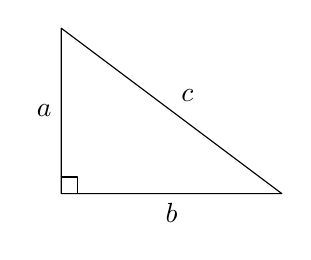
\begin{tikzpicture}[line cap=round,line join=round,>=triangle 45,x=0.7cm,y=0.7cm]
\draw (0,0)--(4,0)--(0,3)--cycle;
\draw (0.3,0)--(0.3,0.3)--(0,0.3);
\node[below] at (2,0) {$b$};
\node[left] at (0,1.5) {$a$};
\node[above right] at (2,1.5) {$c$};
\end{tikzpicture}
\end{figurehere}
\end{center}

% kuva 2: trigonometriset

\begin{center}
\begin{figurehere}
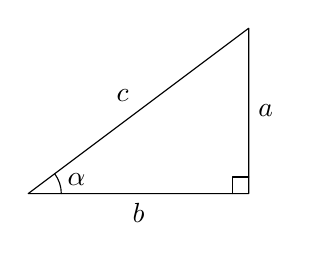
\begin{tikzpicture}[line cap=round,line join=round,>=triangle 45,x=0.7cm,y=0.7cm]
\draw (0,0)--(4,0)--(4,3)--cycle;
\draw (3.7,0)--(3.7,0.3)--(4,0.3);
\node[below] at (2,0) {$b$};
\node[right] at (4,1.5) {$a$};
\node[above left] at (2,1.5) {$c$};
\draw (0:0.6) arc (0:36.87:0.6); 
\node[right] at (26:0.6) {$\alpha$};
\end{tikzpicture}
\end{figurehere}
\end{center}

% kuva 3: suorakulmio

\begin{center}
\begin{figurehere}
\begin{tikzpicture}[line cap=round,line join=round,>=triangle 45,x=0.7cm,y=0.7cm]
\draw (0,0)--(4,0)--(4,3)--(0,3)--cycle;
\draw (0.3,0)--(0.3,0.3)--(0,0.3);
\node[below] at (2,0) {$b$};
\node[left] at (0,1.5) {$a$};
\end{tikzpicture}
\end{figurehere}
\end{center}

% kuva 4: kolmion pinta-ala

\begin{center}
\begin{figurehere}
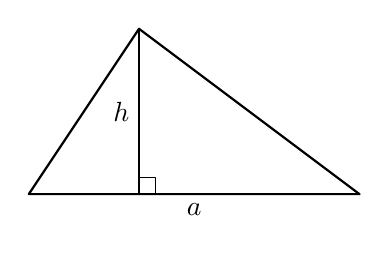
\begin{tikzpicture}[line cap=round,line join=round,>=triangle 45,x=0.7cm,y=0.7cm]
\draw[thick] (0,0)--(6,0)--(2,3)--cycle;
\draw (2,0)--(2,3);
\draw (2.3,0)--(2.3,0.3)--(2,0.3);
\node[below] at (3,0) {$a$};
\node[left] at (2,1.5) {$h$};
\end{tikzpicture}
\end{figurehere}
\end{center}

% kuva 5: kolmion pinta-ala

\begin{center}
\begin{figurehere}
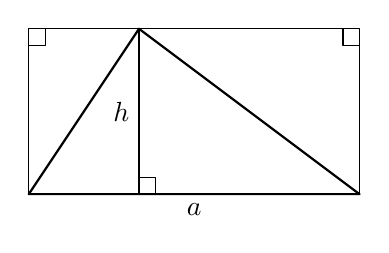
\begin{tikzpicture}[line cap=round,line join=round,>=triangle 45,x=0.7cm,y=0.7cm]
\draw[thick] (0,0)--(6,0)--(2,3)--cycle;
\draw (2,0)--(2,3);
\draw (0,0)--(0,3)--(6,3)--(6,0);
\draw (2.3,0)--(2.3,0.3)--(2,0.3);
\draw (0.3,3)--(0.3,2.7)--(0,2.7);
\draw (5.7,3)--(5.7,2.7)--(6,2.7);
\node[below] at (3,0) {$a$};
\node[left] at (2,1.5) {$h$};
\end{tikzpicture}
\end{figurehere}
\end{center}

% kuva 6: kolmion kulmien summa

\begin{center}
\begin{figurehere}
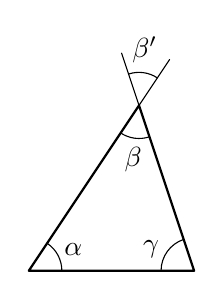
\begin{tikzpicture}[line cap=round,line join=round,>=triangle 45,x=0.7cm,y=0.7cm]
\draw[thick] (0,0)--(3,0)--(2,3)--cycle;
\draw (0:0.6) arc (0:56.31:0.6); 
\node [right] at (39:0.6) {$\alpha$};
\begin{scope}[shift={(2,3)}]
\draw (236.31:0.6) arc (236.31:288.43:0.6); 
\node [below] at (260:0.6) {$\beta$};
\draw (108.43:1)--(0,0)--(56.31:1);
\draw (56.31:0.6) arc (56.31:108.43:0.6); 
\node [above] at (80:0.6) {$\beta'$};
\end{scope}
\begin{scope}[shift={(3,0)}]
\draw (108.43:0.6) arc (108.43:180:0.6); 
\node [left] at (140:0.6) {$\gamma$};
\end{scope}
\end{tikzpicture}
\end{figurehere}
\end{center}

% kuva 7: kolmion kulmien summa

\begin{center}
\begin{figurehere}
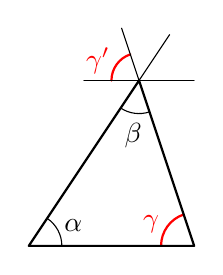
\begin{tikzpicture}[line cap=round,line join=round,>=triangle 45,x=0.7cm,y=0.7cm]
\begin{scope}[shift={(2,3)}]
\draw (236.31:0.6) arc (236.31:288.43:0.6); 
\node [below] at (260:0.6) {$\beta$};
\draw[thick, color = red] (180:0.5) arc (180:108.43:0.5); 
\node [left, color = red] at (135:0.5) {$\gamma'$};
%\draw (56.31:0.6) arc (56.31:108.43:0.6); 
%\node [above] at (80:0.6) {$\beta'$};
\draw (108.43:1)--(0,0)--(56.31:1);
\draw (-1,0)--(1,0);
\end{scope}
\begin{scope}[shift={(3,0)}]
\draw[thick, color = red]  (108.43:0.6) arc (108.43:180:0.6); 
\node [left, color = red] at (140:0.6) {$\gamma$};
\end{scope}
\draw[thick] (0,0)--(3,0)--(2,3)--cycle;
\draw (0:0.6) arc (0:56.31:0.6); 
\node [right] at (39:0.6) {$\alpha$};
\end{tikzpicture}
\end{figurehere}
\end{center}

% kuva 8: kolmion kulmien summa

\begin{center}
\begin{figurehere}
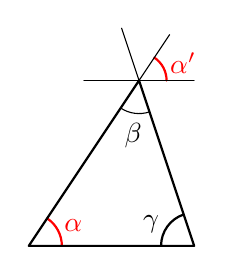
\begin{tikzpicture}[line cap=round,line join=round,>=triangle 45,x=0.7cm,y=0.7cm]
\begin{scope}[shift={(2,3)}]
\draw (236.31:0.6) arc (236.31:288.43:0.6); 
\node [below] at (260:0.6) {$\beta$};
\draw[thick, color = red] (0:0.5) arc (0:56.31:0.5); 
\node [right, color = red] at (39:0.5) {$\alpha'$};
%\draw[thick, color = red] (180:0.5) arc (180:108.43:0.5); 
%\node [left, color = red] at (135:0.5) {$\gamma'$};
%\draw (56.31:0.6) arc (56.31:108.43:0.6); 
%\node [above] at (80:0.6) {$\beta'$};
\draw (108.43:1)--(0,0)--(56.31:1);
\draw (-1,0)--(1,0);
\end{scope}
\begin{scope}[shift={(3,0)}]
\draw[thick]  (108.43:0.6) arc (108.43:180:0.6); 
\node [left] at (140:0.6) {$\gamma$};
\end{scope}
\draw [thick, color = red](0:0.6) arc (0:56.31:0.6); 
\node [right, color = red] at (39:0.6) {$\alpha$};
\draw[thick] (0,0)--(3,0)--(2,3)--cycle;
\end{tikzpicture}
\end{figurehere}
\end{center}

% kuva 9: kolmion kulmien summa

\begin{center}
\begin{figurehere}
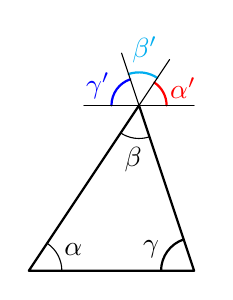
\begin{tikzpicture}[line cap=round,line join=round,>=triangle 45,x=0.7cm,y=0.7cm]
\begin{scope}[shift={(2,3)}]
\draw (236.31:0.6) arc (236.31:288.43:0.6); 
\node [below] at (260:0.6) {$\beta$};
\draw[thick, color = red] (0:0.5) arc (0:56.31:0.5); 
\node [right, color = red] at (39:0.5) {$\alpha'$};
\draw[thick, color = blue] (180:0.5) arc (180:108.43:0.5); 
\node [left, color = blue] at (135:0.5) {$\gamma'$};
\draw [thick, color = cyan] (56.31:0.6) arc (56.31:108.43:0.6); 
\node [above, color=cyan] at (80:0.6) {$\beta'$};
\draw (108.43:1)--(0,0)--(56.31:1);
\draw (-1,0)--(1,0);
\end{scope}
\begin{scope}[shift={(3,0)}]
\draw[thick]  (108.43:0.6) arc (108.43:180:0.6); 
\node [left] at (140:0.6) {$\gamma$};
\end{scope}
\draw (0:0.6) arc (0:56.31:0.6); 
\node [right] at (39:0.6) {$\alpha$};
\draw[thick] (0,0)--(3,0)--(2,3)--cycle;
\end{tikzpicture}
\end{figurehere}
\end{center}

% kuva 10: tylpän kulman kosini ja sini

\begin{center}
\begin{figurehere}
\begin{tikzpicture}[line cap=round,line join=round,>=triangle 45,x=2cm,y=2cm]
\draw[->,color=gray] (-1.5,0) -- (1.5,0);
%tiksut ja viivat
\foreach \x in {-1,1}
{%\draw[dashed, color= lightgray] (\x,-2.5)--(\x,4.5);
\draw[shift={(\x,0)},color=black] (0pt,2pt) -- (0pt,-2pt);
}
\node [below] at (1.5,0) {$x$};

%y-akseli
\draw[->,color=gray] (0,-0.5) -- (0,1.5);
%tiksut ja viivat
\foreach \y in {-1,1}
{
%\draw[dashed, color=lightgray] (-2.5,\y)--(3.5,\y);
\draw[shift={(0,\y)},color=black] (2pt,0pt) -- (-2pt,0pt);
}
\node [left] at (0,1.5) {$y$};
\draw [thick] (1,0)--(0,0)--(140:1);
\draw[fill] (140:1) circle [radius = 1.5pt];
\draw[dashed] (-0.766,0)--(140:1)--(0,0.643);
\node [right] at (0,0.643) {$\sin \alpha$};
\node [below] at (-0.65,0) {$\cos \alpha$};
\node [below] at (-1.05,-0.05) {$-1$};
\node [below] at (1,-0.05) {$1$};
\node [right] at (0,1) {$1$};
\draw (0:0.15) arc (0:140:0.15); 
\node [above right] at (75:0.1) {$\alpha$};
\node [above right] at (140:0.5) {$1$};
\node [above left] at (-0.766,0.643) {$(\cos \alpha, \sin \alpha)$};
\end{tikzpicture}
\end{figurehere}
\end{center}

% kuva 11: tylpän kulman kosini ja sini

\begin{center}
\begin{figurehere}
\begin{tikzpicture}[line cap=round,line join=round,>=triangle 45,x=2cm,y=2cm]
\draw[->,color=gray] (-1.5,0) -- (1.5,0);
%tiksut ja viivat
\foreach \x in {-1,1}
{%\draw[dashed, color= lightgray] (\x,-2.5)--(\x,4.5);
\draw[shift={(\x,0)},color=black] (0pt,2pt) -- (0pt,-2pt);
}
\node [below] at (1.5,0) {$x$};

%y-akseli
\draw[->,color=gray] (0,-0.5) -- (0,1.5);
%tiksut ja viivat
\foreach \y in {-1,1}
{
%\draw[dashed, color=lightgray] (-2.5,\y)--(3.5,\y);
\draw[shift={(0,\y)},color=black] (2pt,0pt) -- (-2pt,0pt);
}
\node [left] at (0,1.5) {$y$};
\draw [thick] (1,0)--(0,0)--(140:1);
%\draw[fill] (140:1) circle [radius = 1.5pt];
%\draw[dashed] (-0.766,0)--(140:1)--(0,0.643);
%\node [right] at (0,0.643) {$\sin \alpha$};
%\node [below] at (-0.65,0) {$\cos \alpha$};
\node [below] at (-1.05,-0.05) {$-1$};
\node [below] at (1,-0.05) {$1$};
\node [right] at (0,1) {$1$};
\draw (0:0.15) arc (0:140:0.15); 
\node [above right] at (75:0.1) {$\alpha$};
\node [above right] at (140:0.5) {$1$};
%\node [above left] at (-0.766,0.643) {$(\cos \alpha, \sin \alpha)$};
\end{tikzpicture}
\end{figurehere}
\end{center}

% kuva 12: sinilause

\begin{center}
\begin{figurehere}
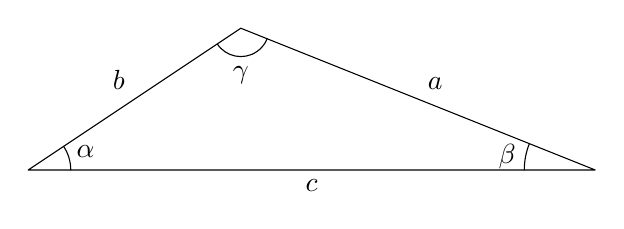
\begin{tikzpicture}[line cap=round,line join=round,>=triangle 45,x=0.9cm,y=0.9cm]
\begin{scope}[shift={(3,2)}]
\draw   (213.69:0.4) arc (213.69:338.2:0.4); 
\node [below] at (270:0.4) {$\gamma$};
\end{scope}
%
\begin{scope}[shift={(8,0)}]
\draw   (158.20:1) arc (158.20:180:1); 
\node [left] at (169:1) {$\beta$};
\end{scope}
\draw (0:0.6) arc (0:33.69:0.6); 
\node [right] at (25:0.6) {$\alpha$};
\draw (0,0)--(8,0)--(3,2)--cycle;
\node[below] at (4,0) {$c$};
\node[above right] at (5.5,1) {$a$};
\node[above left] at (1.5,1) {$b$};
\end{tikzpicture}
\end{figurehere}
\end{center}

% kuva 13: kosinilause

\begin{center}
\begin{figurehere}
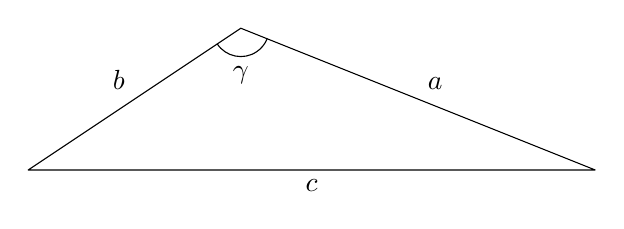
\begin{tikzpicture}[line cap=round,line join=round,>=triangle 45,x=0.9cm,y=0.9cm]
\begin{scope}[shift={(3,2)}]
\draw   (213.69:0.4) arc (213.69:338.2:0.4); 
\node [below] at (270:0.4) {$\gamma$};
\end{scope}
%
%\begin{scope}[shift={(8,0)}]
%\draw   (158.20:1) arc (158.20:180:1); 
%\node [left] at (169:1) {$\beta$};
%\end{scope}
%\draw (0:0.6) arc (0:33.69:0.6); 
%\node [right] at (25:0.6) {$\alpha$};
\draw (0,0)--(8,0)--(3,2)--cycle;
\node[below] at (4,0) {$c$};
\node[above right] at (5.5,1) {$a$};
\node[above left] at (1.5,1) {$b$};
\end{tikzpicture}
\end{figurehere}
\end{center}

% kuva 14: yhdenmuotoisuus

\begin{center}
\begin{figurehere}
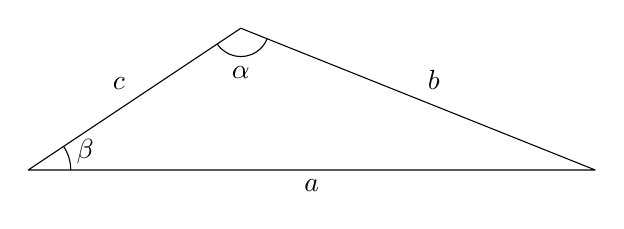
\begin{tikzpicture}[line cap=round,line join=round,>=triangle 45,x=0.9cm,y=0.9cm]
\begin{scope}[shift={(3,2)}]
\draw   (213.69:0.4) arc (213.69:338.2:0.4); 
\node [below] at (270:0.4) {$\alpha$};
\end{scope}
%
\draw (0:0.6) arc (0:33.69:0.6); 
\node [right] at (25:0.6) {$\beta$};
\draw (0,0)--(8,0)--(3,2)--cycle;
\node[below] at (4,0) {$a$};
\node[above right] at (5.5,1) {$b$};
\node[above left] at (1.5,1) {$c$};
\end{tikzpicture}
\hspace{0.5cm}
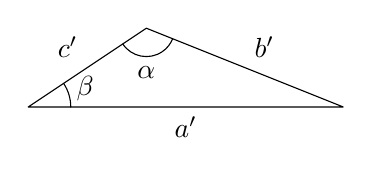
\begin{tikzpicture}[line cap=round,line join=round,>=triangle 45,x=0.5cm,y=0.5cm]
\begin{scope}[shift={(3,2)}]
\draw   (213.69:0.72) arc (213.69:338.2:0.72); 
\node [below] at (270:0.72) {$\alpha$};
\end{scope}
%
\draw (0:1.08) arc (0:33.69:1.08); 
\node [right] at (25:1.08) {$\beta$};
\draw (0,0)--(8,0)--(3,2)--cycle;
\node[below] at (4,0) {$a'$};
\node[above right] at (5.5,1) {$b'$};
\node[above left] at (1.5,1) {$c'$};
\end{tikzpicture}
\end{figurehere}
\end{center}

% kuva 15: Kolmion pinta-ala

\begin{center}
\begin{figurehere}
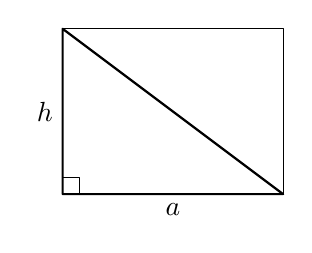
\begin{tikzpicture}[line cap=round,line join=round,>=triangle 45,x=0.7cm,y=0.7cm]
\draw (0,3)--(4,3)--(4,0);
\draw [thick] (0,0)--(4,0)--(0,3)--cycle;
\draw (0.3,0)--(0.3,0.3)--(0,0.3);
\node[below] at (2,0) {$a$};
\node[left] at (0,1.5) {$h$};
%\node[above right] at (2,1.5) {$c$};
\end{tikzpicture}
\end{figurehere}
\end{center}

% kuva 16: Kolmion pinta-ala

\begin{center}
\begin{figurehere}
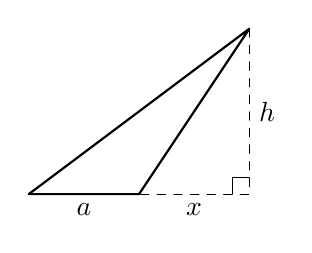
\begin{tikzpicture}[line cap=round,line join=round,>=triangle 45,x=0.7cm,y=0.7cm]
\draw [dashed] (4,3)--(4,0)--(2,0);
\draw [thick] (0,0)--(2,0)--(4,3)--cycle;
\draw (3.7,0)--(3.7,0.3)--(4,0.3);
\node[below] at (1,0) {$a$};
\node[below] at (3,0) {$x$};
\node[right] at (4,1.5) {$h$};
%\node[above right] at (2,1.5) {$c$};
\end{tikzpicture}
\end{figurehere}
\end{center}

% kuva 17: Suora kulma

\begin{center}
\begin{figurehere}
\begin{tikzpicture}[line cap=round,line join=round,>=triangle 45,x=0.7cm,y=0.7cm]
\draw [thick] (0,2)--(0,0)--(2,0);
\draw (0.3,0)--(0.3,0.3)--(0,0.3);
\end{tikzpicture}
\end{figurehere}
\end{center}

% kuva 18: Oikokulma
\vspace{1cm}

\begin{center}
\begin{figurehere}
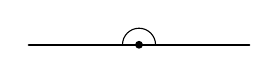
\begin{tikzpicture}[line cap=round,line join=round,>=triangle 45,x=0.7cm,y=0.7cm]
\draw [thick] (-2,0)--(0,0)--(2,0);
\draw (0:0.3) arc (0:180:0.3);
\draw [fill] (0,0) circle [radius = 1.2pt];
\end{tikzpicture}
\end{figurehere}
\end{center}

% kuva 19: Vieruskulma
\vspace{1cm}

\begin{center}
\begin{figurehere}
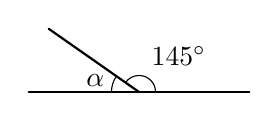
\begin{tikzpicture}[line cap=round,line join=round,>=triangle 45,x=0.7cm,y=0.7cm]
\draw [thick] (-2,0)--(0,0)--(2,0);
\draw [thick] (0,0)--(145:2);
\draw (0:0.3) arc (0:145:0.3);
\draw (145:0.5) arc (145:180:0.5);
\node [above right] at (80:0.3) {$145^\circ$};
\node [left] at (155:0.5) {$\alpha$};
%\draw [fill] (0,0) circle [radius = 1.2pt];
\end{tikzpicture}
\end{figurehere}
\end{center}

% kuva 19: Vieruskulma
\vspace{1cm}

\begin{center}
\begin{figurehere}
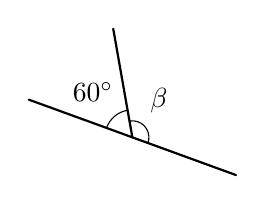
\begin{tikzpicture}[line cap=round,line join=round,>=triangle 45,x=0.7cm,y=0.7cm]
\draw [thick] (160:2)--(-20:2);
\draw [thick] (100:2)--(0:0);
\draw (100:0.5) arc (100:160:0.5);
\draw (-20:0.3) arc (-20:100:0.3);
\node [above right] at (60:0.3) {$\beta$};
\node [above left] at (110:0.5) {$60^\circ$};
%\draw [fill] (0,0) circle [radius = 1.2pt];
\end{tikzpicture}
\end{figurehere}
\end{center}

% kuva 20: Vieruskulma
\vspace{1cm}

\begin{center}
\begin{figurehere}
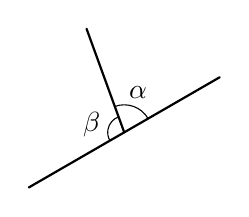
\begin{tikzpicture}[line cap=round,line join=round,>=triangle 45,x=0.7cm,y=0.7cm]
\draw [thick] (30:2)--(210:2);
\draw [thick] (110:2)--(0:0);
\draw (30:0.5) arc (30:110:0.5);
\draw (110:0.3) arc (110:210:0.3);
\node [above] at (60:0.5) {$\alpha$};
\node [left] at (150:0.3) {$\beta$};
%\draw [fill] (0,0) circle [radius = 1.2pt];
\end{tikzpicture}
\end{figurehere}
\end{center}

% kuva 21: Ristikulma
\vspace{1cm}

\begin{center}
\begin{figurehere}
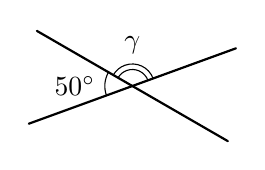
\begin{tikzpicture}[line cap=round,line join=round,>=triangle 45,x=0.7cm,y=0.7cm]
\draw [thick] (150:2)--(330:2);
\draw [thick] (20:2)--(200:2);
\draw (20:0.4) arc (20:150:0.4);
\draw (20:0.3) arc (20:150:0.3);
\draw (150:0.5) arc (150:200:0.5);
\node [above] at (90:0.4) {$\gamma$};
\node [left] at (180:0.5) {$50^\circ$};
%\draw [fill] (0,0) circle [radius = 1.2pt];
\end{tikzpicture}
\end{figurehere}
\end{center}

% kuva 21: Ristikulma
\vspace{1cm}

\begin{center}
\begin{figurehere}
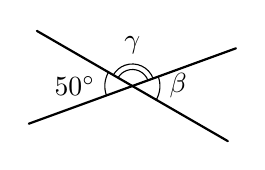
\begin{tikzpicture}[line cap=round,line join=round,>=triangle 45,x=0.7cm,y=0.7cm]
\draw [thick] (150:2)--(330:2);
\draw [thick] (20:2)--(200:2);
\draw (20:0.4) arc (20:150:0.4);
\draw (20:0.3) arc (20:150:0.3);
\draw (150:0.5) arc (150:200:0.5);
\draw (-30:0.5) arc (-30:20:0.5);
\node [above] at (90:0.4) {$\gamma$};
\node [left] at (180:0.5) {$50^\circ$};
\node [right] at (0:0.5) {$\beta$};
%\draw [fill] (0,0) circle [radius = 1.2pt];
\end{tikzpicture}
\end{figurehere}
\end{center}

% kuva 22: Ristikulma
\vspace{1cm}

\begin{center}
\begin{figurehere}
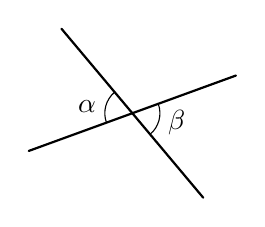
\begin{tikzpicture}[line cap=round,line join=round,>=triangle 45,x=0.7cm,y=0.7cm]
\draw [thick] (130:2)--(310:2);
\draw [thick] (20:2)--(200:2);
%\draw (20:0.4) arc (20:150:0.4);
\draw (-50:0.5) arc (-50:20:0.5);
\draw (130:0.5) arc (130:200:0.5);
%\node [above] at (90:0.4) {$\gamma$};
\node [left] at (165:0.5) {$\alpha$};
\node [right] at (-20:0.5) {$\beta$};
%\draw [fill] (0,0) circle [radius = 1.2pt];
\end{tikzpicture}
\end{figurehere}
\end{center}

% kuva 23: Kolmion pinta-ala tehtävään

\begin{center}
\begin{figurehere}
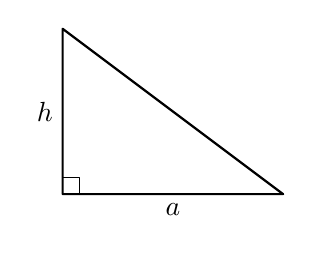
\begin{tikzpicture}[line cap=round,line join=round,>=triangle 45,x=0.7cm,y=0.7cm]
%\draw (0,3)--(4,3)--(4,0);
\draw [thick] (0,0)--(4,0)--(0,3)--cycle;
\draw (0.3,0)--(0.3,0.3)--(0,0.3);
\node[below] at (2,0) {$a$};
\node[left] at (0,1.5) {$h$};
%\node[above right] at (2,1.5) {$c$};
\end{tikzpicture}
\end{figurehere}
\end{center}

% kuva 24: Samankohtaiset kulmat

\begin{center}
\begin{figurehere}
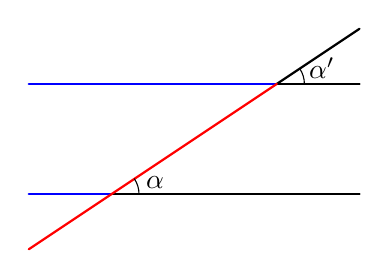
\begin{tikzpicture}[line cap=round,line join=round,>=triangle 45,x=0.7cm,y=0.7cm]
\draw [thick] (4,0)--(-0.5,0);
\draw [thick, color = blue] (-0.5,0)--(-2,0);
\draw [thick] (4,2)--(2.5,2);
\draw [thick, color = blue] (2.5,2)--(-2,2);
\draw [thick] (2.5,2)--(4,3);
\draw [thick, color = red] (2.5,2)--(-2,-1);
\begin{scope}[shift={(-0.5,0)}]
\draw (0:0.5) arc (0:33.69:0.5);
\node[right] at (25:0.5) {$\alpha$};
\end{scope}
\begin{scope}[shift={(2.5,2)}]
\draw (0:0.5) arc (0:33.69:0.5);
\node[right] at (35:0.5) {$\alpha'$};
\end{scope}
\end{tikzpicture}
\end{figurehere}
\end{center}

% kuva 25: Samankohtaiset kulmat

\begin{center}
\begin{figurehere}
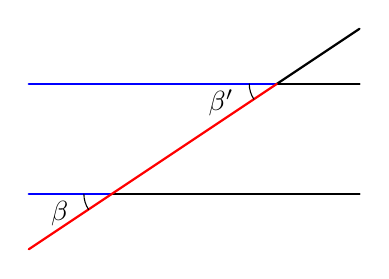
\begin{tikzpicture}[line cap=round,line join=round,>=triangle 45,x=0.7cm,y=0.7cm]
\draw [thick] (4,0)--(-0.5,0);
\draw [thick, color = blue] (-0.5,0)--(-2,0);
\draw [thick] (4,2)--(2.5,2);
\draw [thick, color = blue] (2.5,2)--(-2,2);
\draw [thick] (2.5,2)--(4,3);
\draw [thick, color = red] (2.5,2)--(-2,-1);
\begin{scope}[shift={(-0.5,0)}]
\draw (180:0.5) arc (180:213.69:0.5);
\node[left] at (210:0.7) {$\beta$};
\end{scope}
\begin{scope}[shift={(2.5,2)}]
\draw (180:0.5) arc (180:213.69:0.5);
\node[left] at (210:0.7) {$\beta'$};
\end{scope}
\end{tikzpicture}
\end{figurehere}
\end{center}

% kuva 26: Samankohtaiset kulmat

\begin{center}
\begin{figurehere}
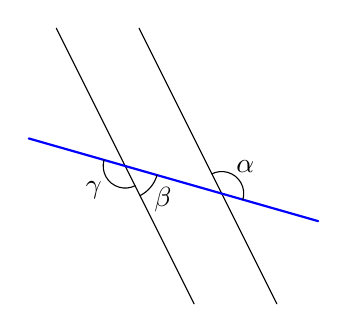
\begin{tikzpicture}[line cap=round,line join=round,>=triangle 45,x=0.7cm,y=0.7cm]
\draw (0.5,4)--(3,-1);
\draw (2,4)--(4.5,-1);
\draw [thick, color = blue, domain=0:5.25] plot (\x, {(-1/3.5)*\x+2});
\begin{scope}[shift={(7/4,1.5)}]
\draw (164.05:0.4) arc (164.05:296.57:0.4);
\node[left] at (240:0.5) {$\gamma$};
\draw (296.57:0.6) arc (296.57:344.05:0.6);
\node[right] at (300:0.7) {$\beta$};
\end{scope}
\begin{scope}[shift={(3.5,1)}]
\draw (-15.95:0.4) arc (-15.95:116.57:0.4);
\node[right] at (80:0.5) {$\alpha$};
\end{scope}
\end{tikzpicture}
\end{figurehere}
\end{center}

% kuva 27: Yhdenmuotoiset kolmiot

\begin{center}
\begin{figurehere}
\begin{tikzpicture}[line cap=round,line join=round,>=triangle 45,x=0.7cm,y=0.7cm]
\draw (0,0)--(4,0)--(3,2)--cycle;
\draw (0:0.4) arc (0:33.69:0.4);
\draw (0:0.5) arc (0:33.69:0.5);
\node [left] at (0,0) {$A$};
\node [right] at (4,0) {$B$};
\node [above] at (3,2) {$C$};
\begin{scope}[shift={(3,2)}]
\draw (213.69:0.4) arc (213.69:296.57:0.4);
\end{scope}
%
%\begin{scope}[shift={(6,0)}, scale = 0.5]
%\draw (0,0)--(4,0)--(3,2)--cycle;
%\draw (0:0.4) arc (0:33.69:0.4);
%\draw (0:0.5) arc (0:33.69:0.5);
%\node [left] at (0,0) {$D$};
%\node [right] at (4,0) {$E$};
%\node [above] at (3,2) {$F$};
%\begin{scope}[shift={(3,2)}]
%\draw (213.69:0.4) arc (213.69:296.57:0.4);
%\end{scope}
%\end{scope}
%\begin{scope}[shift={(0,2)}, rotate = 60]
%\draw (0,0)--(4,0)--(3,2)--cycle;
%\node [below] at (0,0) {$G$};
%\node [right] at (4,0) {$H$};
%\node [left] at (3,2) {$I$};
%\draw (0:0.4) arc (0:33.69:0.4);
%\draw (0:0.5) arc (0:33.69:0.5);
%\begin{scope}[shift={(3,2)}]
%\draw (213.69:0.4) arc (213.69:296.57:0.4);
%\end{scope}
%\end{scope}
\begin{scope}[shift={(8,3.5)}, rotate = 180, scale = 0.75]
\draw (0,0)--(4,0)--(3,2)--cycle;
\node [right] at (0,0) {$J$};
\node [left] at (4,0) {$K$};
\node [below] at (3,2) {$L$};
\draw (0:0.4) arc (0:33.69:0.4);
\draw (0:0.5) arc (0:33.69:0.5);
\begin{scope}[shift={(3,2)}]
\draw (213.69:0.4) arc (213.69:296.57:0.4);
\end{scope}
\end{scope}
\end{tikzpicture}
\end{figurehere}
\end{center}


% kuva 28: yhdenmuotoisuus tehtävään

\begin{center}
\begin{figurehere}
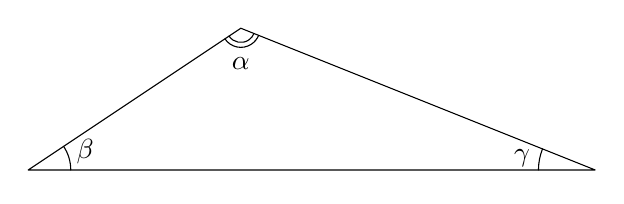
\begin{tikzpicture}[line cap=round,line join=round,>=triangle 45,x=0.9cm,y=0.9cm]
\begin{scope}[shift={(3,2)}]
\draw   (213.69:0.2) arc (213.69:338.2:0.2); 
\draw   (213.69:0.27) arc (213.69:338.2:0.27); 
\node [below] at (270:0.28) {$\alpha$};
\end{scope}
%
\begin{scope}[shift={(8,0)}]
\draw   (158.2:0.8) arc (158.2:180:0.8); 
%\draw   (213.69:0.27) arc (213.69:338.2:0.27); 
\node [left] at (168:0.8) {$\gamma$};
\end{scope}
%
\draw (0:0.6) arc (0:33.69:0.6); 
\node [right] at (25:0.6) {$\beta$};
\draw (0,0)--(8,0)--(3,2)--cycle;
%\node[below] at (4,0) {$a$};
%\node[above right] at (5.5,1) {$b$};
%\node[above left] at (1.5,1) {$c$};
\end{tikzpicture}
\hspace{0.5cm}
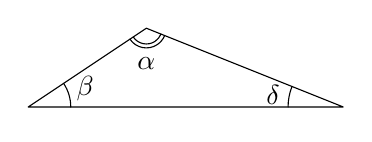
\begin{tikzpicture}[line cap=round,line join=round,>=triangle 45,x=0.5cm,y=0.5cm]
\begin{scope}[shift={(3,2)}]
\draw   (213.69:0.4) arc (213.69:338.2:0.4); 
\draw   (213.69:0.5) arc (213.69:338.2:0.5); 
\node [below] at (270:0.5) {$\alpha$};
\end{scope}
%
\begin{scope}[shift={(8,0)}]
\draw   (158.2:1.4) arc (158.2:180:1.4); 
%\draw   (213.69:0.27) arc (213.69:338.2:0.27); 
\node [left] at (167:1.4) {$\delta$};
\end{scope}
%
\draw (0:1.08) arc (0:33.69:1.08); 
\node [right] at (25:1.08) {$\beta$};
\draw (0,0)--(8,0)--(3,2)--cycle;
%\node[below] at (4,0) {$a'$};
%\node[above right] at (5.5,1) {$b'$};
%\node[above left] at (1.5,1) {$c'$};
\end{tikzpicture}
\end{figurehere}
\end{center}

% kuva 29: yhdenmuotoisuus tehtävään

\begin{center}
\begin{figurehere}
\begin{tikzpicture}[line cap=round,line join=round,>=triangle 45,x=0.9cm,y=0.9cm]
\draw (-2.4,0)--(4,0);
\draw (221.65:3)--(0,0) node [midway, below right] {$3$};
\draw (0,0)--(41.65:5) node [midway, above left] {$5$};
\draw [thick, color = blue] (221.65:3)--(-2.4,0) node [midway, left] {$2$};
\draw [thick, color = blue] (41.65:5)--(4,0);
\node[below right] at (4,0) {$C$};
\node[above right] at (41.65:5) {$D$};
\node[above left] at (-2.4,0) {$A$};
\node[below left] at (221.65:3) {$B$};
\node[below] at (2,0) {$4$};
\node[above] at (0,0) {$O$};
\draw [fill] (0,0) circle [radius = 1pt];
\end{tikzpicture}
\end{figurehere}
\end{center}

% kuva 30: Pythagoraan lauseen perustelu 1

\begin{center}
\begin{figurehere}
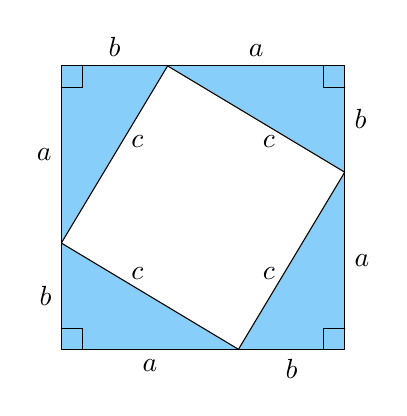
\begin{tikzpicture}[line cap=round,line join=round,>=triangle 45,x=0.9cm,y=0.9cm]
\draw [fill, color = LightSkyBlue] (0,0)--(4,0)--(4,4)--(0,4)--cycle;
\draw [fill, color = white] (2.5,0)--(4,2.5)--(1.5,4)--(0,1.5)--cycle;
\draw (0,0)--(4,0)--(4,4)--(0,4)--cycle;
\draw (2.5,0)--(4,2.5)--(1.5,4)--(0,1.5)--cycle;
\draw (0.3,0)--(0.3,0.3)--(0,0.3);
\draw (3.7,0)--(3.7,0.3)--(4,0.3);
\draw (3.7,4)--(3.7,3.7)--(4,3.7);
\draw (0.3,4)--(0.3,3.7)--(0,3.7);
\node[right] at (4,3.25) {$b$};
\node[right] at (4,1.25) {$a$};
\node[left] at (0,2.75) {$a$};
\node[left] at (0,0.75) {$b$};
\node[below] at (1.25,0) {$a$};
\node[below] at (3.25,0) {$b$};
\node[above] at (2.75,4) {$a$};
\node[above] at (0.75,4) {$b$};
\node[above right] at (0.85,0.85) {$c$};
\node[above left] at (3.15,0.85) {$c$};
\node[below right] at (0.85,3.15) {$c$};
\node[below left] at (3.15,3.15) {$c$};
\end{tikzpicture}
\end{figurehere}
\end{center}

% kuva 31: Pythagoraan lauseen perustelu 2

\begin{center}
\begin{figurehere}
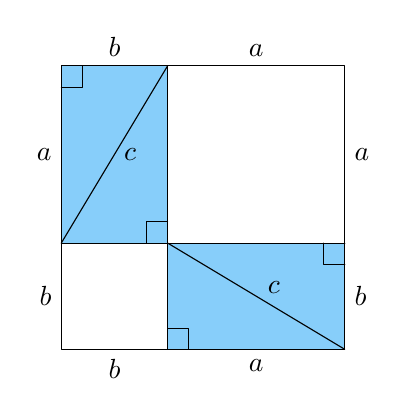
\begin{tikzpicture}[line cap=round,line join=round,>=triangle 45,x=0.9cm,y=0.9cm]
\draw [fill, color = LightSkyBlue] (0,4)--(0,1.5)--(1.5,1.5)--(1.5,4)--cycle;
\draw [fill, color = LightSkyBlue] (1.5,0)--(4,0)--(4,1.5)--(1.5,1.5)--cycle;
\draw (0,0)--(4,0)--(4,4)--(0,4)--cycle;
\draw (1.5,0)--(1.5,4);
\draw (0,1.5)--(4,1.5);
\draw (0,1.5)--(1.5,4);
\draw (1.5,1.5)--(4,0);
\draw (1.8,0)--(1.8,0.3)--(1.5,0.3);
\draw (3.7,1.5)--(3.7,1.2)--(4,1.2);
\draw (1.2,1.5)--(1.2,1.8)--(1.5,1.8);
\draw (0,3.7)--(0.3,3.7)--(0.3,4);
\node[right] at (4,2.75) {$a$};
\node[right] at (4,0.75) {$b$};
\node[left] at (0,2.75) {$a$};
\node[left] at (0,0.75) {$b$};
\node[below] at (0.75,0) {$b$};
\node[below] at (2.75,0) {$a$};
\node[above] at (2.75,4) {$a$};
\node[above] at (0.75,4) {$b$};
%\node[above right] at (0.85,0.85) {$c$};
\node[below] at (3,1.1) {$c$};
\node[right] at (0.75,2.75) {$c$};
%\node[below left] at (3.15,3.15) {$c$};
\end{tikzpicture}
\end{figurehere}
\end{center}

% kuva 32: Pythagoraan lauseen perustelu 3

\begin{center}
\begin{figurehere}
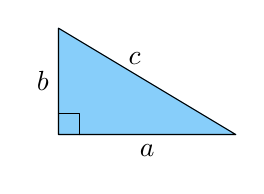
\begin{tikzpicture}[line cap=round,line join=round,>=triangle 45,x=0.9cm,y=0.9cm]
\draw [fill, color = LightSkyBlue] (0,0)--(2.5,0)--(0,1.5)--cycle;
\draw (0,0)--(2.5,0)--(0,1.5)--cycle;
\draw (0.3,0)--(0.3,0.3)--(0,0.3);
\node[left] at (0,0.75) {$b$};
\node[below] at (1.25,0) {$a$};
\node[above right] at (0.85,0.85) {$c$};
\end{tikzpicture}
\end{figurehere}
\end{center}

% kuva 33: Suorakulmainen kolmio

\begin{center}
\begin{figurehere}
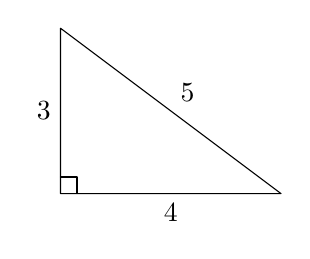
\begin{tikzpicture}[line cap=round,line join=round,>=triangle 45,x=0.7cm,y=0.7cm]
\draw (0,0)--(4,0)--(0,3)--cycle;
\draw (0.3,0)--(0.3,0.3)--(0,0.3);
\node[left] at (0,1.5) {$3$};
\node[below] at (2,0) {$4$};
\node[above right] at (2,1.5) {$5$};
\end{tikzpicture}
\end{figurehere}
\end{center}

% kuva 33: Suorakulmainen kolmio

\begin{center}
\begin{figurehere}
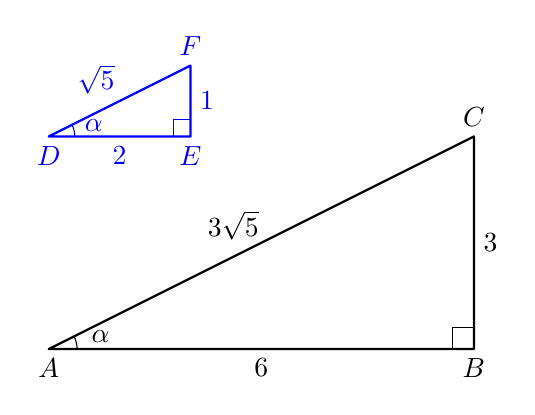
\begin{tikzpicture}[line cap=round,line join=round,>=triangle 45,x=0.9cm,y=0.9cm]
\draw [thick] (0,0)--(6,0)--(6,3)--cycle;
\draw (5.7,0)--(5.7,0.3)--(6,0.3);
\draw  (0:0.4) arc (0:26.57:0.4); 
\node [right] at (21:0.5) {$\alpha$};
\node[right] at (6,1.5) {$3$};
\node[below] at (3,0) {$6$};
\node[below] at (0,0) {$A$};
\node[below] at (6,0) {$B$};
\node[above] at (6,3) {$C$};
\node[above left] at (3.1,1.4) {$3\sqrt{5}$};
\begin{scope}[shift={(0,3)}, scale = (1/3)]
\draw[thick, color = blue] (0,0)--(6,0)--(6,3)--cycle;
\draw[color = blue] (5.3,0)--(5.3,0.7)--(6,0.7);
\draw[color = blue]  (0:1.1) arc (0:26.57:1.1); 
\node [right, color = blue] at (22:1.2) {$\alpha$};
\node[right, color = blue] at (6,1.5) {$1$};
\node[below, color = blue] at (3,0) {$2$};
\node[above left, color = blue] at (3.2,1.4) {$\sqrt{5}$};
\node[below, color = blue] at (0,0) {$D$};
\node[below, color = blue] at (6,0) {$E$};
\node[above, color = blue] at (6,3) {$F$};
\end{scope}
\end{tikzpicture}
\end{figurehere}
\end{center}

% kuva 34: Yhdenmuotoiset kolmiot esimerkki

\begin{center}
\begin{figurehere}
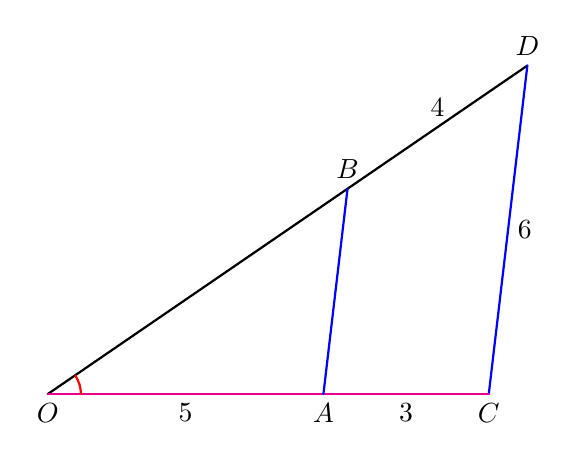
\begin{tikzpicture}[line cap=round,line join=round,>=triangle 45,x=0.7cm,y=0.7cm]
\draw [thick] (83.3:6)--(-8,0);
\draw[thick, color = blue] (0,0)--(83.3:6);
\draw[thick, color = magenta] (-8,0)--(0,0);
%\draw (3.7,0)--(3.7,0.3)--(4,0.3);
%\draw  (0:0.4) arc (0:26.57:0.4); 
%\node [right] at (21:0.5) {$\alpha$};
\node[right] at (83.3:3) {$6$};
\node[below] at (-8,0) {$O$};
\node[below] at (-3,0) {$A$};
\node[below] at (0,0) {$C$};
\node[below] at (-1.5,0) {$3$};
\node[below] at (-5.5,0) {$5$};
\node[above] at (83.3:6) {$D$};
\begin{scope}[shift={(-3,0)}]
\draw[thick, color = blue] (0,0)--(83.3:3.75);
\node[above] at (83.3:3.75) {$B$};
\end{scope}
\begin{scope}[shift={(-1.5,0)}]
\node[above] at (83.3:4.9) {$4$};
\end{scope}
\begin{scope}[shift={(-8,0)}]
\draw [thick, color = red] (0:0.6) arc (0:33.83:0.6); 
\end{scope}
\end{tikzpicture}
\end{figurehere}
\end{center}

% kuva 35: Yhdenmuotoiset kolmiot esimerkki

\begin{center}
\begin{figurehere}
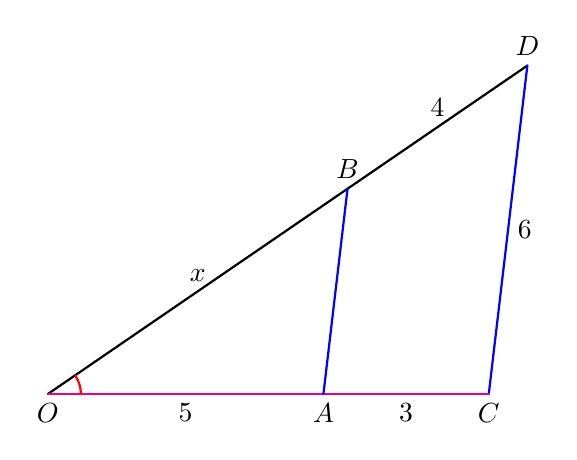
\begin{tikzpicture}[line cap=round,line join=round,>=triangle 45,x=0.7cm,y=0.7cm]
\draw [thick] (83.3:6)--(-8,0);
\draw[thick, color = blue] (0,0)--(83.3:6);
\draw[thick, color = magenta] (-8,0)--(0,0);
%\draw (3.7,0)--(3.7,0.3)--(4,0.3);
%\draw  (0:0.4) arc (0:26.57:0.4); 
%\node [right] at (21:0.5) {$\alpha$};
\node[right] at (83.3:3) {$6$};
\node[below] at (-8,0) {$O$};
\node[below] at (-3,0) {$A$};
\node[below] at (0,0) {$C$};
\node[below] at (-1.5,0) {$3$};
\node[below] at (-5.5,0) {$5$};
\node[above] at (83.3:6) {$D$};
\begin{scope}[shift={(-3,0)}]
\draw[thick, color = blue] (0,0)--(83.3:3.75);
\node[above] at (83.3:3.75) {$B$};
\end{scope}
\begin{scope}[shift={(-1.5,0)}]
\node[above] at (83.3:4.9) {$4$};
\end{scope}
\begin{scope}[shift={(-5.5,0)}]
\node[above] at (83.3:1.88) {$x$};
\end{scope}
\begin{scope}[shift={(-8,0)}]
\draw [thick, color = red] (0:0.6) arc (0:33.83:0.6); 
\end{scope}
\end{tikzpicture}
\end{figurehere}
\end{center}

% kuva 36: Trigonometriset suhteet

\begin{center}
\begin{figurehere}
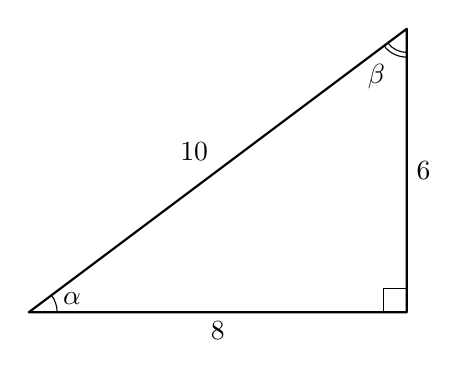
\begin{tikzpicture}[line cap=round,line join=round,>=triangle 45,x=0.6cm,y=0.6cm]
\draw [thick] (0,0)--(8,0)--(8,6)--cycle;
\draw (7.5,0)--(7.5,0.5)--(8,0.5);
\draw  (0:0.6) arc (0:36.87:0.6); 
\node [right] at (30:0.6) {$\alpha$};
\node[right] at (8,3) {$6$};
\node[below] at (4,0) {$8$};
\node[above left] at (4,3) {$10$};
\begin{scope}[shift={(8,6)}]
\draw  (216.87:0.5) arc (216.87:270:0.5); 
\draw  (216.87:0.6) arc (216.87:270:0.6); 
\node [below left] at (245:0.6) {$\beta$};
\end{scope}
\end{tikzpicture}
\end{figurehere}
\end{center}

% kuva 37: Muistikolmio

\begin{center}
\begin{figurehere}
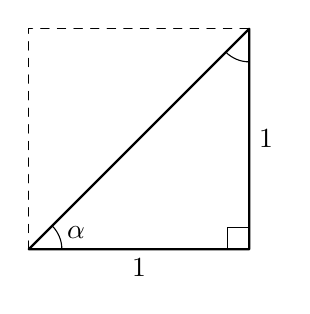
\begin{tikzpicture}[line cap=round,line join=round,>=triangle 45,x=0.7cm,y=0.7cm]
\draw [thick] (0,0)--(4,0)--(4,4)--cycle;
\draw [dashed] (0,0)--(0,4)--(4,4);
\draw (3.6,0)--(3.6,0.4)--(4,0.4);
\draw  (0:0.6) arc (0:45:0.6); 
\node [right] at (30:0.6) {$\alpha$};
\node[right] at (4,2) {$1$};
\node[below] at (2,0) {$1$};
%\node[above left] at (4,3) {$10$};
\begin{scope}[shift={(4,4)}]
\draw  (225:0.6) arc (225:270:0.6); 
%\draw  (216.87:0.6) arc (216.87:270:0.6); 
%\node [below left] at (245:0.6) {$\beta$};
\end{scope}
\end{tikzpicture}
\end{figurehere}
\end{center}

% kuva 38: Suorakulmainen kolmio tehtävään

\begin{center}
\begin{figurehere}
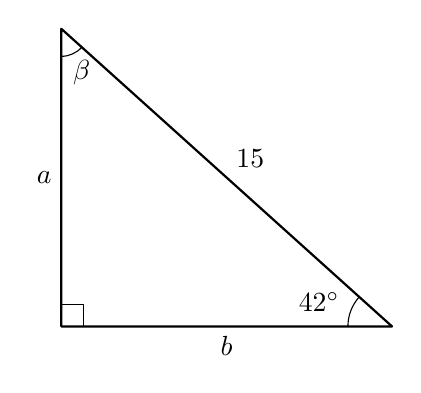
\begin{tikzpicture}[line cap=round,line join=round,>=triangle 45,x=0.7cm,y=0.7cm]
\draw [thick] (0,0)--(6,0)--(0,5.4)--cycle;
\draw (0.4,0)--(0.4,0.4)--(0,0.4);
\node[left] at (0,2.7) {$a$};
\node[below] at (3,0) {$b$};
\node[above right] at (3,2.7) {$15$};
\begin{scope}[shift={(0,5.4)}]
\draw  (-90:0.5) arc (-90:-42:0.5); 
\node [below right] at (-85:0.4) {$\beta$};
\end{scope}
\begin{scope}[shift={(6,0)}]
\draw  (138:0.8) arc (138:180:0.8); 
\node [left] at (150:0.9) {$42^\circ$};
\end{scope}
\end{tikzpicture}
\end{figurehere}
\end{center}

% kuva 39: terävän kulman kosini ja sini uudessa määritelmässä

\begin{center}
\begin{figurehere}
\begin{tikzpicture}[line cap=round,line join=round,>=triangle 45,x=2.5cm,y=2.5cm]
\draw[->,color=gray] (-1.5,0) -- (1.5,0);
%tiksut ja viivat
\foreach \x in {-1,1}
{%\draw[dashed, color= lightgray] (\x,-2.5)--(\x,4.5);
\draw[shift={(\x,0)},color=black] (0pt,2pt) -- (0pt,-2pt);
}
\node [below] at (1.5,0) {$x$};

%y-akseli
\draw[->,color=gray] (0,-0.5) -- (0,1.5);
%tiksut ja viivat
\foreach \y in {-1,1}
{
%\draw[dashed, color=lightgray] (-2.5,\y)--(3.5,\y);
\draw[shift={(0,\y)},color=black] (2pt,0pt) -- (-2pt,0pt);
}
\node [left] at (0,1.5) {$y$};
\draw [thick] (0.574,0)--(0,0)--(55:1)--cycle;
\draw (0.5,0)--(0.5,0.074)--(0.574,0.074);
%\draw[fill] (55:1) circle [radius = 1.5pt];
\draw[dashed] (0,0.819)--(55:1);
\node [right] at (0.574,0.41) {$b$};
\node [below] at (0.287,0) {$a$};
\node [above] at (55:1) {$A$};
\node [below] at (-1.05,-0.05) {$-1$};
\node [below] at (1,-0.05) {$1$};
\node [right] at (0,1) {$1$};
\draw (0:0.15) arc (0:55:0.15); 
\node [right] at (40:0.15) {$\alpha$};
\node [above left] at (55:0.5) {$1$};
%\node [above left] at (-0.766,0.643) {$(\cos \alpha, \sin \alpha)$};
\end{tikzpicture}
\end{figurehere}
\end{center}

% kuva 40: Yksikköympyrä

\begin{center}
\begin{figurehere}
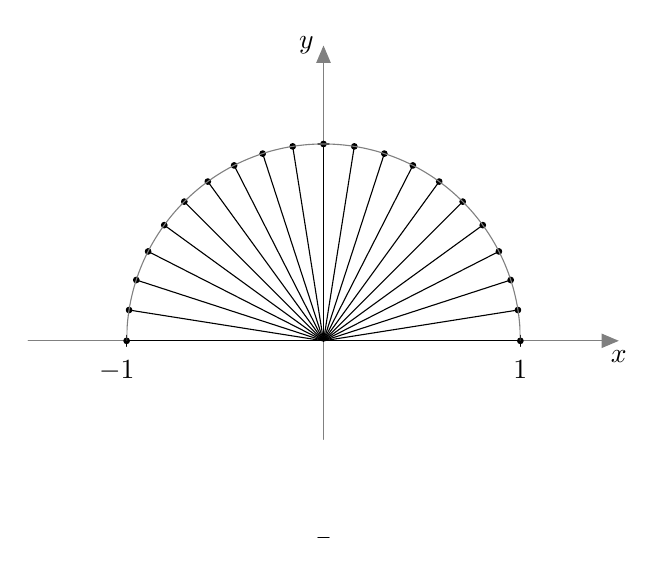
\begin{tikzpicture}[line cap=round,line join=round,>=triangle 45,x=2.5cm,y=2.5cm]
\draw[->,color=gray] (-1.5,0) -- (1.5,0);
%tiksut ja viivat
\foreach \x in {-1,1}
{
\draw[shift={(\x,0)},color=black] (0pt,2pt) -- (0pt,-2pt);
}
\node [below] at (1.5,0) {$x$};

%y-akseli
\draw[->,color=gray] (0,-0.5) -- (0,1.5);
%tiksut ja viivat
\foreach \y in {-1,1}
{
\draw[shift={(0,\y)},color=black] (2pt,0pt) -- (-2pt,0pt);
}
\node [left] at (0,1.5) {$y$};
\foreach \k in {0,...,20}
{
\draw (0,0) -- (\k*9:1);
\draw [fill] (\k*9:1) circle [radius = 1pt];
}
\begin{scope}
\clip (-1,0)--(1,0)--(1,1)--(-1,1)--cycle;
\draw[color = gray] (0,0) circle [radius = 1];
\end{scope}
\node [below] at (-1.05,-0.05) {$-1$};
\node [below] at (1,-0.05) {$1$};
\end{tikzpicture}
\end{figurehere}
\end{center}

% kuva 41: Kosinin symmetriat 1

\begin{center}
\begin{figurehere}
\begin{tikzpicture}[line cap=round,line join=round,>=triangle 45,x=2.5cm,y=2.5cm]
\draw[->,color=gray] (-1.5,0) -- (1.5,0);
%tiksut ja viivat
\foreach \x in {-1,1}
{%\draw[dashed, color= lightgray] (\x,-2.5)--(\x,4.5);
\draw[shift={(\x,0)},color=black] (0pt,2pt) -- (0pt,-2pt);
}
\node [below] at (1.5,0) {$x$};

%y-akseli
\draw[->,color=gray] (0,-0.5) -- (0,1.5);
%tiksut ja viivat
\foreach \y in {-1,1}
{
%\draw[dashed, color=lightgray] (-2.5,\y)--(3.5,\y);
\draw[shift={(0,\y)},color=black] (2pt,0pt) -- (-2pt,0pt);
}
\node [left] at (0,1.5) {$y$};
\begin{scope}
\clip (-1,0)--(1,0)--(1,1)--(-1,1)--cycle;
\draw[color = gray] (0,0) circle [radius = 1];
\end{scope}
\draw [thick, color = red] (1,0)--(0,0)--(55:1);
\draw (0.574,2pt) -- (0.574,-2pt);
\draw (2pt,0.819) -- (-2pt,0.819);
%\draw (0.5,0)--(0.5,0.074)--(0.574,0.074);
\draw[fill] (55:1) circle [radius = 1.5pt];
\draw[dashed] (0,0.819)--(55:1)--(0.574,0);
\node [left] at (0,0.819) {$b$};
\node [below] at (0.574,0) {$a$};
%\node [above] at (55:1) {$A$};
\node [below] at (-1.05,-0.05) {$-1$};
\node [below] at (1,-0.05) {$1$};
%\node [right] at (0,1) {$1$};
\draw [color = red] (0:0.15) arc (0:55:0.15); 
\node [right, color = red] at (40:0.15) {$\alpha$};
%\node [above left] at (55:0.5) {$1$};
\node [below] at (-1.05,-0.05) {$-1$};
\node [below] at (1,-0.05) {$1$};
\end{tikzpicture}
\end{figurehere}
\end{center}

% kuva 42: Kosinin symmetriat 2

\begin{center}
\begin{figurehere}
\begin{tikzpicture}[line cap=round,line join=round,>=triangle 45,x=2.5cm,y=2.5cm]
\draw[->,color=gray] (-1.5,0) -- (1.5,0);
%tiksut ja viivat
\foreach \x in {-1,1}
{%\draw[dashed, color= lightgray] (\x,-2.5)--(\x,4.5);
\draw[shift={(\x,0)},color=black] (0pt,2pt) -- (0pt,-2pt);
}
\node [below] at (1.5,0) {$x$};

%y-akseli
\draw[->,color=gray] (0,-0.5) -- (0,1.5);
%tiksut ja viivat
\foreach \y in {-1,1}
{
%\draw[dashed, color=lightgray] (-2.5,\y)--(3.5,\y);
\draw[shift={(0,\y)},color=black] (2pt,0pt) -- (-2pt,0pt);
}
\node [left] at (0,1.5) {$y$};
\begin{scope}
\clip (-1,0)--(1,0)--(1,1)--(-1,1)--cycle;
\draw[color = gray] (0,0) circle [radius = 1];
\end{scope}
\draw [thick, color = blue] (1,0)--(0,0)--(125:1);
\draw (-0.574,2pt) -- (-0.574,-2pt);
\draw (2pt,0.819) -- (-2pt,0.819);
%\draw (0.5,0)--(0.5,0.074)--(0.574,0.074);
\draw[fill] (125:1) circle [radius = 1.5pt];
\draw[dashed] (0,0.819)--(125:1)--(-0.574,0);
\node [right] at (0,0.819) {$b$};
\node [below] at (-0.574,0) {$-a$};
%\node [above] at (55:1) {$A$};
\node [below] at (-1.05,-0.05) {$-1$};
\node [below] at (1,-0.05) {$1$};
%\node [right] at (0,1) {$1$};
\draw [color = blue] (0:0.10) arc (0:125:0.10); 
\node [above right, color = blue] at (60:0.05) {$\beta$};
\draw (125:0.15) arc (125:180:0.15); 
\node [left] at (155:0.15) {$\alpha$};
%\node [above left] at (55:0.5) {$1$};
\node [below] at (-1.05,-0.05) {$-1$};
\node [below] at (1,-0.05) {$1$};
\end{tikzpicture}
\end{figurehere}
\end{center}

% kuva 42: Kosinin symmetriat 3

\begin{center}
\begin{figurehere}
\begin{tikzpicture}[line cap=round,line join=round,>=triangle 45,x=2.5cm,y=2.5cm]
\draw[->,color=gray] (-1.5,0) -- (1.5,0);
%tiksut ja viivat
\foreach \x in {-1,1}
{%\draw[dashed, color= lightgray] (\x,-2.5)--(\x,4.5);
\draw[shift={(\x,0)},color=black] (0pt,2pt) -- (0pt,-2pt);
}
\node [below] at (1.5,0) {$x$};

%y-akseli
\draw[->,color=gray] (0,-0.5) -- (0,1.5);
%tiksut ja viivat
\foreach \y in {-1,1}
{
%\draw[dashed, color=lightgray] (-2.5,\y)--(3.5,\y);
\draw[shift={(0,\y)},color=black] (2pt,0pt) -- (-2pt,0pt);
}
\node [left] at (0,1.5) {$y$};
\begin{scope}
\clip (-1,0)--(1,0)--(1,1)--(-1,1)--cycle;
\draw[color = gray] (0,0) circle [radius = 1];
\end{scope}
\draw [thick, color = blue] (0,0)--(125:1);
\draw [thick, color = red] (0,0)--(55:1);
\draw (-0.574,2pt) -- (-0.574,-2pt);
\draw (2pt,0.819) -- (-2pt,0.819);
%\draw (0.5,0)--(0.5,0.074)--(0.574,0.074);
\draw[fill] (125:1) circle [radius = 1.5pt];
\draw[fill] (55:1) circle [radius = 1.5pt];
\draw[dashed] (0.574,0)--(55:1)--(0,0.819)--(125:1)--(-0.574,0);
\node [above right] at (0,0.819) {$b$};
\node [below] at (-0.574,0) {$-a$};
\node [below] at (0.574,0) {$a$};
%\node [above] at (55:1) {$A$};
\node [below] at (-1.05,-0.05) {$-1$};
\node [below] at (1,-0.05) {$1$};
%\node [right] at (0,1) {$1$};
%\draw [color = blue] (0:0.10) arc (0:125:0.10); 
%\node [above right, color = blue] at (60:0.05) {$\beta$};
\draw (125:0.15) arc (125:180:0.15); 
\node [left] at (155:0.15) {$\alpha$};
\draw (0:0.15) arc (0:55:0.15); 
\node [right] at (30:0.15) {$\alpha$};
%\node [above left] at (55:0.5) {$1$};
\node [below] at (-1.05,-0.05) {$-1$};
\node [below] at (1,-0.05) {$1$};
\end{tikzpicture}
\end{figurehere}
\end{center}

% kuva 43: Kolmion pinta-ala sinin avulla

\begin{center}
\begin{figurehere}
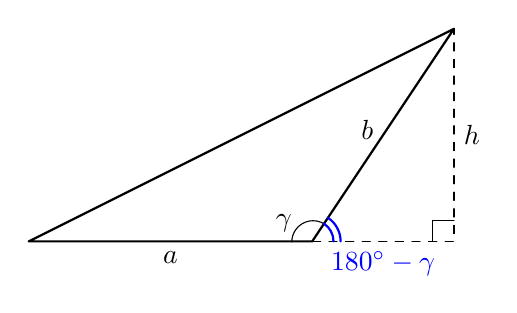
\begin{tikzpicture}[line cap=round,line join=round,>=triangle 45,x=0.9cm,y=0.9cm]
\draw [thick] (0,0)--(2,3)--(-4,0)--cycle;
\draw (1.7,0)--(1.7,0.3)--(2,0.3);
\draw [dashed] (0,0)--(2,0)--(2,3);
\draw  (53.6:0.3) arc (56.3:180:0.3); 
\node [left] at (120:0.3) {$\gamma$};
\node[above left] at (1,1.3) {$b$};
\node[below] at (-2,0) {$a$};
\node[right] at (2,1.5) {$h$};
\draw [thick, color = blue] (0:0.3) arc (0:56.3:0.3); 
\draw [thick, color = blue] (0:0.4) arc (0:56.3:0.4); 
\node [below, color = blue] at (1,0) {$180^\circ-\gamma$};
\end{tikzpicture}
\end{figurehere}
\end{center}

% kuva 44: Kolmion pinta-ala sinin avulla 2

\begin{center}
\begin{figurehere}
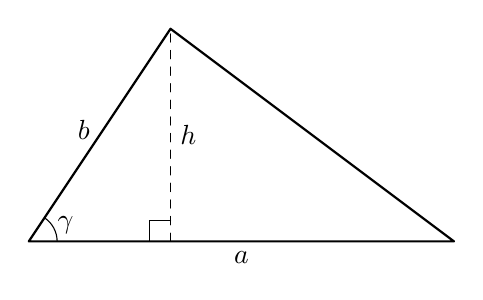
\begin{tikzpicture}[line cap=round,line join=round,>=triangle 45,x=0.9cm,y=0.9cm]
\draw [thick] (0,0)--(2,3)--(6,0)--cycle;
\draw (1.7,0)--(1.7,0.3)--(2,0.3);
\draw [dashed] (2,0)--(2,3);
%\draw  (53.6:0.3) arc (56.3:180:0.3); 
%\node [left] at (120:0.3) {$\gamma$};
\node[above left] at (1,1.3) {$b$};
\node[below] at (3,0) {$a$};
\node[right] at (2,1.5) {$h$};
\draw (0:0.4) arc (0:56.3:0.4); 
\node [right] at (40:0.35) {$\gamma$};
\end{tikzpicture}
\end{figurehere}
\end{center}

% kuva 45: Kolmion pinta-ala sinin avulla 3

\begin{center}
\begin{figurehere}
\begin{tikzpicture}[line cap=round,line join=round,>=triangle 45,x=0.9cm,y=0.9cm]
\draw [thick] (0,0)--(2,3)--(2,0)--cycle;
\draw (1.7,0)--(1.7,0.3)--(2,0.3);
%\draw [dashed] (2,0)--(2,3);
%\draw  (53.6:0.3) arc (56.3:180:0.3); 
%\node [left] at (120:0.3) {$\gamma$};
\node[above left] at (1,1.3) {$b$};
\node[below] at (1,0) {$a$};
\node[right] at (2,1.5) {$h$};
\draw (0:0.4) arc (0:56.3:0.4); 
\node [right] at (40:0.35) {$\gamma$};
\end{tikzpicture}
\end{figurehere}
\end{center}

% kuva 46: Kolmion pinta-ala sinin avulla 4

\begin{center}
\begin{figurehere}
\begin{tikzpicture}[line cap=round,line join=round,>=triangle 45,x=0.9cm,y=0.9cm]
\draw [thick] (0,0)--(2,3)--(-4,0)--cycle;
%\draw (1.7,0)--(1.7,0.3)--(2,0.3);
%\draw [dashed] (0,0)--(2,0)--(2,3);
\draw  (53.6:0.3) arc (56.3:180:0.3); 
\node [left] at (120:0.3) {$\gamma$};
\node[above left] at (1,1.3) {$b$};
\node[below] at (-2,0) {$a$};
%\node[right] at (2,1.5) {$h$};
%\draw [thick, color = blue] (0:0.3) arc (0:56.3:0.3); 
%\draw [thick, color = blue] (0:0.4) arc (0:56.3:0.4); 
%\node [below, color = blue] at (1,0) {$180^\circ-\gamma$};
\end{tikzpicture}
\end{figurehere}
\end{center}

% kuva 47: Suunnikkaan pinta-ala

\begin{center}
\begin{figurehere}
\begin{tikzpicture}[line cap=round,line join=round,>=triangle 45,x=0.9cm,y=0.9cm]
\draw [thick] (0,0)--(5,0)--(6.56,3.68)--(1.56,3.68)--cycle;
%\draw (1.7,0)--(1.7,0.3)--(2,0.3);
%\draw [dashed] (0,0)--(2,0)--(2,3);
\draw  (0:0.4) arc (0:67:0.4); 
\node [above right] at (30:0.35) {$67^\circ$};
\node[above left] at (0.75,1.8) {$4$};
\node[below] at (2.5,0) {$5$};
%\node[right] at (2,1.5) {$h$};
%\draw [thick, color = blue] (0:0.3) arc (0:56.3:0.3); 
%\draw [thick, color = blue] (0:0.4) arc (0:56.3:0.4); 
%\node [below, color = blue] at (1,0) {$180^\circ-\gamma$};
\end{tikzpicture}
\end{figurehere}
\end{center}

% kuva 48: Pythagoras ennen kosinilausetta

\begin{center}
\begin{figurehere}
\begin{tikzpicture}[line cap=round,line join=round,>=triangle 45,x=0.7cm,y=0.7cm]
\draw (0,0)--(4,0)--(0,3)--cycle;
\draw (0.3,0)--(0.3,0.3)--(0,0.3);
\node[below] at (2,0) {$b$};
\node[left] at (0,1.5) {$a$};
\node[above right] at (2,1.5) {$c$};
\node[above right] at (0.15,0.15) {$\gamma$};
\end{tikzpicture}
\end{figurehere}
\end{center}

% kuva 49: Kosinilauseen johtoa

\begin{center}
\begin{figurehere}
\begin{tikzpicture}[line cap=round,line join=round,>=triangle 45,x=0.9cm,y=0.9cm]
\draw [thick] (0,0)--(2,3)--(6,0)--cycle;
%\draw (1.7,0)--(1.7,0.3)--(2,0.3);
%\draw [dashed] (2,0)--(2,3);
\node[above left] at (1,1.3) {$b$};
\node[below] at (3,0) {$a$};
%\node[right] at (2,1.5) {$h$};
\node[above right] at (3.9,1.5) {$c$};
\draw (0:0.4) arc (0:56.3:0.4); 
\node [right] at (40:0.35) {$\gamma$};
\end{tikzpicture}
\end{figurehere}
\end{center}

% kuva 50: Kosinilauseen johtoa 2

\begin{center}
\begin{figurehere}
\begin{tikzpicture}[line cap=round,line join=round,>=triangle 45,x=0.9cm,y=0.9cm]
\draw [thick] (0,0)--(2,3)--(6,0)--cycle;
\draw (1.7,0)--(1.7,0.3)--(2,0.3);
\draw [dashed] (2,0)--(2,3);
\node[above left] at (1,1.3) {$b$};
%\node[below] at (3,0) {$a$};
\node[right] at (2,1.5) {$h$};
\node[above right] at (3.9,1.5) {$c$};
\draw (0:0.4) arc (0:56.3:0.4); 
\node [right] at (40:0.35) {$\gamma$};
\draw [decorate,decoration={brace,mirror, amplitude=8pt},xshift=0pt,yshift=-2pt] (0,0) -- (2,0) node [black,midway,yshift=-14pt] {$x$};
\draw [decorate,decoration={brace,mirror, amplitude=8pt},xshift=0pt,yshift=-2pt] (2,0) -- (6,0) node [black,midway,yshift=-14pt] {$a-x$};
\end{tikzpicture}
\end{figurehere}
\end{center}

% kuva 51: Kosinilauseen johtoa 3

\begin{center}
\begin{figurehere}
\begin{tikzpicture}[line cap=round,line join=round,>=triangle 45,x=0.9cm,y=0.9cm]
\draw [thick] (0,0)--(2,3)--(-4,0)--cycle;
\draw (1.7,0)--(1.7,0.3)--(2,0.3);
\draw [dashed] (0,0)--(2,0)--(2,3);
\draw  (53.6:0.3) arc (56.3:180:0.3); 
\node [left] at (120:0.3) {$\gamma$};
\node[above left] at (1,1.3) {$b$};
\node[below] at (-2,0) {$a$};
\node[below] at (1,0) {$x$};
\node[above left] at (-0.9,1.5) {$c$};
\node[right] at (2,1.5) {$h$};
\draw [thick, color = blue] (0:0.3) arc (0:56.3:0.3); 
\draw [thick, color = blue] (0:0.4) arc (0:56.3:0.4); 
\node [above, color = blue] at (1,0) {$\scriptstyle{180^\circ-\gamma}$};
\end{tikzpicture}
\end{figurehere}
\end{center}

% kuva 52: Kosinilauseen sovellus suunnikkaan lävistäjään

\begin{center}
\begin{figurehere}
\begin{tikzpicture}[line cap=round,line join=round,>=triangle 45,x=0.6cm,y=0.6cm]
\draw [thick] (2.87,4.01)--(0,0)--(8,0)--(10.87,4.01)--cycle;
%\draw (1.7,0)--(1.7,0.3)--(2,0.3);
%\draw [dashed] (2.87,4.01)--(8,0);
\draw  (0:0.6) arc (0:55:0.6); 
\node [right] at (40:0.6) {$55^\circ$};
\node[above left] at (1.4,2) {$5$};
\node[below] at (4,0) {$8$};
%\node[below] at (1,0) {$x$};
%\node[above left] at (-0.9,1.5) {$c$};
%\node[right] at (2,1.5) {$h$};
%\draw [thick, color = blue] (0:0.3) arc (0:56.3:0.3); 
%\draw [thick, color = blue] (0:0.4) arc (0:56.3:0.4); 
%\node [above, color = blue] at (1,0) {$\scriptstyle{180^\circ-\gamma}$};
\end{tikzpicture}
\end{figurehere}
\end{center}

% kuva 53: Kosinilauseen sovellus suunnikkaan lävistäjään 2

\begin{center}
\begin{figurehere}
\begin{tikzpicture}[line cap=round,line join=round,>=triangle 45,x=0.6cm,y=0.6cm]
\draw [thick] (2.87,4.01)--(0,0)--(8,0)--(10.87,4.01)--cycle;
%\draw (1.7,0)--(1.7,0.3)--(2,0.3);
\draw [dashed] (2.87,4.01)--(8,0);
\draw  (0:0.6) arc (0:55:0.6); 
\node [right] at (40:0.6) {$55^\circ$};
\node[above left] at (1.4,2) {$5$};
\node[below] at (4,0) {$8$};
%\node[below] at (1,0) {$x$};
%\node[above left] at (-0.9,1.5) {$c$};
%\node[right] at (2,1.5) {$h$};
%\draw [thick, color = blue] (0:0.3) arc (0:56.3:0.3); 
%\draw [thick, color = blue] (0:0.4) arc (0:56.3:0.4); 
%\node [above, color = blue] at (1,0) {$\scriptstyle{180^\circ-\gamma}$};
\end{tikzpicture}
\end{figurehere}
\end{center}

% kuva 54: Kosinilauseen sovellus suunnikkaan lävistäjään 3

\begin{center}
\begin{figurehere}
\begin{tikzpicture}[line cap=round,line join=round,>=triangle 45,x=0.6cm,y=0.6cm]
\draw [thick] (2.87,4.01)--(0,0)--(8,0)--(10.87,4.01)--cycle;
%\draw (1.7,0)--(1.7,0.3)--(2,0.3);
\draw [dashed] (0,0)--(10.87,4.01);
\begin{scope}[shift ={(8,0)}]
\draw  (55:0.45) arc (55:180:0.45); 
\node [above left] at (130:0.35) {$\gamma$};
\end{scope}
\node[above left] at (1.4,2) {$5$};
\node[below] at (4,0) {$8$};
%\node[below] at (1,0) {$x$};
%\node[above left] at (-0.9,1.5) {$c$};
%\node[right] at (2,1.5) {$h$};
%\draw [thick, color = blue] (0:0.3) arc (0:56.3:0.3); 
%\draw [thick, color = blue] (0:0.4) arc (0:56.3:0.4); 
%\node [above, color = blue] at (1,0) {$\scriptstyle{180^\circ-\gamma}$};
\end{tikzpicture}
\end{figurehere}
\end{center}

% kuva 55: Perus-Pythagoras tehtävään 1

\begin{center}
\begin{figurehere}
\begin{tikzpicture}[line cap=round,line join=round,>=triangle 45,x=0.9cm,y=0.9cm]
\draw [thick] (0,0)--(3.5,0)--(0,2.25)--cycle;
\draw (0.3,0)--(0.3,0.3)--(0,0.3);
\node[left] at (0,1.125) {$5$};
\node[below] at (1.75,0) {$7$};
\node[above right] at (1.75,1.125) {$x$};
\end{tikzpicture}
\end{figurehere}
\end{center}

% kuva 56: Perus-Pythagoras tehtävään 2

\begin{center}
\begin{figurehere}
\begin{tikzpicture}[line cap=round,line join=round,>=triangle 45,x=0.9cm,y=0.9cm]
\draw [thick] (0,0)--(0,3.1)--(7,3.1)--cycle;
\draw (0.3,3.1)--(0.3,2.8)--(0,2.8);
\node[left] at (0,1.5) {$6{,}2$ cm};
\node[below right] at (3.5,1.55) {$15{,}0$ cm};
\end{tikzpicture}
\end{figurehere}
\end{center}

% kuva 57: Kulmatehtävä

\begin{center}
\begin{figurehere}
\begin{tikzpicture}[line cap=round,line join=round,>=triangle 45,x=0.7cm,y=0.7cm]
\draw [thick] (-23:3)--(157:3);
\draw [thick] (20:3)--(200:3);
\draw  (200:0.4) arc (200:337:0.4); 
\node [below] at (270:0.35) {$137^\circ$};
\draw  (20:0.4) arc (20:157:0.4); 
\node [above] at (90:0.35) {$\beta$};
\draw  (157:0.55) arc (157:200:0.55); 
\node [left] at (180:0.5) {$\alpha$};
\end{tikzpicture}
\end{figurehere}
\end{center}

% kuva 58: Kulmatehtävä

\begin{center}
\begin{figurehere}
\begin{tikzpicture}[line cap=round,line join=round,>=triangle 45,x=1cm,y=1cm]
\draw [thick] (-1,0)--(4,0);
\draw [thick] (-1,2)--(4,2);
\draw [thick] (0,0)--(2.65,2);
\draw  (0:0.5) arc (0:37:0.5); 
\node [right] at (27:0.45) {$37^\circ$};
\begin{scope}[shift = {(2.65,2)}]
\draw  (180:0.5) arc (180:217:0.5); 
\node [left] at (207:0.45) {$\alpha$};
\draw  (217:0.3) arc (217:360:0.3); 
\node [below right] at (315:0.15) {$\beta$};
\end{scope}
\node [below] at (-0.5,0) {$L_2$};
\node [above] at (-0.5,2) {$L_1$};
\end{tikzpicture}
\end{figurehere}
\end{center}

% kuva 59: Kulmatehtävä 2

\begin{center}
\begin{figurehere}
\begin{tikzpicture}[line cap=round,line join=round,>=triangle 45,x=0.7cm,y=0.7cm]
\draw [thick] (180:3)--(0:3);
\draw [thick] (146:3)--(326:3);
\draw [thick] (0,0)--(27:3);
\draw  (180:0.4) arc (180:326:0.4); 
\node [below] at (270:0.35) {$146^\circ$};
\draw  (27:0.4) arc (27:146:0.4); 
\node [above] at (90:0.35) {$\alpha$};
\draw  (0:0.6) arc (0:27:0.6); 
\node [right] at (22:0.55) {\scriptsize{$27^\circ$}};
\end{tikzpicture}
\end{figurehere}
\end{center}

% kuva 59: Kulmakolmiotehtävä

\begin{center}
\begin{figurehere}
\begin{tikzpicture}[line cap=round,line join=round,>=triangle 45,x=1cm,y=1cm]
\draw [thick] (0,0)--(0,2.89)--(5,0)--cycle;
\draw [thick] (0,0)--(3,1.15)--(3,0);
\draw (0,0.2)--(0.2,0.2)--(0.2,0);
\draw (2.85,0)--(2.85,0.15)--(3,0.15);
\draw  (21.1:0.4) arc (21.1:90:0.4); 
\node [above right] at (70:0.3) {\scriptsize{$68{,}9^\circ$}};
\begin{scope}[shift = {(3,1.15)}]
\draw  (150:0.4) arc (150:201.1:0.4); 
\node [left] at (180:0.35) {$\beta$};
\draw  (201.1:0.3) arc (201.1:270:0.3); 
\node [below left] at (240:0.15) {$\gamma$};
\draw  (270:0.4) arc (270:330:0.4); 
\node [below right] at (300:0.2) {$\delta$};
\end{scope}
\begin{scope}[shift = {(0,2.89)}]
\draw  (270:0.4) arc (270:330:0.4); 
\node [below] at (320:0.45) {\scriptsize{$60^\circ$}};
\end{scope}
\end{tikzpicture}
\end{figurehere}
\end{center}

% kuva 60: Tasakylkinen kolmio

\begin{center}
\begin{figurehere}
\begin{tikzpicture}[line cap=round,line join=round,>=triangle 45,x=1cm,y=1cm]
\draw [thick] (0,0)--(2,0)--(1,3)--cycle;
\draw [dashed] (1,3)--(1,0);
\draw (1,0.15)--(1.15,0.15)--(1.15,0);
\node [above left] at (0.5,1.5) {$s$};
\node [above right] at (1.5,1.5) {$s$};
\draw  (0:0.3) arc (0:71.57:0.3); 
\begin{scope}[shift = {(2,0)}]
\draw  (108.43:0.3) arc (108.43:180:0.3); 
\end{scope}
\end{tikzpicture}
\end{figurehere}
\end{center}

% kuva 61: Prosenttisuorakulmio

\begin{center}
\begin{figurehere}
\begin{tikzpicture}[line cap=round,line join=round,>=triangle 45,x=1cm,y=1cm]
\draw [fill, color = LightSkyBlue] (0,0)--(4,1.5)--(3,0)--cycle;
\draw [thick] (0,0)--(4,0)--(4,1.5)--(0,1.5)--cycle;
\draw (0,0)--(4,1.5)--(3,0);
\node [below] at (1.5,0) {$3a$};
\node [below] at (3.5,0) {$a$};
\end{tikzpicture}
\end{figurehere}
\end{center}

% kuva 62: Sänky

\begin{center}
\begin{figurehere}
\begin{tikzpicture}[line cap=round,line join=round,>=triangle 45,x=1cm,y=1cm]
\draw [thick] (0,0)--(4,0)--(4,2)--(0,2)--cycle;
\draw [fill, color = Lavender] (0.05,0.05)--(0.95,0.05)--(0.95,1.79)--(0.05,1.79)--cycle;
\draw (0.05,0.05)--(0.95,0.05)--(0.95,1.79)--(0.05,1.79)--cycle;
\end{tikzpicture}
\end{figurehere}
\end{center}

% kuva 63: Sänky

\begin{center}
\begin{figurehere}
\begin{tikzpicture}[line cap=round,line join=round,>=triangle 45,x=1cm,y=1cm]
\draw [thick] (0,0)--(4,0)--(4,2)--(0,2)--cycle;
\draw [fill, color = Lavender] (0.05,0.05)--(1.79,0.05)--(1.79,0.95)--(0.05,0.95)--cycle;
\draw (0.05,0.05)--(1.79,0.05)--(1.79,0.95)--(0.05,0.95)--cycle;
\end{tikzpicture}
\end{figurehere}
\end{center}

% kuva 64: Lattialista

\begin{center}
\begin{figurehere}
\begin{tikzpicture}[line cap=round,line join=round,>=triangle 45,x=1cm,y=1cm]
\draw (0,0)--(-4,2)--(-3.5,3)--(0.5,1)--cycle;
\draw [thick] (-4,3.5)--(-4,0)--(0.5,0)--(0.5,3.5);
\end{tikzpicture}
\end{figurehere}
\end{center}

% kuva 65: Kulma koordinaatistossa -tehtävä

\begin{center}
\begin{figurehere}
\begin{tikzpicture}[line cap=round,line join=round,>=triangle 45,x=2.5cm,y=2.5cm]
\draw[->,color=gray] (-1.5,0) -- (1.5,0);
%tiksut ja viivat
\foreach \x in {-1,1}
{
\draw[shift={(\x,0)},color=black] (0pt,2pt) -- (0pt,-2pt);
}
\node [below] at (1.5,0) {$x$};

%y-akseli
\draw[->,color=gray] (0,-0.5) -- (0,1.5);
%tiksut ja viivat
\foreach \y in {-1,1}
{
\draw[shift={(0,\y)},color=black] (2pt,0pt) -- (-2pt,0pt);
}
\node [left] at (0,1.5) {$y$};
\begin{scope}
\clip (-1,0)--(1,0)--(1,1)--(-1,1)--cycle;
\draw[color = gray] (0,0) circle [radius = 1];
\end{scope}
\node [below] at (-1.05,-0.05) {$-1$};
\node [below] at (1,-0.05) {$1$};
\draw [thick] (1,0)--(0,0) -- (152:1);
\draw [fill] (152:1) circle [radius = 1.2pt];
\draw (0:0.15) arc (0:152:0.15); 
\node [right] at (60:0.19) {$152^\circ$};
\node [left] at (152:1) {$A$};
\end{tikzpicture}
\end{figurehere}
\end{center}

% kuva 66: Joki

\begin{center}
\begin{figurehere}
\begin{tikzpicture}[line cap=round,line join=round,>=triangle 45,x=0.8cm,y=0.8cm]
\draw [fill, color = AliceBlue] (-0.5,0)--(9.5,0)--(9.5,2)--(-0.5,2)--cycle;
\draw [thick] (-0.5,0)--(9.5,0);
\draw [thick] (-0.5,2)--(9.5,2);
\draw (0,0)--(55:2.44);
\draw (0:0.3) arc (0:55:0.3);
\node [right] at (45:0.3) {\scriptsize{$55^\circ$}};
\node [below] at (4.43,0) {\scriptsize{$450 \text{ m}$}};
\begin{scope}[shift={(1.4,2)}]
\draw (0,0)--(-15:7.73);
\end{scope}
\begin{scope}[shift={(8.86,0)}]
\draw (165:1.2) arc (165:180:1.2);
\node [left] at (171:1.2) {\scriptsize{$15^\circ$}};
\end{scope}
\end{tikzpicture}
\end{figurehere}
\end{center}

% kuva 67: Kiekonheitto

\begin{center}
\begin{figurehere}
\begin{tikzpicture}[line cap=round,line join=round,>=triangle 45,x=1cm,y=1cm]
\draw [fill, color = PaleGreen] (-17.46:6)--(0,0)--(17.46:6)--cycle;
\draw [fill, color = white] (0,0) circle [radius = 0.5];
\draw (-17.46:6)--(0,0)--(17.46:6);
\draw (0,0) circle [radius = 0.5];
\draw [thick] (0,0)--(3,-2)--(5,-0.5);
\draw [fill] (0,0) circle [radius = 1pt];
\draw [fill] (3,-2) circle [radius = 1pt];
\draw [fill] (5,-0.5) circle [radius = 1pt];
\node [above] at (5,-0.5) {$C$};
\node [below] at (3,-2) {$A$};
\node [above] at (0,0) {$B$};
\begin{scope}[shift={(3,-2)}]
\draw (36.87:0.3) arc (36.87:146.31:0.3);
%\node [above] at (90:0.3) {};
\end{scope}
\end{tikzpicture}
\end{figurehere}
\end{center}

% kuva 68: Kulmanpuolittajalause-tehtävä

\begin{center}
\begin{figurehere}
\begin{tikzpicture}[line cap=round,line join=round,>=triangle 45,x=1cm,y=1cm]
\draw [thick] (60:3)--(0,0)--(6,0)--cycle;
\draw (0,0)--(3,1.732);
\node [left] at (0,0) {$A$};
\node [right] at (6,0) {$B$};
\node [above] at (1.5,2.598) {$C$};
\node [above right] at (3,1.732) {$D$};
\draw (0:0.5) arc (0:30:0.5);
\draw (30:0.6) arc (30:60:0.6);
\draw (15:0.42)--(15:0.58);
\draw (45:0.52)--(45:0.68);
\end{tikzpicture}
\end{figurehere}
\end{center}

% kuva 69: Yhdenmuotoisuus

\begin{center}
\begin{figurehere}
\begin{tikzpicture}[line cap=round,line join=round,>=triangle 45,x=1cm,y=1cm]
\draw [thick] (0,0.25)--(2,0.25)--(2,1)--(3,0)--(2,-1)--(2,-0.25)--(0,-0.25)--cycle;
\begin{scope}[shift={(4,0)}, scale=0.5]
\draw [thick] (0,0.25)--(2,0.25)--(2,1)--(3,0)--(2,-1)--(2,-0.25)--(0,-0.25)--cycle;
\end{scope}
\begin{scope}[shift={(6.5,-0.5)}, scale=0.5, rotate=45]
\draw [thick] (0,0.25)--(2,0.25)--(2,1)--(3,0)--(2,-1)--(2,-0.25)--(0,-0.25)--cycle;
\end{scope}
\begin{scope}[shift={(9.5,-0.5)}, scale=0.5, rotate=135]
\draw [thick] (0,0.25)--(2,0.25)--(2,1)--(3,0)--(2,-1)--(2,-0.25)--(0,-0.25)--cycle;
\end{scope}
\draw[dashed] (8,-1)--(8,1);
\node [above] at (4.5, 0.8) {$\text{pienenn\"{o}s}$};
\node [above] at (7, 0.8) {$\text{kierto}\phantom{p}$};
\node [above] at (8.8, 0.8) {$\text{peilaus}$};
\end{tikzpicture}
\end{figurehere}
\end{center}

% kuva 70: Suunnikkaan pinta-ala

\begin{center}
\begin{figurehere}
\begin{tikzpicture}[line cap=round,line join=round,>=triangle 45,x=1cm,y=1cm]
\draw [thick] (0,0)--(5,0)--(7,2)--(2,2)--cycle;
\draw [dashed] (2,2)--(2,0);
\draw (2.2,0)--(2.2,0.2)--(2,0.2);
\node [below] at (2.5,0) {$a$};
\node [right] at (2,1) {$h$};
\end{tikzpicture}
\end{figurehere}
\end{center}

% kuva 71: Puolisuunnikkaan pinta-ala

\begin{center}
\begin{figurehere}
\begin{tikzpicture}[line cap=round,line join=round,>=triangle 45,x=1cm,y=1cm]
\draw [thick] (0,0)--(5,0)--(2,2)--(-1,2)--cycle;
\draw [dashed] (0,2)--(0,0);
\draw (0.2,0)--(0.2,0.2)--(0,0.2);
\node [below] at (2.5,0) {$a$};
\node [right] at (0,1) {$h$};
\node [above] at (0.5,2) {$b$};
\end{tikzpicture}
\end{figurehere}
\end{center}

% kuva 72: Suunnikkaan pinta-ala

\begin{center}
\begin{figurehere}
\begin{tikzpicture}[line cap=round,line join=round,>=triangle 45,x=1cm,y=1cm]
\draw [thick] (0,0)--(2,0)--(-1,2)--(-3,2)--cycle;
\draw [dashed] (-3,2)--(-3,0)--(0,0);
\draw (-2.8,0)--(-2.8,0.2)--(-3,0.2);
\node [below] at (1,0) {$a$};
\node [left] at (-3,1) {$h$};
%\node [above] at (0.5,2) {$b$};
\end{tikzpicture}
\end{figurehere}
\end{center}

% kuva 73: Puolisuunnikkaan pinta-ala

\begin{center}
\begin{figurehere}
\begin{tikzpicture}[line cap=round,line join=round,>=triangle 45,x=1cm,y=1cm]
\draw [thick] (0,0)--(3,0)--(-1,2)--(-2,2)--cycle;
\draw [dashed] (-2,2)--(-2,0)--(0,0);
\draw (-1.8,0)--(-1.8,0.2)--(-2,0.2);
\node [below] at (1.3,0) {$a$};
\node [left] at (-2,1) {$h$};
\node [above] at (-1.5,2) {$b$};
\end{tikzpicture}
\end{figurehere}
\end{center}

% kuva 74: Puolisuunnikkaan pinta-ala

\begin{center}
\begin{figurehere}
\begin{tikzpicture}[line cap=round,line join=round,>=triangle 45,x=1cm,y=1cm]
\draw [fill, color = LightSkyBlue] (0,0)--(3,0)--(-2,2)--cycle;
\draw [fill, color = LightPink] (3,0)--(-1,2)--(-2,2)--cycle;
\draw (3,0)--(-2,2);
\draw [thick] (0,0)--(3,0)--(-1,2)--(-2,2)--cycle;
\draw [dashed] (-2,2)--(-2,0)--(0,0);
\draw (-1.8,0)--(-1.8,0.2)--(-2,0.2);
\draw [dashed] (-1,2)--(3,2)--(3,0);
\draw (2.8,2)--(2.8,1.8)--(3,1.8);
\node [below] at (1.3,0) {$a$};
\node [left] at (-2,1) {$h$};
\node [right] at (3,1) {$h$};
\node [above] at (-1.5,2) {$b$};
\end{tikzpicture}
\end{figurehere}
\end{center}

% kuva 74: Yhdenmuotoisuus

\begin{center}
\begin{figurehere}
\begin{tikzpicture}[line cap=round,line join=round,>=triangle 45,x=1.5cm,y=1.5cm]
\draw [fill, color = Gold] (30:2)--(150:2)--(270:2)--cycle;
\draw [fill, color = Gold] (-30:2)--(90:2)--(210:2)--cycle;
\draw (30:2)--(60:1.155)--(90:2)--(120:1.155)--(150:2)--(180:1.155)--(210:2)--(240:1.155)--(270:2)--(300:1.155)--(330:2)--(360:1.155)--cycle;
\node [above] at (1.155,1) {$2 \text{ cm}$};
\begin{scope}[shift={(3,0)}, scale=0.25]
\draw [fill, color = Gold] (30:2)--(150:2)--(270:2)--cycle;
\draw [fill, color = Gold] (-30:2)--(90:2)--(210:2)--cycle;
\draw (30:2)--(60:1.155)--(90:2)--(120:1.155)--(150:2)--(180:1.155)--(210:2)--(240:1.155)--(270:2)--(300:1.155)--(330:2)--(360:1.155)--cycle;
\node [above] at (1.6,0.9) {\scriptsize{$0{,}5 \text{ cm}$}};
\end{scope}
\end{tikzpicture}
\end{figurehere}
\end{center}

% kuva 74: Yhdenmuotoisuus ja pinta-ala

\begin{center}
\begin{figurehere}
\begin{tikzpicture}[line cap=round,line join=round,>=triangle 45,x=0.7cm,y=0.7cm]
\draw [fill, color = Plum] (0,0)--(2.5,0)--(2.5,1)--(0,1)--cycle;
\draw (0,0)--(2.5,0)--(2.5,1)--(0,1)--cycle;
\node [below] at (1.5,0) {$2{,}5 \text{ cm}$};
\node [left] at (0,0.5) {$1 \text{ cm}$};
\begin{scope}[shift={(0,2)}, scale=3]
\draw [fill, color = Plum] (0,0)--(2.5,0)--(2.5,1)--(0,1)--cycle;
\draw (0,0)--(2.5,0)--(2.5,1)--(0,1)--cycle;
%\node [below] at (1.5,0) {$3 \text{ cm}$};
\node [left] at (0,0.5) {$3 \text{ cm}$};
\end{scope}
\end{tikzpicture}
\end{figurehere}
\end{center}

% kuva 75: Yhdenmuotoisuus ja pinta-ala

\begin{center}
\begin{figurehere}
\begin{tikzpicture}[line cap=round,line join=round,>=triangle 45,x=0.5cm,y=0.5cm]
%\draw [fill, color = PaleGreen] (0,0)--(6,0)--(6,3)--(0,3)--cycle;
\draw [thick] (0,0)--(6,0)--(6,3)--(0,3)--cycle;
%\node [below] at (3,0) {$3a$};
%\node [left] at (0,1.5) {$3b$};
%\foreach \x in {1,2}
%{\draw[dashed] (2*\x,0)--(2*\x,3);
%\draw[dashed] (0, \x)--(6,\x);
%}
\begin{scope}[shift={(0,4)}, scale=5/3]
%\draw [fill, color = PaleGreen] (0,0)--(6,0)--(6,3)--(0,3)--cycle;
\draw [thick] (0,0)--(6,0)--(6,3)--(0,3)--cycle;
%\node [below] at (3,0) {$3a$};
%\node [left] at (0,1.5) {$3b$};
\end{scope}
\end{tikzpicture}
\end{figurehere}
\end{center}

% kuva 76: Yhdenmuotoisuus ja pinta-ala

\begin{center}
\begin{figurehere}
\begin{tikzpicture}[line cap=round,line join=round,>=triangle 45,x=0.5cm,y=0.5cm]
%\draw [fill, color = PaleGreen] (0,0)--(6,0)--(6,3)--(0,3)--cycle;
\draw [thick] (0,0)--(6,0)--(6,3)--(0,3)--cycle;
\node [below] at (3,0) {$3a$};
\node [left] at (0,1.5) {$3b$};
\foreach \x in {1,2}
{\draw (2*\x,0)--(2*\x,3);
\draw (0, \x)--(6,\x);
}
\end{tikzpicture}
\end{figurehere}
\end{center}

% kuva 77: Pellon pinta-ala

\begin{center}
\begin{figurehere}
\begin{tikzpicture}[line cap=round,line join=round,>=triangle 45,x=1cm,y=1cm]
\draw [fill, color = LightGoldenrod] (0,0)--(3.6,0)--(3.6,-2.8)--(-150:3.2)--cycle;
\draw [thick] (0,0)--(3.6,0)--(3.6,-2.8)--(-150:3.2)--cycle;
\draw (3.3,0)--(3.3,-0.3)--(3.6,-0.3);
\draw (-150:0.3) arc (-150:0:0.3);
\node [above] at (1.8,0) {$360 \text{ m}$};
\node [right] at (3.6,-1.4) {$280 \text{ m}$};
\node [below] at (-80:0.3) {$150^\circ$};
\path (-150:3.2)--(0,0) node [midway, above left] {$320 \text{ m}$};
%\foreach \x in {1,2}
%{\draw (2*\x,0)--(2*\x,3);
%\draw (0, \x)--(6,\x);
%}
\end{tikzpicture}
\end{figurehere}
\end{center}


% kuva 78: Nelikulmiot

\begin{center}
\begin{figurehere}
\begin{tikzpicture}[line cap=round,line join=round,>=triangle 45,x=0.7cm,y=0.7cm]
\draw [thick] (0,0)--(0,4)--(1,2)--(4,3)--cycle;
\draw [thick] (5,2)--(6,0)--(9,2)--(6,3)--cycle;
\end{tikzpicture}
\end{figurehere}
\end{center}

% kuva 79: Kuusikulmio

\begin{center}
\begin{figurehere}
\begin{tikzpicture}[line cap=round,line join=round,>=triangle 45,x=0.7cm,y=0.7cm]
\draw[help lines,step=1, dashed, color = gray] (0,0) grid (5,5);
\draw [thick] (1,1)--(3,2)--(3,1)--(4,4)--(2,3)--(2,4)--cycle;
\end{tikzpicture}
\end{figurehere}
\end{center}

% kuva 80: Tasasivuinen kolmio

\begin{center}
\begin{figurehere}
\begin{tikzpicture}[line cap=round,line join=round,>=triangle 45,x=0.7cm,y=0.7cm]
\begin{scope}
\clip (-1,1)--(-1,6)--(6,6)--(6,1)--cycle;
\draw [color = Gray] (0,0) circle [radius = 5];
\draw [color = Gray] (5,0) circle [radius = 5];
\end{scope}
\draw [thick] (0,0)--(5,0);
\draw [fill] (2.5, 4.33) circle [radius = 1.2pt];
\end{tikzpicture}
\end{figurehere}
\end{center}

% kuva 81: Tasasivuinen muistikolmio

\begin{center}
\begin{figurehere}
\begin{tikzpicture}[line cap=round,line join=round,>=triangle 45,x=0.7cm,y=0.7cm]
\begin{scope}[shift = {(2.5,4.33)}]
\draw (240:0.6) arc (240:270:0.6);
\node [below] at (245:0.6) {$\beta$};
\end{scope}
\draw [thick] (0,0)--(5,0)--(2.5, 4.33)--cycle;
\draw (2.5, 4.33)--(2.5,0);
\draw (2.2, 0)--(2.2,0.3)--(2.5,0.3);
\draw (0:0.4) arc (0:60:0.4);
\node [right] at (45:0.4) {$\alpha$};
\node [right] at (2.5,2.16) {$h$};
\path (0,0)--(2.5,4.33) node [midway, above left] {$2$};
\draw [decorate,decoration={brace,mirror, amplitude=8pt},xshift=0pt,yshift=-2pt] (0,0) -- (2.5,0) node [black,midway,yshift=-14pt] {$x$};
\end{tikzpicture}
\end{figurehere}
\end{center}

% kuva 82: Tasasivuinen muistikolmio

\begin{center}
\begin{figurehere}
\begin{tikzpicture}[line cap=round,line join=round,>=triangle 45,x=0.7cm,y=0.7cm]
\draw [thick] (0,0)--(5,0)--(2.5, 4.33)--cycle;
\draw (2.5, 4.33)--(2.5,0);
\draw (2.2, 0)--(2.2,0.3)--(2.5,0.3);
\node [above] at (2.5,4.33) {$C$};
\node [below] at (0,0) {$A$};
\node [below] at (5,0) {$B$};
\node [below] at (2.5,0) {$D$};
\end{tikzpicture}
\end{figurehere}
\end{center}

% kuva 83: Neliö

\begin{center}
\begin{figurehere}
\begin{tikzpicture}[line cap=round,line join=round,>=triangle 45,x=0.7cm,y=0.7cm]
%\begin{scope}[shift = {(2.5,4.33)}]
%\draw (240:0.6) arc (240:270:0.6);
%\node [below] at (245:0.6) {$\beta$};
%\end{scope}
\draw [thick] (0,0)--(4,0)--(4,4)--(0,4)--cycle;
\draw (0,0)--(4,4);
\draw (3.7, 0)--(3.7,0.3)--(4,0.3);
\draw (0:0.4) arc (0:45:0.4);
\node [right] at (40:0.4) {$\alpha$};
\node [right] at (4,2) {$1$};
\path (0,0)--(4,4) node [midway, above left] {$x$};
\node [below] at (2,0) {$1$};
%\draw [decorate,decoration={brace,mirror, amplitude=8pt},xshift=0pt,yshift=-2pt] (0,0) -- (2.5,0) node [black,midway,yshift=-14pt] {$x$};
\end{tikzpicture}
\end{figurehere}
\end{center}

% kuva 84: Säännöllisiä monikulmioita

\begin{center}
\begin{figurehere}
\begin{tikzpicture}[line cap=round,line join=round,>=triangle 45,x=0.7cm,y=0.7cm]
\draw [thick] (-30:1.5)--(90:1.5)--(210:1.5)--cycle;
\begin{scope}[shift = {(3.5,0)}]
\draw [thick] (-45:1.5)--(45:1.5)--(135:1.5)--(225:1.5)--cycle;
\end{scope}
\begin{scope}[shift = {(7,0)}]
\draw [thick] (18:1.5)--(90:1.5)--(162:1.5)--(234:1.5)--(306:1.5)--cycle;
\end{scope}
\begin{scope}[shift = {(10.5,0)}]
\draw [thick] (30:1.5)--(90:1.5)--(150:1.5)--(210:1.5)--(270:1.5)--(330:1.5)--cycle;
\end{scope}
\begin{scope}[shift = {(14,0)}]
\draw [thick] (38.57:1.5)--(90:1.5)--(141.43:1.5)--(192.86:1.5)--(244.29:1.5)--(295.71:1.5)--(347.14:1.5)--cycle;
\end{scope}
\end{tikzpicture}
\end{figurehere}
\end{center}

% kuva 85: Täyskulma

\begin{center}
\begin{figurehere}
\begin{tikzpicture}[line cap=round,line join=round,>=triangle 45,x=0.7cm,y=0.7cm]
\draw [thick] (0,0)--(3,0);
\draw (0:0.3) arc (0:360:0.3);
\draw [fill] (0,0) circle [radius = 1.2pt];
\end{tikzpicture}
\end{figurehere}
\end{center}

% kuva 86: Kuusikulmio 1

\begin{center}
\begin{figurehere}
\begin{tikzpicture}[line cap=round,line join=round,>=triangle 45,x=0.6cm,y=0.6cm]
\draw [color = Gray] (0,0) circle [radius = 3];
\draw [color = Gray] (0,0)--(3,0);
\draw [fill] (0,0) circle [radius = 1.2pt];
\draw [fill] (3,0) circle [radius = 1.2pt];
\end{tikzpicture}
\end{figurehere}
\end{center}

% kuva 86: Kuusikulmio 2

\begin{center}
\begin{figurehere}
\begin{tikzpicture}[line cap=round,line join=round,>=triangle 45,x=0.6cm,y=0.6cm]
\draw [color = Gray] (0,0) circle [radius = 3];
\draw [color = Gray] (0,0)--(3,0);
\draw [fill] (0,0) circle [radius = 1.2pt];
\draw [fill] (3,0) circle [radius = 1.2pt];
\draw [color = Gray] (0,0)--(72:3);
\draw [fill] (72:3) circle [radius = 1.2pt];
\end{tikzpicture}
\end{figurehere}
\end{center}

% kuva 86: Viisikulmio 3

\begin{center}
\begin{figurehere}
\begin{tikzpicture}[line cap=round,line join=round,>=triangle 45,x=0.6cm,y=0.6cm]
\draw [color = Gray] (0,0) circle [radius = 3];
\foreach  \x in {0,...,4}
{
\draw [color = Gray] (0,0)--(\x*72:3);
\draw [fill] (\x*72:3) circle [radius = 1.2pt];
}
\draw [fill] (0,0) circle [radius = 1.2pt];
\end{tikzpicture}
\end{figurehere}
\end{center}

% kuva 87: Ympyrän määritelmä

\begin{center}
\begin{figurehere}
\begin{tikzpicture}[line cap=round,line join=round,>=triangle 45,x=0.6cm,y=0.6cm]
\draw [thick] (0,0) circle [radius = 2];
\draw [color = DarkSlateGray] (0,0)--(72:2);
\draw [fill] (0,0) circle [radius = 1.1pt];
\node [below] at (0,0) {\scriptsize{keskipiste}};
\node [left] at (72:1) {\scriptsize{s\"{a}de}};
\end{tikzpicture}
\end{figurehere}
\end{center}

% kuva 88: Ympyrän määritelmä

\begin{center}
\begin{figurehere}
\begin{tikzpicture}[line cap=round,line join=round,>=triangle 45,x=0.6cm,y=0.6cm]
\draw [thick] (0,0) circle [radius = 2];
\draw [color = DarkSlateGray] (160:2)--(-20:2);
\draw [fill] (0,0) circle [radius = 1.1pt];
\draw [color = DarkSlateGray] (150:2)--(80:2);
\node [below left] at (-20:0.5) {\scriptsize{halkaisija}};
\path (150:2)--(80:2) node [midway, below right] {\scriptsize{j\"{a}nne}};
\end{tikzpicture}
\end{figurehere}
\end{center}

% kuva 89: Ympyrän kehän pituus

\begin{center}
\begin{figurehere}
\begin{tikzpicture}[line cap=round,line join=round,>=triangle 45,x=1cm,y=1cm]
\foreach  \x in {0,...,5}
{
\draw [color = Gray] (0,0)--(30+\x*60:1.5);
}
\draw [thick, color = red] (0,0) circle [radius=1.5];
\draw (30:1.5)--(90:1.5)--(150:1.5)--(210:1.5)--(270:1.5)--(330:1.5)--cycle;
\draw (30:1.732)--(90:1.732)--(150:1.732)--(210:1.732)--(270:1.732)--(330:1.732)--cycle;
%
\begin{scope}[shift = {(3.5,0)}]
\foreach  \x in {0,...,9}
{
\draw [color = Gray] (0,0)--(\x*36:1.5);
}
\draw [thick, color = red] (0,0) circle [radius=1.5];
\draw (36:1.5)--(72:1.5)--(108:1.5)--(144:1.5)--(180:1.5)--(216:1.5)--(252:1.5)--(288:1.5)--(324:1.5)--(360:1.5)--cycle;
\draw (36:1.577)--(72:1.577)--(108:1.577)--(144:1.577)--(180:1.577)--(216:1.577)--(252:1.577)--(288:1.577)--(324:1.577)--(360:1.577)--cycle;
\end{scope}
%
\begin{scope}[shift = {(7,0)}]
\foreach  \x in {0,...,19}
{
\draw [color = Gray] (0,0)--(\x*18:1.5);
}
\draw [thick, color = red] (0,0) circle [radius=1.5];
\draw (18:1.5)--(36:1.5)--(54:1.5)--(72:1.5)--(90:1.5)--(108:1.5)--(126:1.5)--(144:1.5)--(162:1.5)--(180:1.5)--(198:1.5)--(216:1.5)--(234:1.5)--(252:1.5)--(270:1.5)--(288:1.5)--(306:1.5)--(324:1.5)--(342:1.5)--(360:1.5)--cycle;
\draw (18:1.519)--(36:1.519)--(54:1.519)--(72:1.519)--(90:1.519)--(108:1.519)--(126:1.519)--(144:1.519)--(162:1.519)--(180:1.519)--(198:1.519)--(216:1.519)--(234:1.519)--(252:1.519)--(270:1.519)--(288:1.519)--(306:1.519)--(324:1.519)--(342:1.519)--(360:1.519)--cycle;
\end{scope}
\end{tikzpicture}
\end{figurehere}
\end{center}

% kuva 90: Luku pii

\begin{center}
\begin{figurehere}
\begin{tikzpicture}[line cap=round,line join=round,>=triangle 45,x=0.6cm,y=0.6cm]
\draw [thick] (0,0) circle [radius = 2];
\draw [color = DarkSlateGray] (180:2)--(0:2);
\draw [fill] (0,0) circle [radius = 1.1pt];
\node [below] at (0:0.5) {$d$};
\node [above right] at (45:2) {$p$};
\end{tikzpicture}
\end{figurehere}
\end{center}

% kuva 91: Ympyrän pinta-ala

\begin{center}
\begin{figurehere}
\begin{tikzpicture}[line cap=round,line join=round,>=triangle 45,x=1cm,y=1cm]
\draw [color = red] (0,0)--(0,1.5);
\foreach  \x in {1,...,15}
{
\draw (0,0) circle [radius = \x*0.1];
}
\draw [fill] (0,0) circle [radius = 1pt];
\end{tikzpicture}
\end{figurehere}
\end{center}

% kuva 92: Ympyrän pinta-ala 2

\begin{center}
\begin{figurehere}
\begin{tikzpicture}[line cap=round,line join=round,>=triangle 45,x=1cm,y=1cm]
\draw [dashed, color = DarkSlateGray] (0,0)--(9.425,1.5);
\draw [color = red] (0,0)--(0,1.5);
\foreach  \x in {1,...,15}
{
\draw (0,\x*0.1)--(0.6283*\x,\x*0.1);
}
\draw [fill] (0,0) circle [radius = 1pt];
\end{tikzpicture}
\end{figurehere}
\end{center}

% kuva 93: Keskuskulma

\begin{center}
\begin{figurehere}
\begin{tikzpicture}[line cap=round,line join=round,>=triangle 45,x=0.6cm,y=0.6cm]
\draw [thick] (0,0) circle [radius = 2];
\draw (35:2)--(0,0)--(-35:2);
\draw [fill] (0,0) circle [radius = 0.9pt];
\draw (-35:0.5) arc (-35:35:0.5);
\node [right] at (0:0.5) {$\alpha$};
%\node [above right] at (45:2) {$p$};
\end{tikzpicture}
\hspace{5mm}
\begin{tikzpicture}[line cap=round,line join=round,>=triangle 45,x=0.6cm,y=0.6cm]
\draw [thick] (0,0) circle [radius = 2];
\draw (35:2)--(-2,0)--(-35:2);
\draw [fill] (0,0) circle [radius = 0.9pt];
\begin{scope}[shift={(-2,0)}]
\draw (-17.5:0.9) arc (-17.5:17.5:0.9);
\node [right] at (0:0.9) {$\beta$};
\end{scope}
%\node [above right] at (45:2) {$p$};
\end{tikzpicture}
\end{figurehere}
\end{center}

% kuva 94: Sektori

\begin{center}
\begin{figurehere}
\begin{tikzpicture}[line cap=round,line join=round,>=triangle 45,x=0.6cm,y=0.6cm]
\begin{scope}
\clip (0,0) circle [radius = 2];
\draw [fill, color=PaleGreen] (55:4)--(0,0)--(-55:4)--cycle;
\end{scope}
\begin{scope}
\clip  (55:4)--(0,0)--(-55:4)--cycle;
\draw [very thick] (0,0) circle [radius = 2];
\end{scope}
\draw  (0,0) circle [radius = 2];
\draw (55:2)--(0,0)--(-55:2);
\draw [fill] (0,0) circle [radius = 0.9pt];
\draw (-55:0.5) arc (-55:55:0.5);
\node [right] at (0:0.5) {$\alpha$};
%\node [above right] at (45:2) {$p$};
\end{tikzpicture}
\hspace{5mm}
\begin{tikzpicture}[line cap=round,line join=round,>=triangle 45,x=0.6cm,y=0.6cm]
\begin{scope}
\clip (0,0) circle [radius = 2];
\draw [fill, color=PaleGreen] (0,0) circle [radius = 2];
\draw [fill, color=white] (55:4)--(0,0)--(-55:4)--cycle;
\end{scope}
\begin{scope}
\draw [very thick] (0,0) circle [radius = 2];
\draw [fill, color = white]  (55:4)--(0,0)--(-55:4)--cycle;
\end{scope}
\draw  (0,0) circle [radius = 2];
\draw (55:2)--(0,0)--(-55:2);
\draw [fill] (0,0) circle [radius = 0.9pt];
\draw (55:0.4) arc (55:305:0.4);
\node [left] at (180:0.4) {$\beta$};
%\node [above right] at (45:2) {$p$};
\end{tikzpicture}
\end{figurehere}
\end{center}

% kuva 95: Segmentti

\begin{center}
\begin{figurehere}
\begin{tikzpicture}[line cap=round,line join=round,>=triangle 45,x=0.6cm,y=0.6cm]
\begin{scope}
\clip (0,0) circle [radius = 2];
\draw [fill, color=PaleGreen] (55:2)--(55:4)--(-55:4)--(-55:2)--cycle;
\end{scope}
\begin{scope}
\clip (55:2)--(55:4)--(-55:4)--(-55:2)--cycle;
\draw [very thick] (0,0) circle [radius = 2];
\end{scope}
\draw (0,0) circle [radius = 2];
\draw (55:2)--(-55:2);
\draw [fill] (0,0) circle [radius = 0.9pt];
\end{tikzpicture}
\hspace{5mm}
\begin{tikzpicture}[line cap=round,line join=round,>=triangle 45,x=0.6cm,y=0.6cm]
\begin{scope}
\clip (0,0) circle [radius = 2];
\draw [fill, color=PaleGreen] (0,0) circle [radius = 2];
\draw [fill, color=white] (55:2)--(55:4)--(-55:4)--(-55:2)--cycle;
\end{scope}
\begin{scope}
\draw [very thick] (0,0) circle [radius = 2];
\draw [fill, color=white] (55:2)--(55:4)--(-55:4)--(-55:2)--cycle;
\end{scope}
\draw  (0,0) circle [radius = 2];
\draw (55:2)--(-55:2);
\draw [fill] (0,0) circle [radius = 0.9pt];
\end{tikzpicture}
\end{figurehere}
\end{center}

% kuva 96: Keskuskulma

\begin{center}
\begin{figurehere}
\begin{tikzpicture}[line cap=round,line join=round,>=triangle 45,x=0.6cm,y=0.6cm]
\draw [thick] (0,0) circle [radius = 2];
\draw (180:2)--(0,0)--(0:2);
\draw [fill] (0,0) circle [radius = 0.9pt];
\draw (0:0.4) arc (0:180:0.4);
\node [above] at (90:0.4) {$180^\circ$};
%\node [above right] at (45:2) {$p$};
\end{tikzpicture}
\hspace{5mm}
\begin{tikzpicture}[line cap=round,line join=round,>=triangle 45,x=0.6cm,y=0.6cm]
\draw [thick] (0,0) circle [radius = 2];
\draw (90:2)--(0,0)--(-30:2);
\draw [dashed] (210:2)--(0,0);
\draw [fill] (0,0) circle [radius = 0.9pt];
\draw (-30:0.4) arc (-30:90:0.4);
\node [above right] at (30:0.3) {$120^\circ$};
%\node [above right] at (45:2) {$p$};
\end{tikzpicture}
\hspace{5mm}
\begin{tikzpicture}[line cap=round,line join=round,>=triangle 45,x=0.6cm,y=0.6cm]
\draw [thick] (0,0) circle [radius = 2];
\draw (90:2)--(0,0)--(0:2);
\draw [dashed] (180:2)--(0,0)--(270:2);
\draw [fill] (0,0) circle [radius = 0.9pt];
\draw (0.3,0)--(0.3,0.3)--(0,0.3);
\node [above right] at (45:0.3) {$90^\circ$};
%\node [above right] at (45:2) {$p$};
\end{tikzpicture}
\hspace{5mm}
\begin{tikzpicture}[line cap=round,line join=round,>=triangle 45,x=0.6cm,y=0.6cm]
\draw [thick] (0,0) circle [radius = 2];
\draw (60:2)--(0,0)--(0:2);
\foreach  \x in {1,...,4}
{
\draw [dashed] (0,0)--(\x*60+60:2);
}
\draw [fill] (0,0) circle [radius = 0.9pt];
\draw (0:0.4) arc (0:60:0.4);
\node [above right] at (25:0.3) {$60^\circ$};
%\node [above right] at (45:2) {$p$};
\end{tikzpicture}
\end{figurehere}
\end{center}

% kuva 97: Urheilukenttä

\begin{center}
\begin{figurehere}
\begin{tikzpicture}[line cap=round,line join=round,>=triangle 45,x=0.8cm,y=0.8cm]
\draw [thick] (0,0) circle [radius = 1.3];
\draw [thick] (3,0) circle [radius = 1.3];
\draw [fill, color = white] (0,-1.3)--(3,-1.3)--(3,1.3)--(0,1.3)--cycle;
\draw [thick] (0,1.3)--(3,1.3);
\draw [thick] (0,-1.3)--(3,-1.3);
\draw (0,1.2)--(0,1.4);
\draw (0,-1.2)--(0,-1.4);
\draw (3,1.2)--(3,1.4);
\draw (3,-1.2)--(3,-1.4);
\begin{scope}[shift={(-0.5,0)}]
\draw (14.5:3)--(0,0)--(-14.5:3);
\end{scope}
\begin{scope}[shift={(-0.5,0)}]
\clip  (14.5:4)--(0,0)--(-14.5:4)--cycle;
\draw  (0,0) circle [radius = 3];
\end{scope}
\node [above] at (1.5,1.3) {84{,}39 m};
\node [right] at (4.3,0) {115{,}61 m};
\end{tikzpicture}
\end{figurehere}
\end{center}

% kuva 98: Segmentti

\begin{center}
\begin{figurehere}
\begin{tikzpicture}[line cap=round,line join=round,>=triangle 45,x=0.6cm,y=0.6cm]
\draw [fill, color = Silver] (55:2)--(0,0)--(-55:2)--cycle;
\draw (55:2)--(0,0)--(-55:2);
\begin{scope}
\clip (0,0) circle [radius = 2];
\draw [fill, color=PaleGreen] (55:2)--(55:4)--(-55:4)--(-55:2)--cycle;
\end{scope}
\begin{scope}
\clip (55:2)--(55:4)--(-55:4)--(-55:2)--cycle;
\draw [very thick] (0,0) circle [radius = 2];
\end{scope}
\draw (0,0) circle [radius = 2];
\draw (55:2)--(-55:2);
\draw [fill] (0,0) circle [radius = 0.9pt];
\end{tikzpicture}
\hspace{5mm}
\begin{tikzpicture}[line cap=round,line join=round,>=triangle 45,x=0.6cm,y=0.6cm]
\begin{scope}
\clip (0,0) circle [radius = 2];
\draw [fill, color=PaleGreen] (0,0) circle [radius = 2];
\draw [fill, color=white] (55:2)--(55:4)--(-55:4)--(-55:2)--cycle;
\end{scope}
\draw [fill, color = PaleGreen] (55:2)--(0,0)--(-55:2)--cycle;
\draw (55:2)--(0,0)--(-55:2);
\begin{scope}
\draw [very thick] (0,0) circle [radius = 2];
\draw [fill, color=white] (55:2)--(55:4)--(-55:4)--(-55:2)--cycle;
\end{scope}
\draw  (0,0) circle [radius = 2];
\draw (55:2)--(-55:2);
\draw [fill] (0,0) circle [radius = 0.9pt];
\end{tikzpicture}
\end{figurehere}
\end{center}

% kuva 99: Sekantti, tangentti

\begin{center}
\begin{figurehere}
\begin{tikzpicture}[line cap=round,line join=round,>=triangle 45,x=0.6cm,y=0.6cm]
\clip (-3,-3)--(8,-3)--(8,4)--(-3,4)--cycle;
\draw  (0,0) circle [radius = 2];
\draw [domain=-4:8] plot (\x, {-\x+2.828});
\draw [domain=-4:8] plot (\x, {-\x+4.5});
\draw [domain=-4:8] plot (\x, {-\x+1});
\end{tikzpicture}
\end{figurehere}
\end{center}

% kuva 100: Tangentti

\begin{center}
\begin{figurehere}
\begin{tikzpicture}[line cap=round,line join=round,>=triangle 45,x=0.6cm,y=0.6cm]
\clip (-3,-2)--(8,-2)--(8,4)--(-3,4)--cycle;
\draw  (0,0) circle [radius = 2];
\draw [domain=-4:4.2] plot (\x, {-\x+2.828});
\end{tikzpicture}
\end{figurehere}
\end{center}

% kuva 101: Tangentti ja säde

\begin{center}
\begin{figurehere}
\begin{tikzpicture}[line cap=round,line join=round,>=triangle 45,x=0.6cm,y=0.6cm]
\clip (-3,-2)--(8,-2)--(8,4)--(-3,4)--cycle;
\draw  (0,0) circle [radius = 2];
\draw [fill] (0,0) circle [radius = 1.1pt];
\draw [domain=-4:4.2] plot (\x, {-\x+2.828});
\draw (0,0)--(1.414,1.414);
\begin{scope}[rotate = 45, shift = {(0:1.8)}]
\draw (0,0)--(0,0.2)--(0.2,0.2);
\end{scope}
\end{tikzpicture}
\end{figurehere}
\end{center}

% kuva 101: Tangentti epäsuora

\begin{center}
\begin{figurehere}
\begin{tikzpicture}[line cap=round,line join=round,>=triangle 45,x=0.6cm,y=0.6cm]
\clip (-3,-2)--(8,-2)--(8,4)--(-3,4)--cycle;
\draw [color = Grey] (0,0)--(1.414,1.414);
\draw  (0,0) circle [radius = 2];
\draw [fill] (0,0) circle [radius = 1.1pt];
\draw [fill] (1.414,1.414) circle [radius = 1pt];
\draw [domain=-4:4.2] plot (\x, {-\x+2.828});
\draw (235:3)--(55:3);
\begin{scope}[rotate = 55, shift = {(0:1.85)}]
\draw (0,0)--(0,0.2)--(0.2,0.2);
\end{scope}
\node [above right] at (1.414,1.414) {$P$};
\node [above left] at (0,0) {$O$};
\end{tikzpicture}
\end{figurehere}
\end{center}

% kuva 102: Tangentti epäsuora

\begin{center}
\begin{figurehere}
\begin{tikzpicture}[line cap=round,line join=round,>=triangle 45,x=0.8cm,y=0.8cm]
\begin{scope}[rotate = 55]
\draw [color = Gray] (-2,0)--(7,0);
\draw [color = Gray] (5,-4)--(5,2);
\draw [thick] (0,0)--(5,0)--(5,-2)--cycle;
\draw (4.8,0)--(4.8,-0.2)--(5,-0.2);
\node [above right] at (5,-2) {$P$};
\node [above] at (5,0) {$Q$};
\node [left] at (0,0) {$O$};
\draw [fill] (0,0) circle [radius = 1.1pt];
\draw [fill] (5,-2) circle [radius = 1.1pt];
\end{scope}
\end{tikzpicture}
\end{figurehere}
\end{center}

% kuva 103: Tallinnan TV-torni

\begin{center}
\begin{figurehere}
\begin{tikzpicture}[line cap=round,line join=round,>=triangle 45,x=0.8cm,y=0.8cm]
\clip (-3,-1)--(3,-1)--(3,6)--(-3,6)--cycle;
\draw (0,0) circle [radius = 4];
\draw [ultra thick] (0,4)--(0,5);
\draw (0,4)--(0,0)--(2.4,3.2)--(0,5);
\draw (53.13:0.5) arc (53.13:90:0.5);
\node [above] at (0,5) {torni};
\begin{scope}[rotate = 53.13, shift = {(0:3.8)}]
\draw (0,0)--(0,0.2)--(0.2,0.2);
\end{scope}
\end{tikzpicture}
\end{figurehere}
\end{center}

% kuva 104: Puoliympyrän kehäkulma

\begin{center}
\begin{figurehere}
\begin{tikzpicture}[line cap=round,line join=round,>=triangle 45,x=0.6cm,y=0.6cm]
\draw [thick]  (0,0) circle [radius = 2];
\draw [fill] (0,0) circle [radius = 1.1pt];
\draw (200:2)--(20:2)--(130:2)--cycle;
\begin{scope}[shift={(130:2)}]
\draw (-15:0.3)--(-60:0.424)--(-105:0.3);
\end{scope}
\end{tikzpicture}
\end{figurehere}
\end{center}

% kuva 105: Sama kaari kehäkulmat

\begin{center}
\begin{figurehere}
\begin{tikzpicture}[line cap=round,line join=round,>=triangle 45,x=0.6cm,y=0.6cm]
\begin{scope}
\clip (240:2)--(240:4)--(320:4)--(320:2)--cycle;
\draw [very thick] (0,0) circle [radius = 2];
\end{scope}
\draw  (0,0) circle [radius = 2];
\draw [fill] (0,0) circle [radius = 1pt];
\draw (240:2)--(170:2)--(320:2)--(110:2)--cycle;
\begin{scope}[shift={(110:2)}]
\draw (264:0.3) arc (264:304:0.3);
\end{scope}
\begin{scope}[shift={(170:2)}]
\draw (-65:0.3) arc (-65:-25:0.3);
\end{scope}
\end{tikzpicture}
\end{figurehere}
\end{center}

% kuva 106: Puoliympyrän kehäkulma

\begin{center}
\begin{figurehere}
\begin{tikzpicture}[line cap=round,line join=round,>=triangle 45,x=0.6cm,y=0.6cm]
\draw [thick]  (0,0) circle [radius = 2];
\draw [fill] (0,0) circle [radius = 1.1pt];
\draw (200:2)--(20:2)--(130:2)--cycle;
\draw (200:0.3) arc (200:380:0.3);
\begin{scope}[shift={(130:2)}]
%\draw (-15:0.3)--(-60:0.424)--(-105:0.3);
\draw (-105:0.3) arc (-105:-15:0.3);
\end{scope}
\end{tikzpicture}
\end{figurehere}
\end{center}

% kuva 107: Satelliitti

\begin{center}
\begin{figurehere}
\begin{tikzpicture}[line cap=round,line join=round,>=triangle 45,x=0.6cm,y=0.6cm]
\draw (6,0) circle [radius = 2];
\draw [fill] (6,0) circle [radius = 1pt];
\draw [fill] (0,0) circle [radius = 1pt];
\draw (19.6:8)--(0,0)--(-19.6:8);
\draw (-19.6:0.5) arc (-19.6:19.6:0.5);
%\begin{scope}[shift={(130:2)}]
%%\draw (-15:0.3)--(-60:0.424)--(-105:0.3);
%\draw (-105:0.3) arc (-105:-15:0.3);
%\end{scope}
\end{tikzpicture}
\end{figurehere}
\end{center}

% kuva 108: Kehäkulmalause 1

\begin{center}
\begin{figurehere}
\begin{tikzpicture}[line cap=round,line join=round,>=triangle 45,x=0.6cm,y=0.6cm]
\draw [thick]  (0,0) circle [radius = 2];
\draw [fill] (0,0) circle [radius = 1pt];
\draw (270:2)--(90:2)--(190:2)--(0,0);
\draw (190:0.4) arc (190:270:0.4);
\node [below left] at (260:0.25) {$\alpha$};
\begin{scope}[shift={(90:2)}]
\draw (230:0.5) arc (230:270:0.5);
\node [below left] at (280:0.35) {$\beta$};
\end{scope}
\end{tikzpicture}
\end{figurehere}
\end{center}

% kuva 109: Kehäkulmalause 2

\begin{center}
\begin{figurehere}
\begin{tikzpicture}[line cap=round,line join=round,>=triangle 45,x=0.8cm,y=0.8cm]
\draw [thick]  (0,0) circle [radius = 2];
\draw [fill] (0,0) circle [radius = 1pt];
\draw (270:2)--(90:2)--(190:2)--(0,0);
\draw (190:0.4) arc (190:270:0.4);
\node [below left] at (260:0.25) {$\alpha$};
\node [above] at (90:2) {$B$};
\node [right] at (0,0) {$A$};
\node [left] at (190:2) {$C$};
\begin{scope}[shift={(90:2)}]
\draw (230:0.5) arc (230:270:0.5);
\node [below left] at (280:0.4) {$\beta$};
\end{scope}
\begin{scope}[shift={(190:2)}]
\draw (10:0.5) arc (10:50:0.5);
\node [above right] at (20:0.4) {$\gamma$};
\end{scope}
\end{tikzpicture}
\end{figurehere}
\end{center}

% kuva 109: Kehäkulmalause 3

\begin{center}
\begin{figurehere}
\begin{tikzpicture}[line cap=round,line join=round,>=triangle 45,x=0.8cm,y=0.8cm]
\draw [thick]  (0,0) circle [radius = 2];
\draw [fill] (0,0) circle [radius = 1pt];
\draw (270:2)--(90:2)--(190:2)--(0,0);
\draw (190:0.4) arc (190:270:0.4);
\draw (90:0.3) arc (90:190:0.3);
\node [above left] at (170:0.15) {$\delta$};
\node [below left] at (260:0.25) {$\alpha$};
\node [above] at (90:2) {$B$};
\node [right] at (0,0) {$A$};
\node [left] at (190:2) {$C$};
\begin{scope}[shift={(90:2)}]
\draw (230:0.5) arc (230:270:0.5);
\node [below left] at (280:0.4) {$\beta$};
\end{scope}
\begin{scope}[shift={(190:2)}]
\draw (10:0.5) arc (10:50:0.5);
\node [above right] at (20:0.4) {$\gamma$};
\end{scope}
\end{tikzpicture}
\end{figurehere}
\end{center}

% kuva 110: Kehäkulmalause 4

\begin{center}
\begin{figurehere}
\begin{tikzpicture}[line cap=round,line join=round,>=triangle 45,x=0.6cm,y=0.6cm]
\draw [thick]  (0,0) circle [radius = 2];
\draw [fill] (0,0) circle [radius = 1pt];
\draw (320:2)--(90:2)--(190:2)--(0,0)--cycle;
\draw (190:0.4) arc (190:320:0.4);
\node [below] at (255:0.3) {\scriptsize{$\alpha$}};
\begin{scope}[shift={(90:2)}]
\draw (230:0.5) arc (230:295:0.5);
\node [below]  at (262.5:0.4) {\scriptsize{$\beta$}};
\end{scope}
\end{tikzpicture}
\hspace{5mm}
\begin{tikzpicture}[line cap=round,line join=round,>=triangle 45,x=0.6cm,y=0.6cm]
\draw [thick]  (0,0) circle [radius = 2];
\draw [fill] (0,0) circle [radius = 1pt];
\draw (320:2)--(50:2)--(270:2)--(0,0)--cycle;
\draw (270:0.4) arc (270:320:0.4);
\node [below] at (305:0.4) {\scriptsize{$\alpha$}};
\begin{scope}[shift={(50:2)}]
\draw (250:0.5) arc (250:275:0.5);
\node [below]  at (255:0.5) {\scriptsize{$\beta$}};
\end{scope}
\end{tikzpicture}
\end{figurehere}
\end{center}

% kuva 111: Kehäkulmalause 5

\begin{center}
\begin{figurehere}
\begin{tikzpicture}[line cap=round,line join=round,>=triangle 45,x=0.6cm,y=0.6cm]
\draw [thick]  (0,0) circle [radius = 2];
\draw [fill] (0,0) circle [radius = 1pt];
\draw (320:2)--(90:2)--(190:2)--(0,0)--cycle;
\draw (90:2)--(270:2);
\draw (190:0.4) arc (190:320:0.4);
\node [below] at (228:0.3) {\scriptsize{$\alpha$}};
\begin{scope}[shift={(90:2)}]
\draw (230:0.5) arc (230:295:0.5);
\node [below]  at (248:0.4) {\scriptsize{$\beta$}};
\end{scope}
\end{tikzpicture}
\hspace{5mm}
\begin{tikzpicture}[line cap=round,line join=round,>=triangle 45,x=0.6cm,y=0.6cm]
\draw [thick]  (0,0) circle [radius = 2];
\draw [fill] (0,0) circle [radius = 1pt];
\draw (320:2)--(50:2)--(270:2)--(0,0)--cycle;
\draw (50:2)--(230:2);
\draw (270:0.4) arc (270:320:0.4);
\node [below] at (305:0.4) {\scriptsize{$\alpha$}};
\begin{scope}[shift={(50:2)}]
\draw (250:0.5) arc (250:275:0.5);
\node [below]  at (255:0.5) {\scriptsize{$\beta$}};
\end{scope}
\end{tikzpicture}
\end{figurehere}
\end{center}

% kuva 112: Kehäkulmalause 6

\begin{center}
\begin{figurehere}
\begin{tikzpicture}[line cap=round,line join=round,>=triangle 45,x=0.8cm,y=0.8cm]
\draw [thick]  (0,0) circle [radius = 2];
\draw [fill] (0,0) circle [radius = 1pt];
\draw (320:2)--(50:2)--(270:2)--(0,0)--cycle;
\draw [thick, color = blue] (50:2)--(230:2);
\draw [thick, color = blue] (50:2)--(320:2)--(0,0);
\draw [thick, color = blue]  (230:0.4) arc (230:320:0.4);
\node [below, color = blue] at (305:0.4) {\scriptsize{$\boldsymbol{\alpha_1}$}};
\begin{scope}[shift={(50:2)}]
\draw [thick, color = blue] (230:0.5) arc (230:275:0.5);
\node [below, color = blue]  at (235:0.5) {\scriptsize{$\boldsymbol{\beta_1}$}};
\end{scope}
\end{tikzpicture}
\hspace{5mm}
\begin{tikzpicture}[line cap=round,line join=round,>=triangle 45,x=0.8cm,y=0.8cm]
\draw [thick]  (0,0) circle [radius = 2];
\draw [fill] (0,0) circle [radius = 1pt];
\draw (320:2)--(50:2)--(270:2)--(0,0)--cycle;
\draw [thick, color = red] (0,0)--(270:2)--(50:2)--(230:2);
\draw [thick, color = red] (230:0.4) arc (230:270:0.4);
\node [below, color = red] at (240:0.45) {\scriptsize{$\boldsymbol{\alpha_2}$}};
\begin{scope}[shift={(50:2)}]
\draw [thick, color = red] (230:0.5) arc (230:250:0.5);
\node [below, color = red]  at (235:0.5) {\scriptsize{$\boldsymbol{\beta_2}$}};
\end{scope}
\end{tikzpicture}
\end{figurehere}
\end{center}

% kuva 113: Kehäkulmalauseen tehtävä

\begin{center}
\begin{figurehere}
\begin{tikzpicture}[line cap=round,line join=round,>=triangle 45,x=0.8cm,y=0.8cm]
\draw [thick]  (0,0) circle [radius = 2];
\draw [fill] (0,0) circle [radius = 1pt];
\draw (160:2)--(80:2)--(10:2)--(0,0)--cycle;
\draw (160:0.3) arc (160:370:0.3);
\node [below] at (270:0.25) {\scriptsize{$\gamma$}};
\begin{scope}[shift={(80:2)}]
\draw (210:0.4) arc (210:315:0.4);
\node [below]  at (270:0.35) {\scriptsize{$105^\circ$}};
\end{scope}
\end{tikzpicture}
\hspace{5mm}
\begin{tikzpicture}[line cap=round,line join=round,>=triangle 45,x=0.8cm,y=0.8cm]
\draw [thick]  (0,0) circle [radius = 2];
\draw [fill] (0,0) circle [radius = 1pt];
\draw (130:2)--(260:2)--(210:2)--(0,0)--cycle;
\draw (130:0.3) arc (130:210:0.3);
\node [left] at (160:0.12) {\scriptsize{$80^\circ$}};
\begin{scope}[shift={(260:2)}]
\draw (105:0.4) arc (105:145:0.4);
\node [above left]  at (120:0.35) {\scriptsize{$\gamma$}};
\end{scope}
\end{tikzpicture}
\end{figurehere}
\end{center}

% kuva 114: Monikulmion piiri

\begin{center}
\begin{figurehere}
\begin{tikzpicture}[line cap=round,line join=round,>=triangle 45,x=0.8cm,y=0.8cm]
\draw [thick]  (0,0)--(7.5,0)--(7.5,4)--(5,4)--(5,2.5)--(2,2.5)--(2,4)--(1,4)--(1,1)--(0,1)--cycle;;
\node [below] at (3.75,0) {15{,}0 cm};
\node [right] at (7.5,2) {8{,}0 cm};
\draw (0,0.2)--(0.2,0.2)--(0.2,0);
\draw (7.3,0)--(7.3,0.2)--(7.5,0.2);
\draw (7.3,4)--(7.3,3.8)--(7.5,3.8);
\draw (5.2,4)--(5.2,3.8)--(5,3.8);
\draw (1.8,4)--(1.8,3.8)--(2,3.8);
\draw (1.2,4)--(1.2,3.8)--(1,3.8);
\draw (0.8,1)--(0.8,1.2)--(1,1.2);
\draw (0.2,1)--(0.2,0.8)--(0,0.8);
\draw (4.8,2.5)--(4.8,2.7)--(5,2.7);
\draw (2,2.7)--(2.2,2.7)--(2.2,2.5);
\draw [decorate,decoration={brace,mirror, amplitude=6pt},xshift=1pt,yshift=0pt] (5.2,2.5) -- (5.2,4) node [black,midway,xshift=24pt] {3{,}0 cm};
\end{tikzpicture}
\end{figurehere}
\end{center}

% kuva 115: Monikulmion pinta-ala

\begin{center}
\begin{figurehere}
\begin{tikzpicture}[line cap=round,line join=round,>=triangle 45,x=0.8cm,y=0.8cm]
\draw [thick]  (0,0)--(5,0)--(5,2)--(3,2)--(0,1)--cycle;;
\node [left] at (0,0.5) {4};
\node [right] at (5,1) {9};
\node [above] at (4,2) {8};
\node [above left] at (1.5,1.5) {13};
\draw (0,0.2)--(0.2,0.2)--(0.2,0);
\draw (4.8,0)--(4.8,0.2)--(5,0.2);
\draw (4.8,2)--(4.8,1.8)--(5,1.8);
\end{tikzpicture}
\end{figurehere}
\end{center}

% kuva 116: Monikulmion pinta-ala

\begin{center}
\begin{figurehere}
\begin{tikzpicture}[line cap=round,line join=round,>=triangle 45,x=0.6cm,y=0.6cm]
\draw [thick]  (0,0)--(3,-2)--(7,-2)--(10,0)--(7,2)--(3,2)--cycle;;
\node [left] at (0,0) {$A$};
\node [below] at (3,-2) {$B$};
\node [below] at (7,-2) {$C$};
\node [right] at (10,0) {$D$};
\node [above] at (7,2) {$E$};
\node [above] at (3,2) {$F$};
\draw [dashed, color = Grey] (0,0)--(0,-4);
\draw [dashed, color = Grey] (10,0)--(10,-4);
\draw [<->] (0,-4)--(10,-4);
\node [below] at (5,-4) {44};
\node [below] at (5,-2) {20};
\node [above] at (5,2) {20};
\node [above right] at (8.5,1) {15};
\node [above left] at (1.5,1) {15};
\node [below right] at (8.5,-1) {15};
\node [below left] at (1.5,-1) {15};
\end{tikzpicture}
\end{figurehere}
\end{center}

% kuva 117: Tangenttikulma

\begin{center}
\begin{figurehere}
\begin{tikzpicture}[line cap=round,line join=round,>=triangle 45,x=0.6cm,y=0.6cm]
\draw (6,0) circle [radius = 2];
%\draw [fill] (6,0) circle [radius = 1pt];
%\draw [fill] (0,0) circle [radius = 1pt];
\draw (19.6:8)--(0,0)--(-19.6:8);
\draw (199.6:1)--(0,0)--(160.4:1);
\draw (-19.6:0.6) arc (-19.6:19.6:0.6);
\node [right] at (0.6,0) {$\beta$};
%\begin{scope}[shift={(130:2)}]
%%\draw (-15:0.3)--(-60:0.424)--(-105:0.3);
%\draw (-105:0.3) arc (-105:-15:0.3);
%\end{scope}
\end{tikzpicture}
\end{figurehere}
\end{center}

% kuva 118: Tangenttikulma ja kehäkulma

\begin{center}
\begin{figurehere}
\begin{tikzpicture}[line cap=round,line join=round,>=triangle 45,x=0.6cm,y=0.6cm]
\draw (6,0) circle [radius = 2];
\draw [fill] (6,0) circle [radius = 1pt];
%\draw [fill] (0,0) circle [radius = 1pt];
\draw (19.6:8)--(0,0)--(-19.6:8);
\draw (199.6:1)--(0,0)--(160.4:1);
\draw (-19.6:0.6) arc (-19.6:19.6:0.6);
\node [right] at (0.6,0) {$\beta$};
\begin{scope}[shift={(6,0)}]
\draw (250.4:2)--(0,0)--(109.6:2);
\draw (109.6:0.4) arc (109.6:250.4:0.4);
\node [left] at (-0.4,0) {$\alpha$};
\end{scope}
\end{tikzpicture}
\end{figurehere}
\end{center}

% kuva 119: Aukeama

\begin{center}
\begin{figurehere}
\begin{tikzpicture}[line cap=round,line join=round,>=triangle 45,x=0.6cm,y=0.6cm]
\draw (5:8)--(0,0)--(35:8);
\draw (5:0.8) arc (5:35:0.8);
\node [right] at (25:4) {aukeama};
\end{tikzpicture}
\end{figurehere}
\end{center}

% kuva 120: Neliötehtävä

\begin{center}
\begin{figurehere}
\begin{tikzpicture}[line cap=round,line join=round,>=triangle 45,x=1cm,y=1cm]
\draw (0,0)--(3,0)--(3,3)--(0,3)--cycle;
\draw (0,0)--(60:3)--(3,0);
\draw (0,3)--(60:3)--(3,3);
\node [left] at (0,0) {$A$};
\node [left] at (0,3) {$D$};
\node [right] at (3,3) {$C$};
\node [right] at (3,0) {$B$};
\begin{scope}[shift={(60:3)}]
\draw (15:0.15) arc (15:165:0.15);
%\node [above right] at (0,0) {\scriptsize{$\alpha$}};
\node [above right] at (0,0) {$\alpha$};
\node [below] at (-0.05,-0.15) {$E$};
\end{scope}
\end{tikzpicture}
\end{figurehere}
\end{center}

% kuva 121: Ympyrän pinta-ala - yhdenmuotoisuus -tehtävä

\begin{center}
\begin{figurehere}
\begin{tikzpicture}[line cap=round,line join=round,>=triangle 45,x=1cm,y=1cm]
\draw[fill, color = LightSkyBlue] (0,0) circle [radius = 1.5];
\foreach \k in {0,...,5}
{
\draw[fill, color = white] (\k*60:1) circle [radius = 0.5];
}
\draw[fill, color = white] (0,0) circle [radius = 0.5];
\draw (0,0) circle [radius = 1.5];
\draw (0,0) circle [radius = 0.5];
\foreach \k in {0,...,5}
{
\draw (\k*60:1) circle [radius = 0.5];
}
\end{tikzpicture}
\end{figurehere}
\end{center}

% kuva 122: Kolmionmuotoinen metsäpalsta

\begin{center}
\begin{figurehere}
\begin{tikzpicture}[line cap=round,line join=round,>=triangle 45,x=0.6cm,y=0.6cm]
\draw (0,0)--(4,0)--(3,4)--cycle;
\node [below] at (0,0) {$B$};
\node [below] at (4,0) {$C$};
\node [above] at (3,4) {$A$};
\end{tikzpicture}
\end{figurehere}
\end{center}

% kuva 123: Kultainen suorakulmio

\begin{center}
\begin{figurehere}
\begin{tikzpicture}[line cap=round,line join=round,>=triangle 45,x=0.6cm,y=0.6cm]
\draw [thick] (0,0)--(4,0)--(4,2.472)--(0,2.472)--cycle;
\end{tikzpicture}
\end{figurehere}
\end{center}

% kuva 124: Neljäsosaympyrä

\begin{center}
\begin{figurehere}
\begin{tikzpicture}[line cap=round,line join=round,>=triangle 45,x=1cm,y=1cm]
\draw [fill, color = LightSkyBlue] (0,0)--(2,0)--(2,2)--(0,2)--cycle;
\begin{scope}
\clip  (0,0)--(2,0)--(2,2)--(0,2)--cycle;
\draw [fill, color = white] (2,2) circle [radius = 2];
\draw [thick] (2,2) circle [radius = 2];
\end{scope}
\draw [thick] (0,0)--(2,0)--(2,2)--(0,2)--cycle;
\node [below] at (1,0) {$a$};
\end{tikzpicture}
\end{figurehere}
\end{center}

% kuva 125: Neljäsosaympyrä v2

\begin{center}
\begin{figurehere}
\begin{tikzpicture}[line cap=round,line join=round,>=triangle 45,x=1cm,y=1cm]
%\draw [fill, color = LightSkyBlue] (0,0)--(2,0)--(2,2)--(0,2)--cycle;
\begin{scope}
\clip  (0,0)--(2,0)--(2,2)--cycle;
\draw [fill, color = LightSkyBlue] (0,2) circle [radius = 2];
\draw [thick] (0,2) circle [radius = 2];
\end{scope}
\begin{scope}
\clip  (0,0)--(0,2)--(2,2)--cycle;
\draw [fill, color = LightSkyBlue] (2,0) circle [radius = 2];
\draw [thick] (2,0) circle [radius = 2];
\end{scope}
\draw [thick] (0,0)--(2,0)--(2,2)--(0,2)--cycle;
\node [below] at (1,0) {$a$};
\end{tikzpicture}
\end{figurehere}
\end{center}

% kuva 126: Vaja ja koira

\begin{center}
\begin{figurehere}
\begin{tikzpicture}[line cap=round,line join=round,>=triangle 45,x=1cm,y=1cm]
\draw (0,0)--(4,0)--(4,2)--(0,2)--cycle;
\draw [fill] (3,2) circle [radius = 1.1pt];
\node [below] at (2,0) {4{,}0 m};
\node [right] at (4,1) {2{,}0 m};
\node [above] at (3.5,2) {1{,}0 m};
\node [above] at (1.5,2) {3{,}0 m};
\end{tikzpicture}
\end{figurehere}
\end{center}

% kuva 127: Lampi

\begin{center}
\begin{figurehere}
\begin{tikzpicture}[line cap=round,line join=round,>=triangle 45,x=0.6cm,y=0.6cm]
\draw [fill, color = LightSkyBlue] (2,0) circle [radius = 2];
\draw  (2,0) circle [radius = 2];
\draw [fill]  (-3.2,0) circle [radius = 1pt];
\draw [fill] (2,0) circle [radius = 1pt];
\draw [fill] (4,0) circle [radius = 1pt];
\draw  (-3.2,0)--(0,0);
\draw  (2,-2)--(2,2);
\node [above] at (-1.6,0) {40 m};
\node [right] at (2,0) {50 m};
\node [right] at (4,0) {$B$};
\node [left] at (-3.2,0) {$A$};
\end{tikzpicture}
\end{figurehere}
\end{center}

% kuva 128: Ympyrä

\begin{center}
\begin{figurehere}
\begin{tikzpicture}[line cap=round,line join=round,>=triangle 45,x=0.6cm,y=0.6cm]
\draw  (2,0) circle [radius = 2];
\end{tikzpicture}
\end{figurehere}
\end{center}

% kuva 129: Ympyrätehtävä

\begin{center}
\begin{figurehere}
\begin{tikzpicture}[line cap=round,line join=round,>=triangle 45,x=0.8cm,y=0.8cm]
\draw [thick] (0,0) circle [radius = 2];
\draw (120:2)--(270:2)--(10:2)--cycle;
\begin{scope}[shift={(120:2)}]
\draw (-75:0.4) arc (-75:-25:0.4);
\node [below right] at (-60:0.28) {\scriptsize{$50^\circ$}};
\end{scope}
\begin{scope}[shift={(10:2)}]
\draw (155:0.4) arc (155:230:0.4);
\node [left] at (180:0.28) {\scriptsize{$75^\circ$}};
\end{scope}
\end{tikzpicture}
\end{figurehere}
\end{center}

% kuva 130: Ympyrätehtävä 2

\begin{center}
\begin{figurehere}
\begin{tikzpicture}[line cap=round,line join=round,>=triangle 45,x=0.8cm,y=0.8cm]
\draw [thick] (0,0) circle [radius = 2];
\draw (50:2)--(192:2)--(268:2)--cycle;
\begin{scope}[shift={(50:2)}]
\draw (211:0.4) arc (211:249:0.4);
\node [below left] at (260:0.3) {\scriptsize{$38^\circ$}};
\end{scope}
%\node [above right] at (-1.3,-1.3) {\scriptsize{$6{,}77 \text{ cm}$}};
\node [left] at (192:2) {$A$};
\node [below] at (268:2) {$B$};
\node [above right] at (50:1.9) {$C$};
\end{tikzpicture}
\end{figurehere}
\end{center}

% kuva 131: Jalkapallomaali

\begin{center}
\begin{figurehere}
\begin{tikzpicture}[line cap=round,line join=round,>=triangle 45,x=0.8cm,y=0.8cm]
\draw [ultra thick] (-1,3)--(1,3); 
\draw (-1,3)--(0,0)--(1,3);
\draw (71.57:0.4) arc (71.57:108.43:0.4);
\end{tikzpicture}
\hspace{5mm}
\begin{tikzpicture}[line cap=round,line join=round,>=triangle 45,x=0.8cm,y=0.8cm]
\draw [ultra thick] (53.13:1.667)--(126.87:1.667); 
\draw (53.13:1.667)--(190:1.667)--(126.87:1.667);
\begin{scope}[shift={(190:1.667)}]
\draw (31.565:0.4) arc (31.565:68.425:0.4);
\end{scope}
\draw (270:1.666);
\end{tikzpicture} 
\end{figurehere}
\end{center}

% kuva 132: Lieriöitä

\begin{center}
\begin{figurehere}
\begin{tikzpicture}[line cap=round,line join=round,>=triangle 45,x=0.7cm,y=0.7cm]
\draw plot [smooth cycle] coordinates {(0,0) (1,-0.5) (2,-0.25) (3,-0.75) (4,0) (3,0.75) (2,0.25) (1,0.5)};
\begin{scope}[shift = {(0,-2)}]
\draw [dashed] plot [smooth cycle] coordinates  {(0,0) (1,-0.5) (2,-0.25) (3,-0.75) (4,0) (3,0.75) (2,0.25) (1,0.5)};
\clip (-1,0)--(5,0)--(5,-2)--(-1,-2)--cycle;
\draw plot [smooth cycle] coordinates  {(0,0) (1,-0.5) (2,-0.25) (3,-0.75) (4,0) (3,0.75) (2,0.25) (1,0.5)};
\end{scope}
\draw (0,-2)--(0,0);
\draw (4,-2)--(4,0);
\end{tikzpicture}
\begin{tikzpicture}[line cap=round,line join=round,>=triangle 45,x=0.5cm,y=0.5cm]
\draw (2,-2)--(2,2);
\draw (-2,-2)--(-2,2);
\draw (0, 2) ellipse (2 and 0.4);
\begin{scope}
\clip (-2,-2)--(2,-2)--(2,-1)--(-2,-1)--cycle;
\draw[dashed] (0, -2) ellipse (2 and 0.4);
\end{scope}
\begin{scope}
\clip (-2,-2)--(2,-2)--(2,-3)--(-2,-3)--cycle;
\draw(0, -2) ellipse (2 and 0.4);
\end{scope}
\end{tikzpicture}
\hspace{5mm}
\begin{tikzpicture}[line cap=round,line join=round,>=triangle 45,x=0.4cm,y=0.4cm]
\draw (0,0)--(2.5,-1)--(6,0)--(6,4)--(5,5)--(2,5)--(0,4)--cycle;
\draw (0,4)--(2.5,3)--(2.5,-1);
\draw (2.5,3)--(6,4)--(6,0);
\draw [dashed] (0,0)--(2,1)--(5,1)--(6,0);
\draw [dashed] (2,5)--(2,1);
\draw [dashed] (5,5)--(5,1);
%\draw [dashed] (3,4.5)--(3,0.5);
\end{tikzpicture}
\end{figurehere}
\end{center}

% kuva 133: Lieriöitä 2

\begin{center}
\begin{figurehere}
\begin{tikzpicture}[line cap=round,line join=round,>=triangle 45,x=0.5cm,y=0.5cm]
\draw (2,-2)--(3.5,2);
\draw (-2,-2)--(-0.5,2);
\draw (1.5, 2) ellipse (2 and 0.4);
\begin{scope}
\clip (-2,-2)--(2,-2)--(2,-1)--(-2,-1)--cycle;
\draw[dashed] (0, -2) ellipse (2 and 0.4);
\end{scope}
\begin{scope}
\clip (-2,-2)--(2,-2)--(2,-3)--(-2,-3)--cycle;
\draw(0, -2) ellipse (2 and 0.4);
\end{scope}
\end{tikzpicture}
\hspace{3mm}
\begin{tikzpicture}[line cap=round,line join=round,>=triangle 45,x=0.4cm,y=0.4cm]
\draw (0,0)--(2.5,-1)--(6,0)--(7,4)--(6,5)--(3,5)--(1,4)--cycle;
\draw (1,4)--(3.5,3)--(2.5,-1);
\draw (3.5,3)--(7,4);
\draw [dashed] (0,0)--(2,1)--(5,1)--(6,0);
\draw [dashed] (3,5)--(2,1);
\draw [dashed] (6,5)--(5,1);
\end{tikzpicture}
\end{figurehere}
\end{center}

% kuva 134: Lieriöitä 3

\begin{center}
\begin{figurehere}
\begin{tikzpicture}[line cap=round,line join=round,>=triangle 45,x=0.7cm,y=0.7cm]
\draw plot [smooth cycle] coordinates {(0,0) (1,-0.5) (2,-0.25) (3,-0.75) (4,0) (3,0.75) (2,0.25) (1,0.5)};
\begin{scope}[shift = {(-0.35,-2)}]
\draw [dashed] plot [smooth cycle] coordinates  {(0,0) (1,-0.5) (2,-0.25) (3,-0.75) (4,0) (3,0.75) (2,0.25) (1,0.5)};
\clip (-1,0)--(5,0)--(5,-2)--(-1,-2)--cycle;
\draw plot [smooth cycle] coordinates  {(0,0) (1,-0.5) (2,-0.25) (3,-0.75) (4,0) (3,0.75) (2,0.25) (1,0.5)};
\end{scope}
\draw (-0.35,-2)--(0,0);
\draw (3.65,-2)--(4,0);
%\draw [dashed] (1,-2)--(1,1);
%%\draw [dashed] (2,-2.5)--(2,0.5);
%\draw [dashed] (3,-2)--(3,1);
\end{tikzpicture}
\hspace{5mm}
\begin{tikzpicture}[line cap=round,line join=round,>=triangle 45,x=0.7cm,y=0.7cm]
\draw [fill, color = PaleGreen] plot [smooth cycle] coordinates {(0,0) (1,-0.5) (2,-0.25) (3,-0.75) (4,0) (3,0.75) (2,0.25) (1,0.5)};
\draw plot [smooth cycle] coordinates {(0,0) (1,-0.5) (2,-0.25) (3,-0.75) (4,0) (3,0.75) (2,0.25) (1,0.5)};
\node [above] at (3,-0.25) {\scriptsize{pohja}};
\begin{scope}[shift = {(-0.35,-2)}]
\draw [fill, color = PaleGreen] plot [smooth cycle] coordinates {(0,0) (1,-0.5) (2,-0.25) (3,-0.75) (4,0) (3,0.75) (2,0.25) (1,0.5)};
\node [above] at (3,-0.25) {\scriptsize{pohja}};
\draw [dashed] plot [smooth cycle] coordinates  {(0,0) (1,-0.5) (2,-0.25) (3,-0.75) (4,0) (3,0.75) (2,0.25) (1,0.5)};
\clip (-1,0)--(5,0)--(5,-2)--(-1,-2)--cycle;
\draw plot [smooth cycle] coordinates  {(0,0) (1,-0.5) (2,-0.25) (3,-0.75) (4,0) (3,0.75) (2,0.25) (1,0.5)};
\end{scope}
\draw (-0.35,-2)--(0,0);
\draw (3.65,-2)--(4,0);
\end{tikzpicture}
\hspace{5mm}
\begin{tikzpicture}[line cap=round,line join=round,>=triangle 45,x=0.7cm,y=0.7cm]
\draw [fill, color = PaleGoldenrod] (-0.35,-2)--(3.65,-2)--(4,0)--(0,0)--cycle;
\draw [fill, color = white] plot [smooth cycle] coordinates {(0,0) (1,-0.5) (2,-0.25) (3,-0.75) (4,0) (3,0.75) (2,0.25) (1,0.5)};
\draw plot [smooth cycle] coordinates {(0,0) (1,-0.5) (2,-0.25) (3,-0.75) (4,0) (3,0.75) (2,0.25) (1,0.5)};
\node [below] at (1,-0.5) {\scriptsize{vaippa}};
\begin{scope}[shift = {(-0.35,-2)}]
\draw [fill, color = PaleGoldenrod] plot [smooth cycle] coordinates {(0,0) (1,-0.5) (2,-0.25) (3,-0.75) (4,0) (3,0.75) (2,0.25) (1,0.5)};
\draw [dashed] plot [smooth cycle] coordinates  {(0,0) (1,-0.5) (2,-0.25) (3,-0.75) (4,0) (3,0.75) (2,0.25) (1,0.5)};
\clip (-1,0)--(5,0)--(5,-2)--(-1,-2)--cycle;
\draw plot [smooth cycle] coordinates  {(0,0) (1,-0.5) (2,-0.25) (3,-0.75) (4,0) (3,0.75) (2,0.25) (1,0.5)};
\end{scope}
\draw (-0.35,-2)--(0,0);
\draw (3.65,-2)--(4,0);
\end{tikzpicture}
\end{figurehere}
\end{center}

% kuva 135: Lieriöpinta

\begin{center}
\begin{figurehere}
\begin{tikzpicture}[line cap=round,line join=round,>=triangle 45,x=0.7cm,y=0.7cm]
\begin{scope}
\clip plot [smooth cycle] coordinates  {(-0.35,0) (0.65,-0.5) (1.65,-0.25) (2.65,-0.75) (3.65,0) (4,0) (4,6) (-1,6) (-1,0.5)};
\begin{scope}[rotate = -5]
\foreach \x in {0,...,29}
{
\draw[shift={(\x*0.1,0)},color=black] (-0.3,-2) -- (-0.3,4);
}
\end{scope}
\end{scope}
\begin{scope}[shift = {(0,4)}]
\draw [fill, color = white] plot [smooth cycle] coordinates {(0,0) (1,-0.5) (2,-0.25) (3,-0.75) (4,0) (3,0.75) (2,0.25) (1,0.5)};
\end{scope}
\begin{scope}[shift = {(-0.174,2)}]
%\begin{scope}[shift = {(-0.35,0)}]
\draw [dashed] plot [smooth cycle] coordinates  {(0,0) (1,-0.5) (2,-0.25) (3,-0.75) (4,0) (3,0.75) (2,0.25) (1,0.5)};
\clip (-1,0)--(3,0)--(3,2)--(5,2)--(5,-2)--(-1,-2)--cycle;
\draw plot [smooth cycle] coordinates  {(0,0) (1,-0.5) (2,-0.25) (3,-0.75) (4,0) (3,0.75) (2,0.25) (1,0.5)};
\end{scope}
%\draw (0,-2)--(0,0);
%\draw (4,-2)--(4,0);
\end{tikzpicture}
\end{figurehere}
\end{center}

% kuva 136: Lieriön pohja ja vaippa

\begin{center}
\begin{figurehere}
\begin{tikzpicture}[line cap=round,line join=round,>=triangle 45,x=0.7cm,y=0.7cm]
\draw [fill, color = PaleGreen] plot [smooth cycle] coordinates {(0,0) (1,-0.5) (2,-0.25) (3,-0.75) (4,0) (3,0.75) (2,0.25) (1,0.5)};
\draw plot [smooth cycle] coordinates {(0,0) (1,-0.5) (2,-0.25) (3,-0.75) (4,0) (3,0.75) (2,0.25) (1,0.5)};
\node [above] at (3,-0.25) {\scriptsize{pohja}};
\begin{scope}[shift = {(-0.35,-2)}]
\draw [fill, color = PaleGreen] plot [smooth cycle] coordinates {(0,0) (1,-0.5) (2,-0.25) (3,-0.75) (4,0) (3,0.75) (2,0.25) (1,0.5)};
\node [above] at (3,-0.25) {\scriptsize{pohja}};
\draw [dashed] plot [smooth cycle] coordinates  {(0,0) (1,-0.5) (2,-0.25) (3,-0.75) (4,0) (3,0.75) (2,0.25) (1,0.5)};
\clip (-1,0)--(5,0)--(5,-2)--(-1,-2)--cycle;
\draw plot [smooth cycle] coordinates  {(0,0) (1,-0.5) (2,-0.25) (3,-0.75) (4,0) (3,0.75) (2,0.25) (1,0.5)};
\end{scope}
\draw (-0.35,-2)--(0,0);
\draw (3.65,-2)--(4,0);
\end{tikzpicture}
\hspace{-5mm}
\begin{tikzpicture}[line cap=round,line join=round,>=triangle 45,x=0.7cm,y=0.7cm]
\draw [fill, color = PaleGoldenrod] (-0.35,-2)--(3.65,-2)--(4,0)--(0,0)--cycle;
\draw [fill, color = white] plot [smooth cycle] coordinates {(0,0) (1,-0.5) (2,-0.25) (3,-0.75) (4,0) (3,0.75) (2,0.25) (1,0.5)};
\draw plot [smooth cycle] coordinates {(0,0) (1,-0.5) (2,-0.25) (3,-0.75) (4,0) (3,0.75) (2,0.25) (1,0.5)};
\node [below] at (1,-0.5) {\scriptsize{vaippa}};
\begin{scope}[shift = {(-0.35,-2)}]
\draw [fill, color = PaleGoldenrod] plot [smooth cycle] coordinates {(0,0) (1,-0.5) (2,-0.25) (3,-0.75) (4,0) (3,0.75) (2,0.25) (1,0.5)};
\draw [dashed] plot [smooth cycle] coordinates  {(0,0) (1,-0.5) (2,-0.25) (3,-0.75) (4,0) (3,0.75) (2,0.25) (1,0.5)};
\clip (-1,0)--(5,0)--(5,-2)--(-1,-2)--cycle;
\draw plot [smooth cycle] coordinates  {(0,0) (1,-0.5) (2,-0.25) (3,-0.75) (4,0) (3,0.75) (2,0.25) (1,0.5)};
\end{scope}
\draw (-0.35,-2)--(0,0);
\draw (3.65,-2)--(4,0);
\end{tikzpicture}
\end{figurehere}
\end{center}

% kuva 137: Kartiopinta

\begin{center}
\begin{figurehere}
\begin{tikzpicture}[line cap=round,line join=round,>=triangle 45,x=0.7cm,y=0.7cm]
\begin{scope}
\clip plot [smooth cycle] coordinates  {(-0.35,0) (0.65,-0.5) (1.65,-0.25) (2.65,-0.75) (3.65,0) (4,0) (4,6) (-1,6) (-1,0.5)};
\begin{scope}[shift={(1,5)}]
\foreach \x in {0,...,19}
{
\draw (0,0) -- (254+\x*2:6);
\draw (0,0) -- (72+\x*2:1);
}
\end{scope}
\end{scope}
\begin{scope}[shift = {(-0.174,1)}]
%\begin{scope}[shift = {(-0.35,0)}]
\draw [dashed] plot [smooth cycle] coordinates  {(0,0) (1,-0.5) (2,-0.25) (3,-0.75) (4,0) (3,0.75) (2,0.25) (1,0.5)};
\clip (-1,0)--(2.5,0)--(2.5,2)--(5,2)--(5,-2)--(-1,-2)--cycle;
\draw plot [smooth cycle] coordinates  {(0,0) (1,-0.5) (2,-0.25) (3,-0.75) (4,0) (3,0.75) (2,0.25) (1,0.5)};
\end{scope}
%\draw (0,-2)--(0,0);
%\draw (4,-2)--(4,0);
\end{tikzpicture}
\end{figurehere}
\end{center}

% kuva 138: Kartio

\begin{center}
\begin{figurehere}
\begin{tikzpicture}[line cap=round,line join=round,>=triangle 45,x=0.7cm,y=0.7cm]
\begin{scope}[shift={(1,5)}]
\draw (0,0) -- (253.5:4.15);
\draw (0,0) -- (305.5:4.9);
\end{scope}
\begin{scope}[shift = {(-0.174,1)}]
\draw [dashed] plot [smooth cycle] coordinates  {(0,0) (1,-0.5) (2,-0.25) (3,-0.75) (4,0) (3,0.75) (2,0.25) (1,0.5)};
\clip (-1,0)--(4,0)--(5,-2)--(-1,-2)--cycle;
\draw plot [smooth cycle] coordinates  {(0,0) (1,-0.5) (2,-0.25) (3,-0.75) (4,0) (3,0.75) (2,0.25) (1,0.5)};
\end{scope}
\end{tikzpicture}
\end{figurehere}
\end{center}

% kuva 139: Kartion pohja

\begin{center}
\begin{figurehere}
\begin{tikzpicture}[line cap=round,line join=round,>=triangle 45,x=0.7cm,y=0.7cm]
\begin{scope}[shift={(1,5)}]
\draw (0,0) -- (253.5:4.15);
\draw (0,0) -- (305.5:4.9);
\end{scope}
\begin{scope}[shift = {(-0.174,1)}]
\draw [fill, color = PaleGreen] plot [smooth cycle] coordinates {(0,0) (1,-0.5) (2,-0.25) (3,-0.75) (4,0) (3,0.75) (2,0.25) (1,0.5)};
\node [above] at (3,-0.25) {\scriptsize{pohja}};
\draw [dashed] plot [smooth cycle] coordinates  {(0,0) (1,-0.5) (2,-0.25) (3,-0.75) (4,0) (3,0.75) (2,0.25) (1,0.5)};
\clip (-1,0)--(4,0)--(5,-2)--(-1,-2)--cycle;
\draw plot [smooth cycle] coordinates  {(0,0) (1,-0.5) (2,-0.25) (3,-0.75) (4,0) (3,0.75) (2,0.25) (1,0.5)};
\end{scope}
\end{tikzpicture}
\end{figurehere}
\end{center}

% kuva 140: Kartion vaippa ja huippu

\begin{center}
\begin{figurehere}
\begin{tikzpicture}[line cap=round,line join=round,>=triangle 45,x=0.7cm,y=0.7cm]
\begin{scope}[shift={(1,5)}]
\draw [fill, color = PaleGoldenrod] (253.5:4.15)--(0,0)--(305.5:4.9)--cycle;
\draw (0,0) -- (253.5:4.15);
\draw (0,0) -- (305.5:4.9);
\node [above] at (0,0) {\scriptsize{huippu}};
\end{scope}
\begin{scope}[shift = {(-0.174,1)}]
\node [above] at (2,1) {\scriptsize{vaippa}};
\draw [fill, color = PaleGoldenrod] plot [smooth cycle] coordinates {(0,0) (1,-0.5) (2,-0.25) (3,-0.75) (4,0) (3,0.75) (2,0.25) (1,0.5)};
\draw [dashed] plot [smooth cycle] coordinates  {(0,0) (1,-0.5) (2,-0.25) (3,-0.75) (4,0) (3,0.75) (2,0.25) (1,0.5)};
\clip (-1,0)--(4,0)--(5,-2)--(-1,-2)--cycle;
\draw plot [smooth cycle] coordinates  {(0,0) (1,-0.5) (2,-0.25) (3,-0.75) (4,0) (3,0.75) (2,0.25) (1,0.5)};
\end{scope}
\end{tikzpicture}
\end{figurehere}
\end{center}

% kuva 141: Ympyräkartio ja pyramidi

\begin{center}
\begin{figurehere}
\begin{tikzpicture}[line cap=round,line join=round,>=triangle 45,x=0.6cm,y=0.6cm]
\draw (2,-2)--(1,2);
\draw (-2,-2)--(1,2);
\begin{scope}
\clip (-2,-2)--(2,-2)--(2,-1)--(-2,-1)--cycle;
\draw[dashed] (0, -2) ellipse (2 and 0.4);
\end{scope}
\begin{scope}
\clip (-2,-2)--(2,-2)--(2,-3)--(-2,-3)--cycle;
\draw(0, -2) ellipse (2 and 0.4);
\end{scope}
\end{tikzpicture}
\hspace{5mm}
\begin{tikzpicture}[line cap=round,line join=round,>=triangle 45,x=0.7cm,y=0.7cm]
\draw (0,0)--(3,0)--(4,1)--(1,3)--(3,0);
\draw (0,0)--(1,3);
\draw [dashed] (0,0)--(1,1)--(4,1);
\draw [dashed] (1,1)--(1,3);
\end{tikzpicture}
\end{figurehere}
\end{center}

% kuva 141: Suora ympyräkartio ja pyramidi

\begin{center}
\begin{figurehere}
\begin{tikzpicture}[line cap=round,line join=round,>=triangle 45,x=0.6cm,y=0.6cm]
\draw (2,-2)--(0,2);
\draw (-2,-2)--(0,2);
\draw [dotted] (0,-2)--(0,2);
\draw [color = Grey] (0,-1.8)--(0.2,-1.8)--(0.2,-2);
\begin{scope}
\clip (-2,-2)--(2,-2)--(2,-1)--(-2,-1)--cycle;
\draw[dashed] (0, -2) ellipse (2 and 0.4);
\end{scope}
\begin{scope}
\clip (-2,-2)--(2,-2)--(2,-3)--(-2,-3)--cycle;
\draw(0, -2) ellipse (2 and 0.4);
\end{scope}
\end{tikzpicture}
\hspace{5mm}
\begin{tikzpicture}[line cap=round,line join=round,>=triangle 45,x=0.7cm,y=0.7cm]
\draw (0,0)--(2,0)--(3,1)--(1.5,3)--(2,0);
\draw (0,0)--(1.5,3);
\draw [dashed] (0,0)--(1,1)--(3,1);
\draw [dashed] (1,1)--(1.5,3);
\draw [dotted] (1.5,0.5)--(1.5,3);
\draw [color = Grey] (1.5,0.65)--(1.65,0.65)--(1.65,0.5);
\end{tikzpicture}
\end{figurehere}
\end{center}

% kuva 142: Pallo

\begin{center}
\begin{figurehere}
\begin{tikzpicture}[line cap=round,line join=round,>=triangle 45,x=0.6cm,y=0.6cm]
\draw (0,0) circle [radius=2];
\draw[fill] (0,0) circle [radius=1pt];
\begin{scope}
\clip (-2,0)--(2,0)--(2,1)--(-2,1)--cycle;
\draw[dashed] (0, 0) ellipse (2 and 0.4);
\end{scope}
\begin{scope}
\clip (-2,0)--(2,0)--(2,-1)--(-2,-1)--cycle;
\draw(0, 0) ellipse (2 and 0.4);
\end{scope}
\end{tikzpicture}
\end{figurehere}
\end{center}

% kuva 143: Isoympyrä

\begin{center}
\begin{figurehere}
\begin{tikzpicture}[line cap=round,line join=round,>=triangle 45,x=0.6cm,y=0.6cm]
\draw[fill, color = PaleGoldenrod] (0, 0) ellipse (2 and 0.4);
\draw[fill] (0,0) circle [radius=1pt];
\draw (-4,-1)--(2,-1)--(4.5,0.75)--(-1.5,0.75)--cycle;
\begin{scope}
\clip (-2,0)--(2,0)--(2,-2.5)--(-2,-2.5)--cycle;
\draw (0,0) circle [radius=2];
\end{scope}
\begin{scope}
\clip (-2,0)--(2,0)--(2,1)--(-2,1)--cycle;
\draw[dashed] (0, 0) ellipse (2 and 0.4);
\end{scope}
\begin{scope}
\clip (-2,0)--(2,0)--(2,-1)--(-2,-1)--cycle;
\draw(0, 0) ellipse (2 and 0.4);
\end{scope}
\end{tikzpicture}
\end{figurehere}
\end{center}

% kuva 144: Pikkuympyrä

\begin{center}
\begin{figurehere}
\begin{tikzpicture}[line cap=round,line join=round,>=triangle 45,x=0.6cm,y=0.6cm]
\draw[fill, color = PaleGoldenrod] (0, 1) ellipse (1.72 and 0.3);
\begin{scope}[shift = {(0,1.2)}]
\draw (-4,-1)--(2,-1)--(4.5,0.75)--(-1.5,0.75)--cycle;
\end{scope}
\begin{scope}
\clip (-2.2,1)--(2.2,1)--(2.2,-2.5)--(-2.2,-2.5)--cycle;
\draw (0,0) circle [radius=2];
\end{scope}
\draw[fill] (0,0) circle [radius=1pt];
%\begin{scope}
%\clip (-2,0)--(2,0)--(2,1)--(-2,1)--cycle;
%\draw[dashed] (0, 0) ellipse (2 and 0.4);
%\end{scope}
%\begin{scope}
%\clip (-2,0)--(2,0)--(2,-1)--(-2,-1)--cycle;
%\draw(0, 0) ellipse (2 and 0.4);
%\end{scope}
\begin{scope}
\clip (-2,1)--(2,1)--(2,1.5)--(-2,1.5)--cycle;
\draw[dashed] (0, 1) ellipse (1.72 and 0.3);
\end{scope}
\begin{scope}
\clip (-2,1)--(2,1)--(2,0)--(-2,0)--cycle;
\draw(0, 1) ellipse (1.72 and 0.3);
\end{scope}
\end{tikzpicture}
\end{figurehere}
\end{center}

% kuva 145: Pallosegmentti ja kalotti

\begin{center}
\begin{figurehere}
\begin{tikzpicture}[line cap=round,line join=round,>=triangle 45,x=0.6cm,y=0.6cm]
\draw[fill, color = PaleGreen] (0, 1) ellipse (1.72 and 0.3);
\begin{scope}
\clip (0,0) circle [radius=2];
\draw[fill, color = PaleGreen] (30:2)--(150:2)--(150:5)--(30:5)--cycle;
\end{scope}
\begin{scope}
%\clip (-2.2,1)--(2.2,1)--(2.2,-2.5)--(-2.2,-2.5)--cycle;
\draw (0,0) circle [radius=2];
\end{scope}
\draw[fill] (0,0) circle [radius=1pt];
\begin{scope}
\clip (-2,1)--(2,1)--(2,1.5)--(-2,1.5)--cycle;
\draw[dashed] (0, 1) ellipse (1.72 and 0.3);
\end{scope}
\begin{scope}
\clip (-2,1)--(2,1)--(2,0)--(-2,0)--cycle;
\draw(0, 1) ellipse (1.72 and 0.3);
\end{scope}
\end{tikzpicture}
\end{figurehere}
\end{center}

% kuva 146: Pallosegmentti ja kalotti, korkeus ja säde merkitty

\begin{center}
\begin{figurehere}
\begin{tikzpicture}[line cap=round,line join=round,>=triangle 45,x=0.7cm,y=0.7cm]
\draw[fill, color = PaleGreen] (0, 1) ellipse (1.72 and 0.3);
\begin{scope}
\clip (0,0) circle [radius=2];
\draw[fill, color = PaleGreen] (30:2)--(150:2)--(150:5)--(30:5)--cycle;
\end{scope}
\begin{scope}
%\clip (-2.2,1)--(2.2,1)--(2.2,-2.5)--(-2.2,-2.5)--cycle;
\draw (0,0) circle [radius=2];
\end{scope}
\draw (0,0)--(2,0);
\node [below] at (1,0) {$r$};
\draw (0,1)--(0,2);
\node [right] at (0,1.6) {$h$};
\draw[fill] (0,1) circle [radius=1pt];
\draw[fill] (0,0) circle [radius=1pt];
\begin{scope}
\clip (-2,1)--(2,1)--(2,1.5)--(-2,1.5)--cycle;
\draw[dashed] (0, 1) ellipse (1.72 and 0.3);
\end{scope}
\begin{scope}
\clip (-2,1)--(2,1)--(2,0)--(-2,0)--cycle;
\draw(0, 1) ellipse (1.72 and 0.3);
\end{scope}
\end{tikzpicture}
\end{figurehere}
\end{center}

% kuva 147: lieriön tilavuus:

\begin{center}
\begin{figurehere}
\begin{tikzpicture}[line cap=round,line join=round,>=triangle 45,x=0.7cm,y=0.7cm]
\draw plot [smooth cycle] coordinates {(0,0) (1,-0.5) (2,-0.25) (3,-0.75) (4,0) (3,0.75) (2,0.25) (1,0.5)};
\begin{scope}[shift = {(-0.35,-2)}]
\draw [fill, color = PaleGreen] plot [smooth cycle] coordinates {(0,0) (1,-0.5) (2,-0.25) (3,-0.75) (4,0) (3,0.75) (2,0.25) (1,0.5)};
\node [above] at (3,-0.25) {\scriptsize{$A_p$}};
\draw [dashed] plot [smooth cycle] coordinates  {(0,0) (1,-0.5) (2,-0.25) (3,-0.75) (4,0) (3,0.75) (2,0.25) (1,0.5)};
\clip (-1,0)--(5,0)--(5,-2)--(-1,-2)--cycle;
\draw plot [smooth cycle] coordinates  {(0,0) (1,-0.5) (2,-0.25) (3,-0.75) (4,0) (3,0.75) (2,0.25) (1,0.5)};
\end{scope}
\draw (-0.35,-2)--(0,0);
\draw (3.65,-2)--(4,0);
\draw [dashed] (0.65,-2)--(0.65,0);
\node [right] at (0.65,-1) {\scriptsize{$h$}};
\draw (0.65,-1.8)--(0.85,-1.8)--(0.85,-2);
%%\draw [dashed] (2,-2.5)--(2,0.5);
%\draw [dashed] (3,-2)--(3,1);
\end{tikzpicture}
\end{figurehere}
\end{center}

% kuva 148: suoran lieriön vaipan ala

\begin{center}
\begin{figurehere}
\begin{tikzpicture}[line cap=round,line join=round,>=triangle 45,x=0.7cm,y=0.7cm]
\draw [fill, color = PaleGoldenrod] (0,-2)--(4,-2)--(4,0)--(0,0)--cycle;
\draw [fill, color = white] plot [smooth cycle] coordinates {(0,0) (1,-0.5) (2,-0.25) (3,-0.75) (4,0) (3,0.75) (2,0.25) (1,0.5)};
\node [below] at (1,-0.5) {\scriptsize{$A_v$}};
\draw plot [smooth cycle] coordinates {(0,0) (1,-0.5) (2,-0.25) (3,-0.75) (4,0) (3,0.75) (2,0.25) (1,0.5)};
\begin{scope}[shift = {(0,-2)}]
\draw [fill, color = PaleGoldenrod] plot [smooth cycle] coordinates {(0,0) (1,-0.5) (2,-0.25) (3,-0.75) (4,0) (3,0.75) (2,0.25) (1,0.5)};
\draw [dashed] plot [smooth cycle] coordinates  {(0,0) (1,-0.5) (2,-0.25) (3,-0.75) (4,0) (3,0.75) (2,0.25) (1,0.5)};
\clip (-1,0)--(5,0)--(5,-2)--(-1,-2)--cycle;
\draw plot [smooth cycle] coordinates  {(0,0) (1,-0.5) (2,-0.25) (3,-0.75) (4,0) (3,0.75) (2,0.25) (1,0.5)};
\node [below] at (3,-0.75) {\scriptsize{$p$}};
\end{scope}
\draw (0,-2)--(0,0);
\draw (4,-2)--(4,0);
\draw [thick] (0,-1.8)--(0.2,-1.8)--(0.2,-2);
\node [left] at (0,-1) {\scriptsize{$h$}};
\end{tikzpicture}
\end{figurehere}
\end{center}

% kuva 149: Kartion tilavuus

\begin{center}
\begin{figurehere}
\begin{tikzpicture}[line cap=round,line join=round,>=triangle 45,x=0.7cm,y=0.7cm]
\begin{scope}[shift={(1,5)}]
\draw (0,0) -- (253.5:4.15);
\draw (0,0) -- (305.5:4.9);
\end{scope}
\begin{scope}[shift = {(-0.174,1)}]
\draw [fill, color = PaleGreen] plot [smooth cycle] coordinates {(0,0) (1,-0.5) (2,-0.25) (3,-0.75) (4,0) (3,0.75) (2,0.25) (1,0.5)};
\node [above] at (3,-0.25) {\scriptsize{$A_p$}};
\draw [dashed] plot [smooth cycle] coordinates  {(0,0) (1,-0.5) (2,-0.25) (3,-0.75) (4,0) (3,0.75) (2,0.25) (1,0.5)};
\clip (-1,0)--(4,0)--(5,-2)--(-1,-2)--cycle;
\draw plot [smooth cycle] coordinates  {(0,0) (1,-0.5) (2,-0.25) (3,-0.75) (4,0) (3,0.75) (2,0.25) (1,0.5)};
\end{scope}
\draw [dashed] (1,5)--(1,1);
\node [right] at (1,3) {\scriptsize{$h$}};
\draw (1,1.2)--(1.2,1.2)--(1.2,1);
\end{tikzpicture}
\end{figurehere}
\end{center}

% kuva 150: Suoran ympyräkartion vaipan ala

\begin{center}
\begin{figurehere}
\begin{tikzpicture}[line cap=round,line join=round,>=triangle 45,x=0.7cm,y=0.7cm]
\draw [fill, color = PaleGoldenrod] (2,-2)--(0,2)--(-2,-2)--cycle;
\draw [fill, color = PaleGoldenrod]  (0,-2) ellipse (2 and 0.4);
\draw (2,-2)--(0,2);
\draw (-2,-2)--(0,2);
\node [above] at (0.5,-1) {$A_v$};
\node [above right] at (1,0) {$s$};
\draw [dotted] (0,-2)--(0,2);
\draw [color = Grey] (0,-1.8)--(0.2,-1.8)--(0.2,-2);
%\begin{scope}[shift = {(0,-2)}]
%\draw (0,0)--(190:1.48);
%\node [above left] at (200:0.75) {$r$};
%\draw [fill] (0,0) circle [radius = 1pt];
%\end{scope}
\begin{scope}[shift = {(0,-2)}]
\draw (0,0)--(-2,0);
\node [above] at (-0.5,-0.1) {\scriptsize{$r$}};
\draw [fill] (0,0) circle [radius = 1pt];
\end{scope}
\begin{scope}
\clip (-2,-2)--(2,-2)--(2,-1)--(-2,-1)--cycle;
\draw[dashed] (0, -2) ellipse (2 and 0.4);
\end{scope}
\begin{scope}
\clip (-2,-2)--(2,-2)--(2,-3)--(-2,-3)--cycle;
\draw(0, -2) ellipse (2 and 0.4);
\end{scope}
\end{tikzpicture}
\end{figurehere}
\end{center}

% kuva 151: Monitahokkaita

\begin{center}
\begin{figurehere}
\begin{tikzpicture}[line cap=round,line join=round,>=triangle 45,x=0.8cm,y=0.8cm]
\draw (0,0)--(2,0)--(3,1)--(3,3)--(1,3)--(0,2)--cycle;
\draw (0,2)--(2,2)--(3,3);
\draw (2,2)--(2,0);
\draw [dashed] (0,0)--(1,1)--(1,3);
\draw [dashed] (1,1)--(3,1);
\end{tikzpicture}
\hspace{1mm}
\begin{tikzpicture}[line cap=round,line join=round,>=triangle 45,x=0.8cm,y=0.8cm]
\draw (1.5,3)--(0,0)--(2,0)--(3,1)--(1.5,3)--(2,0);
%\draw (0,2)--(2,2)--(3,3);
%\draw (2,2)--(2,0);
\draw [dashed] (0,0)--(1,1)--(1.5,3);
\draw [dashed] (1,1)--(3,1);
\end{tikzpicture}
\hspace{1mm}
\begin{tikzpicture}[line cap=round,line join=round,>=triangle 45,x=0.8cm,y=0.8cm]
\draw (0,0)--(4,0)--(4.5,0.5)--(4.5,2.5)--(0.5,2.5)--(0,2)--cycle;
\draw (0,2)--(4,2)--(4.5,2.5);
\draw (4,2)--(4,0);
\draw [dashed] (0,0)--(0.5,0.5)--(0.5,2.5);
\draw [dashed] (0.5,0.5)--(4.5,0.5);
\end{tikzpicture}
\end{figurehere}
\end{center}

% kuva 152: Monitahokas

\begin{center}
\begin{figurehere}
\begin{tikzpicture}[line cap=round,line join=round,>=triangle 45,x=0.5cm,y=0.5cm]
\draw (0,0)--(2.5,-1)--(6,0)--(5,4)--(4.5,4.5)--(2.5,4.5)--(1,4)--cycle;
\draw (1,4)--(3,3.5)--(2.5,-1);
\draw (3,3.5)--(5,4);
\draw [dashed] (0,0)--(2,1)--(5,1)--(6,0);
\draw [dashed] (2.5,4.5)--(2,1);
\draw [dashed] (4.5,4.5)--(5,1);
%\draw [dashed] (3,4.5)--(3,0.5);
\end{tikzpicture}
\end{figurehere}
\end{center}

% kuva 153: Suorakulmainen särmiö

\begin{center}
\begin{figurehere}
\begin{tikzpicture}[line cap=round,line join=round,>=triangle 45,x=0.8cm,y=0.8cm]
\draw (0,0)--(4,0)--(4.5,0.5)--(4.5,2.5)--(0.5,2.5)--(0,2)--cycle;
\draw (0,2)--(4,2)--(4.5,2.5);
\draw (4,2)--(4,0);
\draw [dashed] (0,0)--(0.5,0.5)--(0.5,2.5);
\draw [dashed] (0.5,0.5)--(4.5,0.5);
\draw (3.8,0)--(3.8,0.2)--(4,0.2)--(4.14,0.34)--(4.14,0.14);
\draw (0,0)--(0.14,0.14)--(0.34,0.14)--(0.2,0);
\end{tikzpicture}
\end{figurehere}
\end{center}

% kuva 154: Suorakulmainen särmiö: tilavuus

\begin{center}
\begin{figurehere}
\begin{tikzpicture}[line cap=round,line join=round,>=triangle 45,x=0.8cm,y=0.8cm]
\draw (0,0)--(4,0)--(4.5,0.5)--(4.5,2.5)--(0.5,2.5)--(0,2)--cycle;
\draw (0,2)--(4,2)--(4.5,2.5);
\draw (4,2)--(4,0);
\draw [dashed] (0,0)--(0.5,0.5)--(0.5,2.5);
\draw [dashed] (0.5,0.5)--(4.5,0.5);
\draw (3.8,0)--(3.8,0.2)--(4,0.2)--(4.14,0.34)--(4.14,0.14);
\draw (0,0)--(0.14,0.14)--(0.34,0.14)--(0.2,0);
\node [below] at (2,2) {$a$};
\node [above left] at (0.35,2.125) {$c$};
\node [left] at (0,1) {$b$};
\end{tikzpicture}
\end{figurehere}
\end{center}

% kuva 154: Suorakulmainen särmiö: avaruuslävistäjä

\begin{center}
\begin{figurehere}
\begin{tikzpicture}[line cap=round,line join=round,>=triangle 45,x=0.8cm,y=0.8cm]
\draw (0,0)--(4,0)--(4.5,0.5)--(4.5,2.5)--(0.5,2.5)--(0,2)--cycle;
\draw (0,2)--(4,2)--(4.5,2.5);
\draw (4,2)--(4,0);
\draw [dashed, color = Grey] (0,0)--(0.5,0.5)--(0.5,2.5);
\draw [dashed, color = Grey] (0.5,0.5)--(4.5,0.5);
\draw [dashed] (0,0)--(4.5,2.5);
%\draw (3.8,0)--(3.8,0.2)--(4,0.2)--(4.14,0.34)--(4.14,0.14);
%\draw (0,0)--(0.14,0.14)--(0.34,0.14)--(0.2,0);
\node [below] at (2,0) {$a$};
\node [below right] at (4.15,0.3) {$b$};
\node [right] at (4.5,1.5) {$c$};
\node [above left] at (2.25,1.15) {$d$};
\end{tikzpicture}
\end{figurehere}
\end{center}

% kuva 155: Suorakulmainen särmiö: avaruuslävistäjä

\begin{center}
\begin{figurehere}
\begin{tikzpicture}[line cap=round,line join=round,>=triangle 45,x=0.8cm,y=0.8cm]
\draw (0,0)--(4,0)--(4.5,0.5)--(4.5,2.5)--(0.5,2.5)--(0,2)--cycle;
\draw (0,2)--(4,2)--(4.5,2.5);
\draw (4,2)--(4,0);
\draw [dashed, color = Grey] (0,0)--(0.5,0.5)--(0.5,2.5);
\draw [dashed, color = Grey] (0.5,0.5)--(4.5,0.5);
\draw [dashed] (0,0)--(4.5,2.5);
%%\draw (3.8,0)--(3.8,0.2)--(4,0.2)--(4.14,0.34)--(4.14,0.14);
%%\draw (0,0)--(0.14,0.14)--(0.34,0.14)--(0.2,0);
%\node [below] at (2,0) {$a$};
%\node [below right] at (4.15,0.3) {$b$};
%\node [right] at (4.5,1.5) {$c$};
%\node [above left] at (2.25,1.15) {$d$};
\end{tikzpicture}
\end{figurehere}
\end{center}

% kuva 156: Suorakulmainen särmiö: pohjan lävistäjä

\begin{center}
\begin{figurehere}
\begin{tikzpicture}[line cap=round,line join=round,>=triangle 45,x=0.8cm,y=0.8cm]
\draw (0,0)--(4,0)--(4.5,0.5)--(4.5,2.5)--(0.5,2.5)--(0,2)--cycle;
\draw (0,2)--(4,2)--(4.5,2.5);
\draw (4,2)--(4,0);
\draw [dashed, color = Grey] (0,0)--(0.5,0.5)--(0.5,2.5);
\draw [dashed, color = Grey] (0.5,0.5)--(4.5,0.5);
\draw [color = red] (0,0)--(4.5,0.5);
%%\draw (3.8,0)--(3.8,0.2)--(4,0.2)--(4.14,0.34)--(4.14,0.14);
%%\draw (0,0)--(0.14,0.14)--(0.34,0.14)--(0.2,0);
%\node [below] at (2,0) {$a$};
%\node [below right] at (4.15,0.3) {$b$};
%\node [right] at (4.5,1.5) {$c$};
%\node [above left] at (2.25,1.15) {$d$};
\end{tikzpicture}
\end{figurehere}
\end{center}

% kuva 157: Suorakulmainen särmiö: avaruuslävistäjän pituus

\begin{center}
\begin{figurehere}
\begin{tikzpicture}[line cap=round,line join=round,>=triangle 45,x=0.8cm,y=0.8cm]
\draw [fill, color= LightPink] (0,0)--(4.5,0.5)--(4.5,2.5)--cycle;
\draw (0,0)--(4,0)--(4.5,0.5)--(4.5,2.5)--(0.5,2.5)--(0,2)--cycle;
\draw (0,2)--(4,2)--(4.5,2.5);
\draw (4,2)--(4,0);
\draw [dashed, color = Grey] (0,0)--(0.5,0.5)--(0.5,2.5);
\draw [dashed, color = Grey] (0.5,0.5)--(4.5,0.5);
\draw (0,0)--(4.5,0.5);
\draw [color = red] (0,0)--(4.5,2.5);
%%\draw (3.8,0)--(3.8,0.2)--(4,0.2)--(4.14,0.34)--(4.14,0.14);
%%\draw (0,0)--(0.14,0.14)--(0.34,0.14)--(0.2,0);
%\node [below] at (2,0) {$a$};
%\node [below right] at (4.15,0.3) {$b$};
%\node [right] at (4.5,1.5) {$c$};
%\node [above left] at (2.25,1.15) {$d$};
\end{tikzpicture}
\end{figurehere}
\end{center}

% kuva 158: Yhdenmuotoisuus avaruudessa

\begin{center}
\begin{figurehere}
\begin{tikzpicture}[line cap=round,line join=round,>=triangle 45,x=1cm,y=1cm]
\begin{scope}[scale=0.6]
\draw (0,0)--(2.5,-1)--(6,0)--(5,4)--(4.5,4.5)--(2.5,4.5)--(1,4)--cycle;
\draw (1,4)--(3,3.5)--(2.5,-1);
\draw (3,3.5)--(5,4);
\draw [dashed] (0,0)--(2,1)--(5,1)--(6,0);
\draw [dashed] (2.5,4.5)--(2,1);
\draw [dashed] (4.5,4.5)--(5,1);
\end{scope}
%
\begin{scope}[shift={(4,0)}, scale=0.3]
\draw (0,0)--(2.5,-1)--(6,0)--(5,4)--(4.5,4.5)--(2.5,4.5)--(1,4)--cycle;
\draw (1,4)--(3,3.5)--(2.5,-1);
\draw (3,3.5)--(5,4);
\draw [dashed] (0,0)--(2,1)--(5,1)--(6,0);
\draw [dashed] (2.5,4.5)--(2,1);
\draw [dashed] (4.5,4.5)--(5,1);
\end{scope}
%
\begin{scope}[shift={(7,-0.5)}, scale=0.3, rotate=45]
\draw (0,0)--(2.5,-1)--(6,0)--(5,4)--(4.5,4.5)--(2.5,4.5)--(1,4)--cycle;
\draw (1,4)--(3,3.5)--(2.5,-1);
\draw (3,3.5)--(5,4);
\draw [dashed] (0,0)--(2,1)--(5,1)--(6,0);
\draw [dashed] (2.5,4.5)--(2,1);
\draw [dashed] (4.5,4.5)--(5,1);
\end{scope}
%
\begin{scope}[shift={(10.5,-0.5)}, scale=0.3, yscale=-1, rotate=225]
\draw (0,0)--(2.5,-1)--(6,0)--(5,4)--(4.5,4.5)--(2.5,4.5)--(1,4)--cycle;
\draw (1,4)--(3,3.5)--(2.5,-1);
\draw (3,3.5)--(5,4);
\draw [dashed] (0,0)--(2,1)--(5,1)--(6,0);
\draw [dashed] (2.5,4.5)--(2,1);
\draw [dashed] (4.5,4.5)--(5,1);
\end{scope}
\draw[dashed] (8.75,-0.5)--(8.75,1.5);
\node [above] at (5,1.5) {$\text{pienenn\"{o}s}$};
\node [above] at (7, 1.5) {$\text{kierto}\phantom{p}$};
\node [above] at (10, 1.5) {$\text{peilaus}$};
\end{tikzpicture}
\end{figurehere}
\end{center}

% kuva 159: Yhdenmuotoisuus ja tilavuus

\begin{center}
\begin{figurehere}
\begin{tikzpicture}[line cap=round,line join=round,>=triangle 45,x=0.6cm,y=0.6cm]
\draw (0,0)--(4,0)--(5,1)--(5,3)--(1,3)--(0,2)--cycle;
\draw (0,2)--(4,2)--(5,3);
\draw (4,2)--(4,0);
\draw [dashed] (0,0)--(1,1)--(1,3);
\draw [dashed] (1,1)--(5,1);
%
\begin{scope}[shift={(0,4)}, scale=3/2]
\draw (0,0)--(4,0)--(5,1)--(5,3)--(1,3)--(0,2)--cycle;
\draw (0,2)--(4,2)--(5,3);
\draw (4,2)--(4,0);
\draw [dashed] (0,0)--(1,1)--(1,3);
\draw [dashed] (1,1)--(5,1);
\end{scope}
\end{tikzpicture}
\end{figurehere}
\end{center}

% kuva 160: Yhdenmuotoisuus ja tilavuus

\begin{center}
\begin{figurehere}
\begin{tikzpicture}[line cap=round,line join=round,>=triangle 45,x=0.6cm,y=0.6cm]
\draw [fill, color = LightSkyBlue] (0,0)--(2,0)--(2.5,0.5)--(2.5,1.5)--(0.5,1.5)--(0,1)--cycle;
\draw [fill, color = LightPink] (3,2)--(3,1)--(2.5,0.5)--(2.5,1.5)--(0.5,1.5)--(1,2)--cycle;
\draw [dashed, color = Grey] (0,0)--(1,1)--(1,3);
\draw [dashed, color = Grey] (1,1)--(5,1);
\draw (0,1)--(4,1)--(5,2);
\draw (0.5,2.5)--(4.5,2.5)--(4.5,0.5);
\draw (2,0)--(2,2)--(3,3);
\draw [dashed, color = Grey] (0.5,2.5)--(0.5,0.5)--(4.5,0.5);
\draw [dashed, color = Grey] (0,1)--(1,2)--(5,2);
\draw [dashed, color = Grey] (0.5,1.5)--(2.5,1.5)--(2,1);
\draw [dashed, color = Grey] (3,2)--(2.5,1.5)--(4.5,1.5);
\draw [dashed, color = Grey] (3,3)--(3,1)--(2,0);
\draw [dashed, color = Grey] (2.5,2.5)--(2.5,0.5);
\draw [thick] (0,0)--(4,0)--(5,1)--(5,3)--(1,3)--(0,2)--cycle;
\draw [thick] (0,2)--(4,2)--(5,3);
\draw [thick] (4,2)--(4,0);
\node [below] at (1,0) {\scriptsize{$a$}};
\node [below] at (3,0) {\scriptsize{$a$}};
\node [left] at (0,0.5) {\scriptsize{$b$}};
\node [left] at (0,1.5) {\scriptsize{$b$}};
\node [below right] at (2.25,0.6) {\scriptsize{$c$}};
\node [below right] at (2.75,1.1) {\scriptsize{$c$}};
\end{tikzpicture}
\end{figurehere}
\end{center}

% kuva 161: Leveyspiiri 

\begin{center}
\begin{figurehere}
\begin{tikzpicture}[line cap=round,line join=round,>=triangle 45,x=1cm,y=1cm]
\draw (0,0) circle [radius=2];
\draw[fill] (0,0) circle [radius=1pt];
\draw (0,0)--(0,2);
\begin{scope}
\clip (-2,0)--(2,0)--(2,1)--(-2,1)--cycle;
\draw[dashed] (0, 0) ellipse (2 and 0.4);
\end{scope}
\begin{scope}
\clip (-2,0)--(2,0)--(2,-1)--(-2,-1)--cycle;
\draw(0, 0) ellipse (2 and 0.4);
\end{scope}
\begin{scope}
\clip (-2,1)--(2,1)--(2,1.5)--(-2,1.5)--cycle;
\draw[dashed] (0, 1.2) ellipse (1.595 and 0.28);
\end{scope}
\begin{scope}
\clip (-2,1.2)--(2,1.2)--(2,0)--(-2,0)--cycle;
\draw(0, 1.2) ellipse (1.595 and 0.28);
\end{scope}
\draw (0,0)--(-15:1.185);
\draw (0,0)--(0.82,0.94);
\draw[fill] (0.82,0.955) circle [radius=1pt];
\begin{scope}[shift = {(0,1.2)}]
\draw (0,0)--(-15:0.85);
\begin{scope}[shift = {(-15:0.15)}]
\draw (0,0)--(0,0.15);
\end{scope}
\end{scope}
\begin{scope}[shift = {(0,1.35)}]
\draw (0,0)--(-15:0.15);
\end{scope}
\draw (-15:0.2) arc (-15:49.5:0.2);
\node [right] at (15:0.2) {\scriptsize{$53^\circ$}};
\end{tikzpicture}
\end{figurehere}
\end{center}

% kuva 162: Samalla pituuspiirillä

\begin{center}
\begin{figurehere}
\begin{tikzpicture}[line cap=round,line join=round,>=triangle 45,x=1cm,y=1cm]
\draw (0,0) circle [radius=2];
\draw[fill] (0,0) circle [radius=1pt];
\begin{scope}
\clip (-2,0)--(2,0)--(2,1)--(-2,1)--cycle;
\draw[dashed] (0, 0) ellipse (2 and 0.4);
\end{scope}
%\begin{scope}[rotate = 90]
%\clip (-2,0)--(2,0)--(2,1)--(-2,1)--cycle;
%\draw[dashed] (0, 0) ellipse (2 and 0.95);
%\end{scope}
\begin{scope}
\clip (-2,0)--(2,0)--(2,-1)--(-2,-1)--cycle;
\draw(0, 0) ellipse (2 and 0.4);
\end{scope}
\begin{scope}[rotate = 90]
\clip (-2,0)--(2,0)--(2,-1)--(-2,-1)--cycle;
\draw(0, 0) ellipse (2 and 0.95);
\end{scope}
\begin{scope}
\clip (-2,1)--(2,1)--(2,1.5)--(-2,1.5)--cycle;
\draw[dashed] (0, 1.2) ellipse (1.595 and 0.28);
\end{scope}
\begin{scope}
\clip (-2,1.2)--(2,1.2)--(2,0)--(-2,0)--cycle;
\draw(0, 1.2) ellipse (1.595 and 0.28);
\end{scope}
\draw (0,0)--(-20.5:1.02);
\draw (0,0)--(0.82,0.94);
\draw[fill] (0.82,0.955) circle [radius=1pt];
\draw (-15:0.2) arc (-15:49.5:0.2);
\node [right] at (25:0.15) {\scriptsize{$60{,}2^\circ$}};
\end{tikzpicture}
\end{figurehere}
\end{center}

% kuva 163: Pallosegmentti ja kalotti

\begin{center}
\begin{figurehere}
\begin{tikzpicture}[line cap=round,line join=round,>=triangle 45,x=0.6cm,y=0.6cm]
\draw[fill, color = PaleGreen] (0,0) circle [radius=2];
\draw[fill, color =white] (0, 1) ellipse (1.72 and 0.3);
\begin{scope}
\clip (0,0) circle [radius=2];
\draw[fill, color = white] (30:2)--(150:2)--(150:5)--(30:5)--cycle;
\end{scope}
\begin{scope}
%\clip (-2.2,1)--(2.2,1)--(2.2,-2.5)--(-2.2,-2.5)--cycle;
\draw (0,0) circle [radius=2];
\end{scope}
\draw[fill] (0,0) circle [radius=1pt];
\begin{scope}
\clip (-2,1)--(2,1)--(2,1.5)--(-2,1.5)--cycle;
\draw[dashed] (0, 1) ellipse (1.72 and 0.3);
\end{scope}
\begin{scope}
\clip (-2,1)--(2,1)--(2,0)--(-2,0)--cycle;
\draw(0, 1) ellipse (1.72 and 0.3);
\end{scope}
\end{tikzpicture}
\end{figurehere}
\end{center}

% kuva 164: Pallosegmentti ja kalotti, korkeus ja säde merkitty

\begin{center}
\begin{figurehere}
\begin{tikzpicture}[line cap=round,line join=round,>=triangle 45,x=0.7cm,y=0.7cm]
\draw[fill, color = PaleGreen] (0,0) circle [radius=2];
\draw[fill, color = white] (0, 1) ellipse (1.72 and 0.3);
\begin{scope}
\clip (0,0) circle [radius=2];
\draw[fill, color = white] (30:2)--(150:2)--(150:5)--(30:5)--cycle;
\end{scope}
\begin{scope}
%\clip (-2.2,1)--(2.2,1)--(2.2,-2.5)--(-2.2,-2.5)--cycle;
\draw (0,0) circle [radius=2];
\end{scope}
\draw (0,0)--(2,0);
\node [below] at (1,0) {$r$};
\draw (0,1)--(0,-2);
\node [left] at (0,0) {$h$};
\draw[fill] (0,1) circle [radius=1pt];
\draw[fill] (0,0) circle [radius=1pt];
\begin{scope}
\clip (-2,1)--(2,1)--(2,1.5)--(-2,1.5)--cycle;
\draw[dashed] (0, 1) ellipse (1.72 and 0.3);
\end{scope}
\begin{scope}
\clip (-2,1)--(2,1)--(2,0)--(-2,0)--cycle;
\draw(0, 1) ellipse (1.72 and 0.3);
\end{scope}
\end{tikzpicture}
\end{figurehere}
\end{center}

% kuva 165: Kuplahalli

\begin{center}
\begin{figurehere}
\begin{tikzpicture}[line cap=round,line join=round,>=triangle 45,x=1cm,y=1cm]
\begin{scope}
\clip (-2.2,1)--(2.2,1)--(2.2,2.1)--(-2.2,2.1)--cycle;
\draw (0,0) circle [radius=2];
\end{scope}
\draw (2.2,1)--(2.2,2);
\draw (2.15,1)--(2.25,1);
\draw (2.15,2)--(2.25,2);
\draw (-1.72,0.4)--(1.72,0.4);
\draw (-1.72,0.35)--(-1.72,0.45);
\draw (1.72,0.35)--(1.72,0.45);
\node [right] at (2.2,1.5) {$18 \text{ m}$};
\node [below] at (0,0.4) {$65 \text{ m}$};
\begin{scope}
\clip (-2,1)--(2,1)--(2,1.5)--(-2,1.5)--cycle;
\draw[dashed] (0, 1) ellipse (1.72 and 0.3);
\end{scope}
\begin{scope}
\clip (-2,1)--(2,1)--(2,0)--(-2,0)--cycle;
\draw(0, 1) ellipse (1.72 and 0.3);
\end{scope}
\end{tikzpicture}
\end{figurehere}
\end{center}

% kuva 166: Kuplahalli 2

\begin{center}
\begin{figurehere}
\begin{tikzpicture}[line cap=round,line join=round,>=triangle 45,x=1cm,y=1cm]
\begin{scope} [shift = {(0,1)}]
\draw (0,0.15)--(0.15,0.15)--(0.15,0);
\end{scope}
\begin{scope}
%\clip (-2.2,1)--(2.2,1)--(2.2,2.1)--(-2.2,2.1)--cycle;
\draw [thick] (0,0) circle [radius=2];
\end{scope}
\draw (-1.732,1)--(1.732,1)--(0,0)--cycle;
\draw (0,0)--(0,2);
\draw[fill] (0,0) circle [radius=1pt];
%\begin{scope}
%\clip (-2,1)--(2,1)--(2,1.5)--(-2,1.5)--cycle;
%\draw[dashed] (0, 1) ellipse (1.72 and 0.3);
%\end{scope}
%\begin{scope}
%\clip (-2,1)--(2,1)--(2,0)--(-2,0)--cycle;
%\draw(0, 1) ellipse (1.72 and 0.3);
%\end{scope}
\end{tikzpicture}
\end{figurehere}
\end{center}

% kuva 167: Lieriöpinta suorakulmaisen särmiön tapauksessa

\begin{center}
\begin{figurehere}
\begin{tikzpicture}[line cap=round,line join=round,>=triangle 45,x=0.7cm,y=0.7cm]
\foreach \x in {0,...,39}
{
\draw[shift={(\x*0.1,0)},color=black] (1.1,-1) -- (1.1,4);
}
\begin{scope}[shift = {(0,3)}]
\draw [fill, color = white] (0,0)--(4,0)--(5,1)--(1,1.1)--cycle;
\end{scope}
\draw [fill, color = white] (4,-1.1)--(5.1,0.1)--(5.1,-1.1)--cycle;
\draw (1,1)--(0,0)--(4,0)--(5,1);
\draw [dashed] (1,1)--(5,1);
\end{tikzpicture}
\hspace{0.5cm}
\begin{tikzpicture}[line cap=round,line join=round,>=triangle 45,x=0.7cm,y=0.7cm]
\draw (0,0)--(4,0)--(5,1)--(5,4)--(1,4)--(0,3)--cycle;
\draw (0,3)--(4,3)--(5,4);
\draw (4,3)--(4,0);
\draw [dashed] (1,1)--(1,4);
\draw [dashed] (0,0)--(1,1)--(5,1);
\draw (0,-1);
\end{tikzpicture}
\end{figurehere}
\end{center}

% kuva 168: Cavallierin periaate

\begin{center}
\begin{figurehere}
\begin{tikzpicture}[line cap=round,line join=round,>=triangle 45,x=0.7cm,y=0.7cm]
\draw [fill, color = LemonChiffon] (-1.9,1.2)--(12.3,1.2)--(13.9,2.8)--(-0.3,2.8)--cycle; 
\draw [dotted] (-1.9,1.2)--(12.3,1.2)--(13.9,2.8)--(-0.3,2.8)--cycle; 
\draw [dashed] (1,4)--(1,1);
\draw [dashed] (6.5,4)--(5.5,1);
\draw [fill, color = LightGreen] (0,1.5)--(2,1.5)--(3,2.5)--(1,2.5)--cycle;
\draw [fill, color =  LightGreen] (4.5,1.5)--(6.5,1.5)--(8,2.5)--(6,2.5)--cycle;
\draw [fill, color =  LightGreen] (10.5,2) ellipse (1.3 and 0.5);
\draw (0,0)--(2,0)--(3,1)--(3,4)--(1,4)--(0,3)--cycle;
\draw (0,3)--(2,3)--(3,4);
\draw (2,3)--(2,0);
\draw [dashed] (0,1.5)--(2,1.5)--(3,2.5)--(1,2.5)--cycle;
\draw [dashed] (0,0)--(1,1)--(3,1);
%
\draw (4,0)--(6,0)--(7.5,1)--(8.5,4)--(6.5,4)--(5,3)--cycle;
\draw (5,3)--(7,3)--(8.5,4);
\draw (7,3)--(6,0);
\draw [dashed] (4.5,1.5)--(6.5,1.5)--(8,2.5)--(6,2.5)--cycle;
\draw [dashed] (4,0)--(5.5,1)--(7.5,1);
%
\draw [dashed] (11,0.5) ellipse (1.3 and 0.5);
\begin{scope}
\clip (9,0.5)--(13,0.5)--(13,-1)--(9,-1)--cycle;
\draw (11,0.5) ellipse (1.3 and 0.5);
\end{scope}
\draw (10,3.5) ellipse (1.3 and 0.5);
\draw [dashed] (10.5,2) ellipse (1.3 and 0.5);
\draw (9.7,0.5)--(8.7,3.5);
\draw (12.3,0.5)--(11.3,3.5);
\node [above] at (1.4,1.6) {$A$};
\node [above] at (6,1.6) {$A$};
\node [above] at (10.5,1.6) {$A$};
\end{tikzpicture}
\end{figurehere}
\end{center}

% kuva 169: Suorakulmainen särmiö: avaruuslävistäjä

\begin{center}
\begin{figurehere}
\begin{tikzpicture}[line cap=round,line join=round,>=triangle 45,x=1cm,y=1cm]
\draw [fill, color = PaleGreen] (0,0)--(4,0)--(4.5,0.5)--(0.5,0.5)--cycle;
\draw (0,0)--(4,0)--(4.5,0.5)--(4.5,2.5)--(0.5,2.5)--(0,2)--cycle;
\draw (0,2)--(4,2)--(4.5,2.5);
\draw (4,2)--(4,0);
\draw [dashed] (0,0)--(0.5,0.5)--(0.5,2.5);
\draw [dashed] (0.5,0.5)--(4.5,0.5);
%\draw [dashed] (0,0)--(4.5,2.5);
%\draw (3.8,0)--(3.8,0.2)--(4,0.2)--(4.14,0.34)--(4.14,0.14);
%\draw (0,0)--(0.14,0.14)--(0.34,0.14)--(0.2,0);
\node [below] at (2,0) {$a$};
\node [below right] at (4.15,0.3) {$b$};
\node [right] at (4.5,1.5) {$h$};
\node [above] at (3,0) {\scriptsize{$A_p = ab$}};
%\node [above left] at (2.25,1.15) {$d$};
\end{tikzpicture}
\end{figurehere}
\end{center}

% kuva 170: Kartiopinta pyramidin tapauksessa

\begin{center}
\begin{figurehere}
\begin{tikzpicture}[line cap=round,line join=round,>=triangle 45,x=0.7cm,y=0.7cm]
\begin{scope}[shift={(3,5)}]
\foreach \x in {0,...,30}
{
\draw [color = Grey] (0,0) -- (239+\x*2:10);
\draw [color = Grey] (0,0) -- (59+\x*2:1);
}
\end{scope}
\draw [fill, color = white] (-2,-1)--(8,-1)--(8,-4)--(-2,-4)--cycle;
\draw [fill, color = white] (4,-1)--(7,2)--(7,-1)--cycle;
\draw (0,0)--(4,0)--(6,2)--(4.9,2);
\draw [dashed] (4.9,2)--(2,2)--(0,0);
\end{tikzpicture}
\hspace{-1cm}
\begin{tikzpicture}[line cap=round,line join=round,>=triangle 45,x=0.7cm,y=0.7cm]

\draw (0,0)--(4,0)--(6,2)--(3,5)--cycle;
\draw [dashed] (6,2)--(2,2)--(0,0);
\draw (3,5)--(4,0);
\draw [dashed] (3,5)--(2,2);
\draw (3,-5);
\end{tikzpicture}
\end{figurehere}
\end{center}

% kuva 171: Suora ympyräkartio, sivujana

\begin{center}
\begin{figurehere}
\begin{tikzpicture}[line cap=round,line join=round,>=triangle 45,x=0.6cm,y=0.6cm]
\draw (2,-2)--(0,2);
\draw (-2,-2)--(0,2);
\draw [dotted] (0,-2)--(0,2);
\draw [color = Grey] (0,-1.8)--(0.2,-1.8)--(0.2,-2);
\begin{scope}
\clip (-2,-2)--(2,-2)--(2,-1)--(-2,-1)--cycle;
\draw[dashed] (0, -2) ellipse (2 and 0.4);
\end{scope}
\begin{scope}
\clip (-2,-2)--(2,-2)--(2,-3)--(-2,-3)--cycle;
\draw(0, -2) ellipse (2 and 0.4);
\end{scope}
\draw [thick, color = red] (0,2)--(1.5,-2.25);
\end{tikzpicture}
\end{figurehere}
\end{center}

% kuva 172: Suoran ympyräkartion vaipan ala tehtävässä

\begin{center}
\begin{figurehere}
\begin{tikzpicture}[line cap=round,line join=round,>=triangle 45,x=0.7cm,y=0.7cm]
\draw [fill, color = AliceBlue] (2,-2)--(0,2)--(-2,-2)--cycle;
\draw [fill, color = AliceBlue]  (0,-2) ellipse (2 and 0.4);
\draw [thick, color = Red] (2,-2)--(0,2);
\draw (-2,-2)--(0,2);
%\node [above] at (0.5,-1) {$A_v$};
%\node [above right] at (1,0) {$s$};
%\draw [dotted] (0,-2)--(0,2);
%\draw [color = Grey] (0,-1.8)--(0.2,-1.8)--(0.2,-2);
%\begin{scope}[shift = {(0,-2)}]
%\draw (0,0)--(-2,0);
%%\node [above] at (-0.5,-0.1) {\scriptsize{$r$}};
%\draw [fill] (0,0) circle [radius = 1pt];
%\end{scope}
\begin{scope}
\clip (-2,-2)--(2,-2)--(2,-1)--(-2,-1)--cycle;
\draw [thick, dashed, color = DodgerBlue] (0, -2) ellipse (2 and 0.4);
\end{scope}
\begin{scope}
\clip (-2,-2)--(2,-2)--(2,-3)--(-2,-3)--cycle;
\draw [thick, color = DodgerBlue] (0, -2) ellipse (2 and 0.4);
\end{scope}
\end{tikzpicture}
\end{figurehere}
\end{center}

% kuva 173: Suoran ympyräkartion vaipan ala tehtävässä 2

\begin{center}
\begin{figurehere}
\begin{tikzpicture}[line cap=round,line join=round,>=triangle 45,x=0.7cm,y=0.7cm]
\draw [fill, color = AliceBlue] (0,2) circle [radius = 4.472];
\draw [thick, color = DodgerBlue] (0,2) circle [radius = 4.472];
\draw [fill, color = white]  (2,-2)--(0,2)--(-4,4)--(-5,4)--(-5,-3)--(2,-3)--cycle;
\draw [color = Red] (-4,4)--(0,2);
\draw [color = Red] (2,-2)--(0,2);
\draw [color = Grey] (-2,-2)--(0,2);
%\node [above] at (0.5,-1) {$A_v$};
%\node [above right] at (1,0) {$s$};
%\draw [dotted] (0,-2)--(0,2);
%\draw [color = Grey] (0,-1.8)--(0.2,-1.8)--(0.2,-2);
%\begin{scope}[shift = {(0,-2)}]
%\draw (0,0)--(-2,0);
%%\node [above] at (-0.5,-0.1) {\scriptsize{$r$}};
%\draw [fill] (0,0) circle [radius = 1pt];
%\end{scope}
\begin{scope}
\clip (-2,-2)--(2,-2)--(2,-1)--(-2,-1)--cycle;
\draw [dashed, color = Grey] (0, -2) ellipse (2 and 0.4);
\end{scope}
\begin{scope}
\clip (-2,-2)--(2,-2)--(2,-3)--(-2,-3)--cycle;
\draw [color = Grey] (0, -2) ellipse (2 and 0.4);
\end{scope}
\end{tikzpicture}
\end{figurehere}
\end{center}

% kuva 173: Suoran ympyräkartion vaipan ala tehtävässä 3

\begin{center}
\begin{figurehere}
\begin{tikzpicture}[line cap=round,line join=round,>=triangle 45,x=0.7cm,y=0.7cm]
\draw [fill, color = AliceBlue] (0,2) circle [radius = 4.472];
\draw [thick, color = DodgerBlue] (0,2) circle [radius = 4.472];
\draw [fill, color = white]  (2,-2)--(0,2)--(-4,4)--(-5,4)--(-5,-3)--(2,-3)--cycle;
\begin{scope}
\clip (2,-2)--(0,2)--(-4,4)--(-5,4)--(-5,-3)--(2,-3)--cycle;
\draw (0,2) circle [radius = 4.472];
\end{scope}
\draw [color = Red] (-4,4)--(0,2);
\draw [color = Red] (2,-2)--(0,2);
\draw [fill, color = Red] (0,2) circle [radius = 1pt];
\end{tikzpicture}
\end{figurehere}
\end{center}

% kuva 174: Gizan pyramidi

\begin{center}
\begin{figurehere}
\begin{tikzpicture}[line cap=round,line join=round,>=triangle 45,x=1cm,y=1cm]
\draw (0,0)--(4,0)--(6,2);
\draw (4,0)--(3,5);
\draw [thick, color = DodgerBlue] (0,0)--(3,5)--(6,2);
\draw [dashed, color = Grey] (0,0)--(2,2)--(6,2);
\draw [dashed, color = Grey] (3,5)--(2,2)--(4,0);
\draw [thick, dashed, color = DodgerBlue] (0,0)--(6,2);
\draw [thick, dotted, color = DodgerBlue] (3,5)--(3,1);
\node [below] at (2,0) {$230{,}4 \text{ m}$};
\end{tikzpicture}
\end{figurehere}
\end{center}

% kuva 175: Gizan pyramidi 2

\begin{center}
\begin{figurehere}
\begin{tikzpicture}[line cap=round,line join=round,>=triangle 45,x=1cm,y=1cm]
\draw [thick, color = DodgerBlue] (0,0)--(3,4)--(6,0);
\draw [thick, dashed, color = DodgerBlue] (0,0)--(6,0);
\draw [thick, dotted, color = DodgerBlue] (3,4)--(3,0);
\draw [thick, color = Crimson] (0,1.5)--(0,0);
\draw [color = Crimson] (90:0.6) arc (90:53.13:0.6);
\node [above] at (60:0.6) {\scriptsize{$48^\circ$}};
\end{tikzpicture}
\end{figurehere}
\end{center}

% kuva 176: kartio ja pallo

\begin{center}
\begin{figurehere}
\begin{tikzpicture}[line cap=round,line join=round,>=triangle 45,x=0.5cm,y=0.5cm]
\draw (0,0)--(4,7.5)--(8,0);
%\node [above] at (0.5,-1) {$A_v$};
%\node [above right] at (1,0) {$s$};
%\draw [dotted] (0,-2)--(0,2);
%\draw [color = Grey] (0,-1.8)--(0.2,-1.8)--(0.2,-2);
%\begin{scope}[shift = {(0,-2)}]
%\draw (0,0)--(-2,0);
%%\node [above] at (-0.5,-0.1) {\scriptsize{$r$}};
%\draw [fill] (0,0) circle [radius = 1pt];
%\end{scope}
\draw [dashed] (4,7.5)--(4,2.4);
\draw [dashed] (4,0)--(0,0);
\draw [color = Crimson] (1.88,3.53)--(4,2.4)--(4,0);
\draw [fill, color = Crimson] (4,2.4) circle [radius = 1pt];
\draw [dashed] (4,0) ellipse (4 and 0.8);
\begin{scope}
\clip (-1,0)--(9,0)--(9,-5)--(-1,-5)--cycle;
\draw (4,0) ellipse (4 and 0.8);
\end{scope}
\draw [thick, color = Crimson] (4,2.4) circle [radius = 2.4];
\draw [dashed, color = Crimson] (4,3.53) ellipse (2.12 and 0.424);
\begin{scope}
\clip (-1,3.53)--(9,3.53)--(9,-5)--(-1,-5)--cycle;
\draw [thick, color = Crimson] (4,3.53) ellipse (2.12 and 0.424);
\end{scope}
\end{tikzpicture}
\end{figurehere}
\end{center}

% kuva 177: Suoran ympyräkartion vaipan ala tehtävässä 2 versio 2

\begin{center}
\begin{figurehere}
\begin{tikzpicture}[line cap=round,line join=round,>=triangle 45,x=0.7cm,y=0.7cm]
\draw [fill, color = AliceBlue] (0,2) circle [radius = 4.472];
\draw [thick, color = DodgerBlue] (0,2) circle [radius = 4.472];
\draw [fill, color = white]  (2,-2)--(0,2)--(-4,4)--(-5,4)--(-5,-3)--(2,-3)--cycle;
\draw [color = Red] (-4,4)--(0,2);
\draw [color = Red] (2,-2)--(0,2);
\draw [color = Grey] (-2,-2)--(0,2);
\node [above, color = DarkBlue] at (2,2) {$A_v$};
\node [above right, color = DodgerBlue] at (3.2,5.2) {$\boldsymbol{b}$};
\begin{scope}
\clip (-2,-2)--(2,-2)--(2,-1)--(-2,-1)--cycle;
\draw [dashed, color = Grey] (0, -2) ellipse (2 and 0.4);
\end{scope}
\begin{scope}
\clip (-2,-2)--(2,-2)--(2,-3)--(-2,-3)--cycle;
\draw [color = Grey] (0, -2) ellipse (2 and 0.4);
\end{scope}
\end{tikzpicture}
\end{figurehere}
\end{center}

% kuva 178: Suoran ympyräkartion vaipan ala tehtävässä 3 versio 2

\begin{center}
\begin{figurehere}
\begin{tikzpicture}[line cap=round,line join=round,>=triangle 45,x=0.5cm,y=0.5cm]
\draw [fill, color = AliceBlue] (0,2) circle [radius = 4.472];
\draw [thick, color = DodgerBlue] (0,2) circle [radius = 4.472];
\draw [fill, color = white]  (2,-2)--(0,2)--(-4,4)--(-5,4)--(-5,-3)--(2,-3)--cycle;
\node [above, color = DarkBlue] at (2,2) {$A_v$};
\node [above right, color = DodgerBlue] at (3.2,5.2) {$\boldsymbol{b}$};
\begin{scope}
\clip (2,-2)--(0,2)--(-4,4)--(-5,4)--(-5,-3)--(2,-3)--cycle;
\draw (0,2) circle [radius = 4.472];
\end{scope}
\draw [color = Red] (-4,4)--(0,2);
\draw [color = Red] (2,-2)--(0,2);
\draw [fill, color = Red] (0,2) circle [radius = 1pt];
\end{tikzpicture}
\end{figurehere}
\end{center}

% kuva 179: suoran lieriön vaipan ala tehtävään 1

\begin{center}
\begin{figurehere}
\begin{tikzpicture}[line cap=round,line join=round,>=triangle 45,x=1cm,y=1cm]
\draw [fill, color = AliceBlue] (0,-2)--(2,-2.25)--(2,-0.25)--(0,0)--cycle;
\draw [fill, color = white] plot [smooth cycle] coordinates {(0,0) (1,-0.5) (2,-0.25) (1,0.5)};
%\node [below] at (1,-0.5) {\scriptsize{$A_v$}};
\draw  [thick, color = DodgerBlue] plot [smooth cycle] coordinates {(0,0) (1,-0.5) (2,-0.25)  (1,0.5)};
\begin{scope}[shift = {(0,-2)}]
\draw [fill, color = AliceBlue] plot [smooth cycle] coordinates {(0,0) (1,-0.5) (2,-0.25) (1,0.5)};
\draw [thick, dashed,  color = DodgerBlue] plot [smooth cycle] coordinates  {(0,0) (1,-0.5) (2,-0.25) (1,0.5)};
\clip (-1,0)--(0,0)--(2,-0.25)--(5,-0.25)--(5,-2)--(-1,-2)--cycle;
\draw  [thick, color = DodgerBlue] plot [smooth cycle] coordinates  {(0,0) (1,-0.5) (2,-0.25)  (1,0.5)};
%\node [below] at (3,-0.75) {\scriptsize{$p$}};
\end{scope}
\draw (0,-2)--(0,0);
\draw [thick, color = Crimson] (2,-2.25)--(2,-0.25);
\draw (0,-1.8)--(0.2,-1.8)--(0.2,-2);
%\node [left] at (0,-1) {\scriptsize{$h$}};
\end{tikzpicture}
\end{figurehere}
\end{center}

% kuva 180: suoran lieriön vaipan ala tehtävään 2

\begin{center}
\begin{figurehere}
\begin{tikzpicture}[line cap=round,line join=round,>=triangle 45,x=1cm,y=1cm]
\draw [fill, color = AliceBlue] (2,-2.25)--(6,-2.25)--(6,-0.25)--(2,-0.25)--cycle;
\draw [thick, color = DodgerBlue] (2,-2.25)--(6,-2.25);
\draw [thick, color = DodgerBlue] (2,-0.25)--(6,-0.25);
%\draw [fill, color = white] plot [smooth cycle] coordinates {(0,0) (1,-0.5) (2,-0.25) (1,0.5)};
%\node [below] at (1,-0.5) {\scriptsize{$A_v$}};
\draw  [color = Grey] plot [smooth cycle] coordinates {(0,0) (1,-0.5) (2,-0.25)  (1,0.5)};
\begin{scope}[shift = {(0,-2)}]
%\draw [fill, color = AliceBlue] plot [smooth cycle] coordinates {(0,0) (1,-0.5) (2,-0.25) (1,0.5)};
\draw [dashed,  color = Grey] plot [smooth cycle] coordinates  {(0,0) (1,-0.5) (2,-0.25) (1,0.5)};
\clip (-1,0)--(0,0)--(2,-0.25)--(5,-0.25)--(5,-2)--(-1,-2)--cycle;
\draw  [color = Grey] plot [smooth cycle] coordinates  {(0,0) (1,-0.5) (2,-0.25)  (1,0.5)};
%\node [below] at (3,-0.75) {\scriptsize{$p$}};
\end{scope}
\draw [color = Grey] (0,-2)--(0,0);
\draw [color = Crimson] (2,-2.25)--(2,-0.25);
\draw [color = Crimson] (6,-2.25)--(6,-0.25);
\draw [color = Grey] (0,-1.8)--(0.2,-1.8)--(0.2,-2);
\node [above, color = DarkBlue] at (4,-1.4) {$A_v$};
%\node [left] at (0,-1) {\scriptsize{$h$}};
\end{tikzpicture}
\end{figurehere}
\end{center}

% kuva 181: suoran lieriön vaipan ala tehtävään 3

\begin{center}
\begin{figurehere}
\begin{tikzpicture}[line cap=round,line join=round,>=triangle 45,x=1cm,y=1cm]
\draw [fill, color = AliceBlue] (2,-2.25)--(6,-2.25)--(6,-0.25)--(2,-0.25)--cycle;
\draw [thick, color = DodgerBlue] (2,-2.25)--(6,-2.25);
\draw [thick, color = DodgerBlue] (2,-0.25)--(6,-0.25);
%\draw  [color = Grey] plot [smooth cycle] coordinates {(0,0) (1,-0.5) (2,-0.25)  (1,0.5)};
%\begin{scope}[shift = {(0,-2)}]
%%\draw [fill, color = AliceBlue] plot [smooth cycle] coordinates {(0,0) (1,-0.5) (2,-0.25) (1,0.5)};
%\draw [dashed,  color = Grey] plot [smooth cycle] coordinates  {(0,0) (1,-0.5) (2,-0.25) (1,0.5)};
%\clip (-1,0)--(0,0)--(2,-0.25)--(5,-0.25)--(5,-2)--(-1,-2)--cycle;
%\draw  [color = Grey] plot [smooth cycle] coordinates  {(0,0) (1,-0.5) (2,-0.25)  (1,0.5)};
%%\node [below] at (3,-0.75) {\scriptsize{$p$}};
%\end{scope}
%\draw [color = Grey] (0,-2)--(0,0);
\draw [color = Crimson] (2,-2.25)--(2,-0.25);
\draw [color = Crimson] (6,-2.25)--(6,-0.25);
%\draw [color = Grey] (0,-1.8)--(0.2,-1.8)--(0.2,-2);
\node [above, color = DarkBlue] at (4,-1.4) {$A_v$};
\end{tikzpicture}
\end{figurehere}
\end{center}

% kuva 182: metallipallo ja lieriö

\begin{center}
\begin{figurehere}
\begin{tikzpicture}[line cap=round,line join=round,>=triangle 45,x=0.5cm,y=0.5cm]
\draw (2,-2)--(2,2.5);
\draw (-2,-2)--(-2,2.5);
\draw[dashed] (0, -2) ellipse (2 and 0.35);
\draw[dashed] (0, 2.5) ellipse (2 and 0.35);
\begin{scope}
\clip (-2,2.5)--(2,2.5)--(2,1)--(-2,1)--cycle;
\draw (0, 2.5) ellipse (2 and 0.35);
\end{scope}
\begin{scope}
\clip (-2,-2)--(2,-2)--(2,-3)--(-2,-3)--cycle;
\draw(0, -2) ellipse (2 and 0.35);
\end{scope}
\draw (0,0.25) circle [radius = 3.05];
\draw [dotted] (0,2.5)--(0,-2)--(-2,-2);
\draw [fill] (0,2.5) circle [radius= 0.8pt];
\draw [fill] (0,-2) circle [radius= 0.8pt];
\draw [fill] (0,0.25) circle [radius= 0.8pt];
\end{tikzpicture}
\end{figurehere}
\end{center}

% kuva 183: Suorakulmainen särmiö: pohjan lävistäjän ja avaruuslävistäjän välinen kulma

\begin{center}
\begin{figurehere}
\begin{tikzpicture}[line cap=round,line join=round,>=triangle 45,x=1cm,y=1cm]
\draw [thick, color = Crimson] (0,0)--(4.5,0.5);
\draw [thick, color = Crimson] (0,0)--(4.5,2.5);
\draw [thick, color = Crimson] (6.34:0.5) arc (6.34:29.05:0.5);
\node [right, color = Crimson] at (25:0.5) {\scriptsize{$\boldsymbol{\alpha}$}};
\draw (0,0)--(4,0)--(4.5,0.5)--(4.5,2.5)--(0.5,2.5)--(0,2)--cycle;
\draw (0,2)--(4,2)--(4.5,2.5);
\draw (4,2)--(4,0);
\draw [dashed, color = Grey] (0,0)--(0.5,0.5)--(0.5,2.5);
\draw [dashed, color = Grey] (0.5,0.5)--(4.5,0.5);
\end{tikzpicture}
\end{figurehere}
\end{center}

% kuva 184: Suorakulmainen särmiö: pohjan lävistäjän ja avaruuslävistäjän välinen kulma eri kulmasta

\begin{center}
\begin{figurehere}
\begin{tikzpicture}[line cap=round,line join=round,>=triangle 45,x=1cm,y=1cm]
\draw [thick, color = DodgerBlue] (0.5,0.5)--(4.,0);
\draw [thick, color = DodgerBlue] (0,0)--(4.5,2.5);
%\draw [thick, color = Crimson] (6.34:0.5) arc (6.34:29.05:0.5);
%\node [right, color = Crimson] at (25:0.5) {\scriptsize{$\boldsymbol{\alpha}$}};
\draw (0,0)--(4,0)--(4.5,0.5)--(4.5,2.5)--(0.5,2.5)--(0,2)--cycle;
\draw (0,2)--(4,2)--(4.5,2.5);
\draw (4,2)--(4,0);
\draw [dashed, color = Grey] (0,0)--(0.5,0.5)--(0.5,2.5);
\draw [dashed, color = Grey] (0.5,0.5)--(4.5,0.5);
\end{tikzpicture}
\end{figurehere}
\end{center}

% kuva 184: Suorakulmainen särmiö: pohjan lävistäjän ja avaruuslävistäjän välinen kulma eri kulmasta

\begin{center}
\begin{figurehere}
\begin{tikzpicture}[line cap=round,line join=round,>=triangle 45,x=1cm,y=1cm]
\draw [thick, color = DodgerBlue] (0.5,0.5)--(4.,0);
\draw [thick, color = DodgerBlue] (0.5,0.5)--(5,3);
%\draw [thick, color = Crimson] (6.34:0.5) arc (6.34:29.05:0.5);
%\node [right, color = Crimson] at (25:0.5) {\scriptsize{$\boldsymbol{\alpha}$}};
\draw (0,0)--(4,0)--(4.5,0.5)--(4.5,2.5)--(0.5,2.5)--(0,2)--cycle;
\draw (0,2)--(4,2)--(4.5,2.5);
\draw (4,2)--(4,0);
\draw [dashed, color = Grey] (0,0)--(0.5,0.5)--(0.5,2.5);
\draw [dashed, color = Grey] (0.5,0.5)--(4.5,0.5);
\draw [dashed, color = Grey] (0.5,0.5)--(1,1)--(1,3);
\draw [dashed, color = Grey] (1,1)--(5,1);
\draw (4.5,0.5)--(5,1)--(5,3)--(1,3)--(0.5,2.5);
\draw (4.5,2.5)--(5,3);
\begin{scope}[shift = {(0.5,0.5)}]
\draw [thick, color = DodgerBlue] (-6.34:0.4) arc (-6.34:29.05:0.4);
\node [right, color = DodgerBlue] at (20:0.4) {\scriptsize{$\boldsymbol{\alpha}$}};
\end{scope}
\end{tikzpicture}
\end{figurehere}
\end{center}

% kuva 185: Suoran ja tason välinen kulma

\begin{center}
\begin{figurehere}
\begin{tikzpicture}[line cap=round,line join=round,>=triangle 45,x=1cm,y=1cm]
\draw [fill, color = PaleGoldenrod] (-4,-1)--(3,-1)--(5,1)--(-2,1)--cycle;
\draw [thick, color = Goldenrod] (-4,-1)--(3,-1)--(5,1)--(-2,1)--cycle;
\draw [domain=0:2] plot (\x, {1.5*\x});
\draw [dashed, domain=-0.65:0] plot (\x, {1.5*\x});
\draw [domain=-2:-0.67] plot (\x, {1.5*\x});
\draw [fill] (0,0) circle [radius = 0.8pt];
\node [above, color = DarkGoldenrod] at (2.5,-1) {$T$};
\node [right] at (2,3) {$L$};
\end{tikzpicture}
\end{figurehere}
\end{center}

% kuva 186: Suoran ja tason välinen kulma 2

\begin{center}
\begin{figurehere}
\begin{tikzpicture}[line cap=round,line join=round,>=triangle 45,x=1cm,y=1cm]
\draw [fill, color = PaleGoldenrod] (-4,-1)--(3,-1)--(5,1)--(-2,1)--cycle;
\draw [thick, color = Goldenrod] (-4,-1)--(3,-1)--(5,1)--(-2,1)--cycle;
%
\draw [fill, color = PaleGreen] (-2.5,-1.25)--(2.5,1.25)--(2.5,3.25)--(-2.5,0.75)--cycle;
\draw [thick, color = Green] (2.5,1.25)--(2.5,3.25)--(-2.5,0.75)--(-2.5,-1.25);
\draw [domain=-3:3] plot (\x, {0.5*\x});
%
\draw [domain=0:2.67] plot (\x, {1.5*\x});
\draw [dashed, domain=-0.65:0] plot (\x, {1.5*\x});
\draw [domain=-1.33:-0.67] plot (\x, {1.5*\x});
\draw [fill] (0,0) circle [radius = 0.8pt];
\node [above, color = DarkGoldenrod] at (2.5,-1) {$T$};
\node [below right, color = DarkGreen] at (-2.5,0.75) {$T'$};
\node [right] at (2.67,4) {$L$};
\node [right] at (3,1.5) {$L'$};
\draw (26.57:0.4) arc (26.57:56.31:0.4);
\node [above right] at (45:0.35) {$\alpha$};
\draw [thick, color = Green] (2,1)--(2,1.4);
\draw (2,1.2)--(2.2,1.2)--(2.2,1);
\end{tikzpicture}
\end{figurehere}
\end{center}

% kuva 187: Suoran ja tason välinen kulma 3

\begin{center}
\begin{figurehere}
\begin{tikzpicture}[line cap=round,line join=round,>=triangle 45,x=1cm,y=1cm]
\draw [fill, color = AliceBlue] (-4,-1)--(3,-1)--(6,2)--(-1,2)--cycle;
\draw [thick, color = DodgerBlue] (-4,-1)--(3,-1)--(6,2)--(-1,2)--cycle;
%
%\draw [fill, color = PaleGreen] (-2.5,-1.25)--(2.5,1.25)--(2.5,3.25)--(-2.5,0.75)--cycle;
%\draw [thick, color = Green] (2.5,1.25)--(2.5,3.25)--(-2.5,0.75)--(-2.5,-1.25);
%\draw [domain=-3:3] plot (\x, {0.5*\x});
%
\draw [thick, color = Crimson] (2,3)--(2,1);
\draw [fill, color = Crimson] (2,1) circle [radius = 1pt];
\draw [domain=0:2.67] plot (\x, {1.5*\x});
\draw [dashed, domain=-0.65:0] plot (\x, {1.5*\x});
\draw [domain=-1.33:-0.67] plot (\x, {1.5*\x});
\draw [fill] (0,0) circle [radius = 1pt];
\draw [fill] (2,3) circle [radius = 1pt];
\node [above, color = Blue] at (2.5,-1) {$T$};
\node [above left] at (2,3) {$P$};
\node [below right, color = Crimson] at (2,1) {$B$};
\node [above left] at (0,0) {$A$};
%\node [below right, color = DarkGreen] at (-2.5,0.75) {$T'$};
\node [right] at (2.67,4) {$L$};
%\node [right] at (3,1.5) {$L'$};
%\draw (26.57:0.4) arc (26.57:56.31:0.4);
%\node [above right] at (45:0.35) {$\alpha$};
%\draw [thick, color = Green] (2,1)--(2,1.4);
%\draw (2,1.2)--(2.2,1.2)--(2.2,1);
\end{tikzpicture}
\end{figurehere}
\end{center}

% kuva 188: Suoran ja tason välinen kulma 4

\begin{center}
\begin{figurehere}
\begin{tikzpicture}[line cap=round,line join=round,>=triangle 45,x=1cm,y=1cm]
\draw [fill, color = AliceBlue] (-4,-1)--(3,-1)--(6,2)--(-1,2)--cycle;
\draw [thick, color = DodgerBlue] (-4,-1)--(3,-1)--(6,2)--(-1,2)--cycle;
%
%\draw [fill, color = PaleGreen] (-2.5,-1.25)--(2.5,1.25)--(2.5,3.25)--(-2.5,0.75)--cycle;
%\draw [thick, color = Green] (2.5,1.25)--(2.5,3.25)--(-2.5,0.75)--(-2.5,-1.25);
%\draw [domain=-3:3] plot (\x, {0.5*\x});
%
\draw [thick, color = Crimson] (2,3)--(2,1)--(0,0);
\draw [fill, color = Crimson] (2,1) circle [radius = 1pt];
\draw [domain=0:2.67] plot (\x, {1.5*\x});
\draw [dashed, domain=-0.65:0] plot (\x, {1.5*\x});
\draw [domain=-1.33:-0.67] plot (\x, {1.5*\x});
\draw [fill] (0,0) circle [radius = 1pt];
\draw [fill] (2,3) circle [radius = 1pt];
\node [above, color = Blue] at (2.5,-1) {$T$};
\node [above left] at (2,3) {$P$};
\node [below right, color = Crimson] at (2,1) {$B$};
\node [above left] at (0,0) {$A$};
%\node [below right, color = DarkGreen] at (-2.5,0.75) {$T'$};
\node [right] at (2.67,4) {$L$};
%\node [right] at (3,1.5) {$L'$};
\draw [thick, color = Crimson] (26.57:0.4) arc (26.57:56.31:0.4);
\node [above right, color = Crimson] at (45:0.35) {$\alpha$};
%\draw [thick, color = Green] (2,1)--(2,1.4);
\draw [color = Crimson] (1.8,0.9)--(1.8,1.1)--(2,1.2);
\end{tikzpicture}
\end{figurehere}
\end{center}

% kuva 189: Suorakulmainen särmiö: avaruuslävistäjän ja sivutahkon välinen kulma

\begin{center}
\begin{figurehere}
\begin{tikzpicture}[line cap=round,line join=round,>=triangle 45,x=1cm,y=1cm]
%\draw [thick, color = DodgerBlue] (0.5,0.5)--(4.,0);
\draw [fill, color=AliceBlue] (0,0)--(0.5,0.5)--(0.5,2.5)--(0,2)--cycle;
\draw [thick] (0,0)--(4.5,2.5);
%\draw [thick, color = Crimson] (6.34:0.5) arc (6.34:29.05:0.5);
%\node [right, color = Crimson] at (25:0.5) {\scriptsize{$\boldsymbol{\alpha}$}};
\draw (0,0)--(4,0)--(4.5,0.5)--(4.5,2.5)--(0.5,2.5);
\draw (0,2)--(4,2)--(4.5,2.5);
\draw (4,2)--(4,0);
\draw [thick, color = DodgerBlue] (0.5,2.5)--(0,2)--(0,0);
\draw [thick, dashed, color = DodgerBlue] (0,0)--(0.5,0.5)--(0.5,2.5);
\draw [dashed, color = Grey] (0.5,0.5)--(4.5,0.5);
\draw [fill] (0,0) circle [radius = 1pt];
\draw [fill] (4.5,2.5) circle [radius = 1pt];
\node [above right] at (4.5,2.5) {$P$};
\node [below left] at (0,0) {$A$};
%\node [above left] at (0,0) {$A$};
\end{tikzpicture}
\end{figurehere}
\end{center}

% kuva 190: Kahden tason välinen kulma

\begin{center}
\begin{figurehere}
\begin{tikzpicture}[line cap=round,line join=round,>=triangle 45,x=1cm,y=1cm]
\draw [fill, color=PaleGoldenrod] (-1,1)--(2,4)--(8,4)--(5,1)--cycle;
\draw [fill, color=PaleGreen] (0.5,2.5)--(1,5)--(7,5)--(6.5,2.5)--cycle;
\draw [fill, color=PaleGreen] (0,0)--(0.2,1)--(5,1)--(6.5,2.5)--(6,0)--cycle;
\draw [thick, color=DarkGoldenrod] (0.5,2.5)--(-1,1)--(5,1)--(8,4)--(6.8,4);
\draw [thick, color=Green] (0.5,2.5)--(1,5)--(7,5)--(6,0)--(0,0)--(0.2,1);
\draw (0.5,2.5)--(6.5,2.5);
%
\node [above, color = DarkGoldenrod] at (0,1) {$T_1$};
\node [below right, color = DarkGreen] at (1,5) {$T_2$};
\node [above] at (3.5,2.5) {$L$};
\end{tikzpicture}
\end{figurehere}
\end{center}

% kuva 191: Kahden tason välinen kulma 2

\begin{center}
\begin{figurehere}
\begin{tikzpicture}[line cap=round,line join=round,>=triangle 45,x=1cm,y=1cm]
\draw [fill, color=PaleGoldenrod] (-1,1)--(2,4)--(8,4)--(5,1)--cycle;
\draw [fill, color=PaleGreen] (0.5,2.5)--(1,5)--(7,5)--(6.5,2.5)--cycle;
\draw [fill, color=PaleGreen] (0,0)--(0.2,1)--(5,1)--(6.5,2.5)--(6,0)--cycle;
\draw [thick, color=DarkGoldenrod] (0.5,2.5)--(-1,1)--(5,1)--(8,4)--(6.8,4);
\draw [thick, color=Green] (0.5,2.5)--(1,5)--(7,5)--(6,0)--(0,0)--(0.2,1);
\draw (0.5,2.5)--(6.5,2.5);
\draw [fill, color=WhiteSmoke] (4.5,-1.5)--(7.5,1.5)--(8.5,6.5)--(5.5,3.5)--cycle;
\draw [thick, color=Gainsboro] (4.5,-1.5)--(7.5,1.5)--(8.5,6.5)--(5.5,3.5)--cycle;
\draw [thick, color=DarkGoldenrod] (5,1)--(8,4);
\draw [thick, color=Green] (7,5)--(6,0);
\draw [thick, dashed, color=DarkGoldenrod] (8,4)--(6.8,4);
\draw [thick, dashed, color=Green] (6,0)--(4.8,0);
\draw [dashed] (5.4,2.5)--(6.5,2.5);
%
\node [above, color = DarkGoldenrod] at (0,1) {$T_1$};
\node [below right, color = DarkGreen] at (1,5) {$T_2$};
\node [above] at (3.5,2.5) {$L$};
\begin{scope}[shift = {(6.5,2.5)}]
\draw (45:0.4) arc (45: 78.69:0.4);
\node [above] at (50:0.4) {$\alpha$};
\end{scope}
\node [right, color = DarkGoldenrod] at (8,4) {$L_1$};
\node [above, color = DarkGreen] at (7,5) {$L_2$};
\node [above, color = DarkSlateGrey] at (7,1) {$T$};
\end{tikzpicture}
\end{figurehere}
\end{center}

% kuva 192: Suorakulmainen särmiö: kahden tason välinen kulma

\begin{center}
\begin{figurehere}
\begin{tikzpicture}[line cap=round,line join=round,>=triangle 45,x=1cm,y=1cm]
%\draw [thick, color = DodgerBlue] (0.5,0.5)--(4.,0);
%\draw [fill, color=LightPink] (0,0)--(0.5,0.5)--(4.5,0.5)--(4,0)--cycle;
\draw [fill, color=AliceBlue] (0,0)--(0.5,2.5)--(4.5,2.5)--(4,0)--cycle;
%\draw [thick] (0,0)--(4.5,2.5);
%\draw [thick, color = Crimson] (6.34:0.5) arc (6.34:29.05:0.5);
%\node [right, color = Crimson] at (25:0.5) {\scriptsize{$\boldsymbol{\alpha}$}};
\draw (0,0)--(0,2)--(4,2)--(4.5,2.5)--(4.5,0.5);
\draw (0,2)--(0.5,2.5);
\draw (4,0)--(4,2);
\draw (4.5,0.5)--(4,0);
\draw [thick, color = DodgerBlue] (0,0)--(0.5,2.5)--(4.5,2.5)--(4,0)--cycle;
\draw [dashed, color = Grey] (0,0)--(0.5,0.5)--(4.5,0.5);
\draw [dashed, color = Grey] (0.5,0.5)--(0.5,2.5);
%\draw [fill] (0,0) circle [radius = 1pt];
%\draw [fill] (4.5,2.5) circle [radius = 1pt];
%\node [above right] at (4.5,2.5) {$P$};
%\node [below left] at (0,0) {$A$};
%\node [above left] at (0,0) {$A$};
\end{tikzpicture}
\end{figurehere}
\end{center}

% kuva 193: Tehtävä 2.68 todistus

\begin{center}
\begin{figurehere}
\begin{tikzpicture}[line cap=round,line join=round,>=triangle 45,x=1cm,y=1cm]
\draw [color = Grey] (0,0) circle [radius = 2];
\draw (80:2)--(160:2)--(30:2)--cycle;
\draw [color = Crimson] (80:2)--(0,0)--(30:2);
\draw [fill, color = Crimson] (0,0) circle [radius = 1 pt];
\begin{scope}[rotate=80]
\draw (2,3)--(2,-3);
\end{scope}
\draw (30:0.3) arc (30:80:0.3);
\node [above right] at (70:0.25) {\scriptsize{$2\alpha$}};
\begin{scope}[shift = {(160:2)}]
\draw (5:0.4) arc (5:30:0.4);
\node [right] at (25:0.4) {\scriptsize{$\alpha$}};
\end{scope}
\begin{scope}[shift = {(80:2)}]
\draw (260:0.3) arc (260:325:0.3);
\node [below] at (300:0.3) {\scriptsize{$\beta$}};
\draw (325:0.5) arc (325:350:0.5);
\node [right] at (330:0.5) {\scriptsize{$\gamma$}};
\end{scope}
\begin{scope}[shift = {(30:2)}]
\draw (144:0.3) arc (144:209:0.3);
\node [left] at (170:0.3) {\scriptsize{$\beta$}};
\end{scope}
\node [above] at (80:2) {\scriptsize{$A$}};
\node [right] at (30:2) {\scriptsize{$B$}};
\node [left] at (160:2) {\scriptsize{$C$}};
\end{tikzpicture}
\end{figurehere}
\end{center}

% kuva 194: Suoran ympyräkartio pikaritehtävään

\begin{center}
\begin{figurehere}
\begin{tikzpicture}[line cap=round,line join=round,>=triangle 45,x=0.7cm,y=0.7cm]
\begin{scope}[rotate=180]
\draw (1,-2)--(0,2);
\draw (-1,-2)--(0,2);
\draw (0,3.5)--(0,2);
\draw [fill] (0, 3.5) ellipse (0.75 and 0.15);
%\draw [dashed] (0, -2) ellipse (1 and 0.2);
%\begin{scope}
%\clip (-2,-2)--(2,-2)--(2,-1)--(-2,-1)--cycle;
\draw (0, -2) ellipse (1 and 0.2);
%\end{scope}
\end{scope}
\end{tikzpicture}
\end{figurehere}
\end{center}

% kuva 195: Kulma taittelutehtävä

\begin{center}
\begin{figurehere}
\begin{tikzpicture}[line cap=round,line join=round,>=triangle 45,x=1.5cm,y=1.5cm]
\draw [thick, color = Crimson] (3,3)--(1.5,1.5)--(3,0);
\draw [thick, color = DodgerBlue] (3,0)--(3,3);
\draw (1.5,1.5)--(3,1);
\draw (1.5,1.5)--(3,2);
\node [right] at (3,0) {$B$};
\node [right] at (3,1) {$P$};
\node [right] at (3,2) {$Q$};
\node [right] at (3,3) {$C$};
\node [left] at (1.5,1.5) {$A$};
\begin{scope}[shift = {(2.5,0)}]
\draw [thick, color = Crimson] (3,2)--(1.5,1.5);
\draw [thick, color = DodgerBlue] (3,2)--(3,1);
\draw (1.5,1.5)--(3,1);
\draw [dashed] (1.5,1.5)--(2.5,1.7);
\draw [thick, dashed, color = DodgerBlue] (3,2)--(2.5,1.7)--(3,1);
%\node [right] at (3,0) {$B$};
\node [below] at (3,1) {$P$};
\node [above] at (3,2) {$R$};
\node [below] at (2.4,1.7) {\scriptsize{$Q$}};
\node [left] at (1.5,1.5) {$A$};
\end{scope}
\end{tikzpicture}
\end{figurehere}
\end{center}

% kuva 196: Paperiarkki

\begin{center}
\begin{figurehere}
\begin{tikzpicture}[line cap=round,line join=round,>=triangle 45,x=1cm,y=1cm]
\draw [thick] (0,0)--(3,0)--(3,2)--(0,2)--cycle;
\draw [thick, color = Crimson] (0,0)--(1.5,2)--(3,0);
\draw [dashed] (1.5,2)--(1.5,0);
\node [below left] at (0,0) {$A$};
\node [below right] at (3,0) {$B$};
\node [above] at (1.5,2) {$P$};
\end{tikzpicture}
\end{figurehere}
\end{center}

% kuva 197: Paperiarkki taitettuna

\begin{center}
\begin{figurehere}
\begin{tikzpicture}[line cap=round,line join=round,>=triangle 45,x=1cm,y=1cm]
\draw [thick] (-0.2,-0.2)--(1,0.5)--(2.2,-0.2)--(2.3,1.8)--(1,2.5)--(-0.2,1.8)--cycle;
\draw [thick, color = Crimson] (-0.2,-0.2)--(1,2.5)--(2.2,-0.2);
\draw [dashed] (1,2.5)--(1,0.5);
\draw (0.8,0.4)--(1,0.3)--(1.2,0.4);
\node [below left] at (-0.2,-0.2) {$A$};
\node [below right] at (2.2,-0.2) {$B$};
\node [above] at (1,2.5) {$P$};
\end{tikzpicture}
\end{figurehere}
\end{center}

% kuva 198: Paperiarkki taitettuna, apu kuvio

\begin{center}
\begin{figurehere}
\begin{tikzpicture}[line cap=round,line join=round,>=triangle 45,x=1cm,y=1cm]
\draw [thick] (-0.2,-0.2)--(1,0.5)--(2.2,-0.2)--(2.3,1.8)--(1,2.5)--(-0.2,1.8)--cycle;
\draw [thick, color = Crimson] (-0.2,-0.2)--(1,2.5)--(2.2,-0.2);
\draw [thick, dashed, color = Crimson] (-0.2,-0.2)--(2.2,-0.2);
\draw [dashed] (1,2.5)--(1,0.5);
\draw (0.8,0.4)--(1,0.3)--(1.2,0.4);
\node [below left] at (-0.2,-0.2) {$A$};
\node [below right] at (2.2,-0.2) {$B$};
\node [above] at (1,2.5) {$P$};
\end{tikzpicture}
\end{figurehere}
\end{center}

% kuva 199: Suorakulmainen särmiö ja leikkaus

\begin{center}
\begin{figurehere}
\begin{tikzpicture}[line cap=round,line join=round,>=triangle 45,x=0.8cm,y=0.8cm]
\draw (0,0)--(4,0)--(5,1)--(5,3)--(1,3)--(0,2)--cycle;
\draw (0,2)--(4,2)--(5,3);
\draw (4,2)--(4,0);
\draw [dashed] (0,0)--(1,1)--(1,3);
\draw [dashed] (1,1)--(5,1);
\begin{scope}[shift = {(10,0)}]
\draw (0,-3)--(0,5)--(4,5)--(4,-3)--cycle;
\draw (-3,0)--(7,0)--(7,2)--(-3,2)--cycle;
\draw (0,-3)--(0,-5)--(4,-5)--(4,-3);
\end{scope}
\end{tikzpicture}
\end{figurehere}
\end{center}

% kuva 200: Tetraedri

\begin{center}
\begin{figurehere}
\begin{tikzpicture}[line cap=round,line join=round,>=triangle 45,x=0.8cm,y=0.8cm]
\draw (0,0)--(3,-1)--(5,0.5)--(2.5,2.5)--(3,-1);
\draw (0,0)--(2.5,2.5);
\draw [dashed] (0,0)--(5,0.5);
\end{tikzpicture}
\end{figurehere}
\end{center}

% kuva 201: Oktaedri

\begin{center}
\begin{figurehere}
\begin{tikzpicture}[line cap=round,line join=round,>=triangle 45,x=0.8cm,y=0.8cm]
\draw (0,0)--(3,0)--(5,1)--(2.5,3)--(0,0)--(2.5,-2)--(3,0)--(2.5,3);
\draw (5,1)--(2.5,-2);
\draw [dashed] (0,0)--(2,1)--(5,1);
\draw [dashed] (2.5,3)--(2,1)--(2.5,-2);
\end{tikzpicture}
\end{figurehere}
\end{center}

% kuva 202: Puolisuunnikas

\begin{center}
\begin{figurehere}
\begin{tikzpicture}[line cap=round,line join=round,>=triangle 45,x=1cm,y=1cm]
\draw [thick] (0,0)--(5,0)--(3,2)--(0,2)--cycle;
\draw (0,0.2)--(0.2,0.2)--(0.2,0);
\draw (0,1.8)--(0.2,1.8)--(0.2,2);
\node [below] at (0,0) {$A$};
\node [below] at (5,0) {$B$};
\node [below] at (2.5,0) {$5{,}0 \text{ cm}$};
\node [above] at (0,2) {$D$};
\node [above] at (3,2) {$C$};
\node [above] at (1.5,2) {$3{,}0 \text{ cm}$};
\node [left] at (0,1) {$2{,}0 \text{ cm}$};
\end{tikzpicture}
\end{figurehere}
\end{center}

% kuva 203: Suorakulmio

\begin{center}
\begin{figurehere}
\begin{tikzpicture}[line cap=round,line join=round,>=triangle 45,x=0.5cm,y=0.5cm]
\draw [thick] (0,0)--(15,0)--(15,9)--(0,9)--cycle;
\draw (3,0)--(3,9);
\draw (8,0)--(8,9);
\node [below] at (1.5,9) {$3{,}0 \text{ cm}$};
\node [below] at (5.5,9) {$5{,}0 \text{ cm}$};
\node [below] at (11.5,9) {$7{,}0 \text{ cm}$};
\node [left] at (0,4.5) {$9{,}0 \text{ cm}$};
\end{tikzpicture}
\end{figurehere}
\end{center}

% kolmiulotteisia juttuja


\begin{tikzpicture}[line cap=round,line join=round,>=triangle 45,x=0.6cm,y=0.6cm]
\draw (0,0) circle [radius=2];
\draw[fill] (0,0) circle [radius=1pt];
\begin{scope}
\clip (-2,0)--(2,0)--(2,1)--(-2,1)--cycle;
\draw[dashed] (0, 0) ellipse (2 and 0.4);
\end{scope}
\begin{scope}
\clip (-2,0)--(2,0)--(2,-1)--(-2,-1)--cycle;
\draw(0, 0) ellipse (2 and 0.4);
\end{scope}
\end{tikzpicture}
\hspace{2.5cm}
\begin{tikzpicture}[line cap=round,line join=round,>=triangle 45,x=0.5cm,y=0.5cm]
\draw (2,-2)--(2,2);
\draw (-2,-2)--(-2,2);
\draw (0, 2) ellipse (2 and 0.4);
\begin{scope}
\clip (-2,-2)--(2,-2)--(2,-1)--(-2,-1)--cycle;
\draw[dashed] (0, -2) ellipse (2 and 0.4);
\end{scope}
\begin{scope}
\clip (-2,-2)--(2,-2)--(2,-3)--(-2,-3)--cycle;
\draw(0, -2) ellipse (2 and 0.4);
\end{scope}
\end{tikzpicture}
\hspace{2.5cm}
\begin{tikzpicture}[line cap=round,line join=round,>=triangle 45,x=0.5cm,y=0.5cm]
\draw (2,-2)--(0,2);
\draw (-2,-2)--(0,2);
\begin{scope}
\clip (-2,-2)--(2,-2)--(2,-1)--(-2,-1)--cycle;
\draw[dashed] (0, -2) ellipse (2 and 0.4);
\end{scope}
\begin{scope}
\clip (-2,-2)--(2,-2)--(2,-3)--(-2,-3)--cycle;
\draw(0, -2) ellipse (2 and 0.4);
\end{scope}
\end{tikzpicture}

\vspace{3mm}

\begin{tikzpicture}[line cap=round,line join=round,>=triangle 45,x=0.8cm,y=0.8cm]
\draw (0,0)--(2,0)--(3,1)--(3,3)--(1,3)--(0,2)--cycle;
\draw (0,2)--(2,2)--(3,3);
\draw (2,2)--(2,0);
\draw [dashed] (0,0)--(1,1)--(1,3);
\draw [dashed] (1,1)--(3,1);
\end{tikzpicture}
\hspace{2.5cm}
\begin{tikzpicture}[line cap=round,line join=round,>=triangle 45,x=0.8cm,y=0.8cm]
\draw (0,0)--(1,0)--(3,2)--(3,4)--(2,4)--(0,2)--cycle;
\draw (0,2)--(1,2)--(3,4);
\draw (1,2)--(1,0);
\draw [dashed] (0,0)--(2,2)--(3,2);
\draw [dashed] (2,2)--(2,4);
%\node [left] at (0,1) {$a$};
%\node [below] at (0.5,0) {$b$};
%\node [below right] at (1.8,1.1) {$c$};
\end{tikzpicture}


\begin{tikzpicture}[line cap=round,line join=round,>=triangle 45,x=0.6cm,y=0.6cm]
\draw (0,0)--(2.5,-1)--(6,0)--(6,4)--(5,5)--(3,4.5)--(2,5)--(0,4)--cycle;
\draw (0,4)--(2.5,3)--(2.5,-1);
\draw (2.5,3)--(6,4)--(6,0);
\draw [dashed] (0,0)--(2,1)--(3,0.5)--(5,1)--(6,0);
\draw [dashed] (2,5)--(2,1);
\draw [dashed] (5,5)--(5,1);
\draw [dashed] (3,4.5)--(3,0.5);
\end{tikzpicture}
\hspace{1cm}
\begin{tikzpicture}[line cap=round,line join=round,>=triangle 45,x=0.6cm,y=0.6cm]
\draw (3,4)--(0,0)--(2.5,-1)--(6,0);
\draw (3,4)--(2.5,-1);
\draw (3,4)--(6,0);
\draw [dashed] (0,0)--(2,1)--(3,0.5)--(5,1)--(6,0);
\draw [dashed] (3,4)--(2,1);
\draw [dashed] (3,4)--(5,1)--(6,0);
\draw [dashed] (3,4)--(3,0.5);
\end{tikzpicture}
\hspace{1cm}
\begin{tikzpicture}[line cap=round,line join=round,>=triangle 45,x=0.6cm,y=0.6cm]
\draw (0.5,0)--(3,-1)--(6,0)--(2,-3)--cycle;
\draw (0.5,0)--(3,3)--(6,0);
\draw (3,3)--(3,-1)--(2,-3);
\draw [dashed] (0.5,0)--(2,1)--(6,0);
\draw [dashed] (3,3)--(2,1)--(2,-3);
%\draw [dashed] (3,4)--(5,1)--(6,0);
%\draw [dashed] (3,4)--(3,0.5);
\end{tikzpicture}

\vspace{2cm}

\begin{tikzpicture}[line cap=round,line join=round,>=triangle 45,x=0.7cm,y=0.7cm]
\draw (0,0) circle [radius=2];
\draw (0,0)--(2,0);
\node [above] at (1,0.2) {$r$};
\draw[fill] (0,0) circle [radius=1pt];
\begin{scope}
\clip (-2,0)--(2,0)--(2,1)--(-2,1)--cycle;
\draw[dashed] (0, 0) ellipse (2 and 0.4);
\end{scope}
\begin{scope}
\clip (-2,0)--(2,0)--(2,-1)--(-2,-1)--cycle;
\draw(0, 0) ellipse (2 and 0.4);
\end{scope}
\end{tikzpicture}
\hspace{0.5cm}
\begin{tikzpicture}[line cap=round,line join=round,>=triangle 45,x=0.6cm,y=0.6cm]
\draw (2,-2)--(2,2);
\draw (-2,-2)--(-2,2);
\draw (0,-2)--(2,-2);
\node [above] at (1,-1.8) {$r$};
\node [right] at (2,0) {$h$};
\draw[fill] (0,-2) circle [radius=1pt];
\draw (0, 2) ellipse (2 and 0.4);
\begin{scope}
\clip (-2,-2)--(2,-2)--(2,-1)--(-2,-1)--cycle;
\draw[dashed] (0, -2) ellipse (2 and 0.4);
\end{scope}
\begin{scope}
\clip (-2,-2)--(2,-2)--(2,-3)--(-2,-3)--cycle;
\draw(0, -2) ellipse (2 and 0.4);
\end{scope}
\end{tikzpicture}
\hspace{0.2cm}
\begin{tikzpicture}[line cap=round,line join=round,>=triangle 45,x=0.6cm,y=0.6cm]
\draw (2,-2)--(0,2);
\draw (-2,-2)--(0,2);
\draw (0,-2)--(2,-2);
\node [above] at (1,-1.8) {$r$};
\node [left] at (0,-0.3) {$h$};
\node [right] at (1,0) {$s$};
\draw[fill] (0,-2) circle [radius=1pt];
\draw [dashed] (0,-2)--(0,2);
\begin{scope}
\clip (-2,-2)--(2,-2)--(2,-1)--(-2,-1)--cycle;
\draw[dashed] (0, -2) ellipse (2 and 0.4);
\end{scope}
\begin{scope}
\clip (-2,-2)--(2,-2)--(2,-3)--(-2,-3)--cycle;
\draw(0, -2) ellipse (2 and 0.4);
\end{scope}
\end{tikzpicture}
\hspace{0.5cm}
\begin{tikzpicture}[line cap=round,line join=round,>=triangle 45,x=0.9cm,y=0.9cm]
\draw (0,0)--(1,0)--(3,2)--(3,4)--(2,4)--(0,2)--cycle;
\draw (0,2)--(1,2)--(3,4);
\draw (1,2)--(1,0);
\draw [dashed] (0,0)--(2,2)--(3,2);
\draw [dashed] (2,2)--(2,4);
\node [left] at (0,1) {$a$};
\node [below] at (0.5,0) {$b$};
\node [below right] at (1.8,1.1) {$c$};
\end{tikzpicture}

\end{document}